\newpage
\begin{center}
    \textbf{BAB IV} \\
    \textbf{HASIL DAN PEMBAHASAN}
    \addcontentsline{toc}{chapter}{BAB IV. HASIL DAN PEMBAHASAN}
\end{center}

\textbf{A. Data Uji Coba}
\addcontentsline{toc}{section}{A. Data Uji Coba}

\hspace*{1cm}Data uji coba dalam pengembangan media pembelajaran berbasis simulasi 3D pada materi bangun ruang untuk peserta didik kelas VIII SMP menggunakan model pengembangan ADDIE. Adapun tahapan dalam proses pengembangan meliputi Analisis (Analysis), Perancangan (Design), Pengembangan (Development), Implementasi (Implementation), dan Evaluasi (Evaluation).

\begin{enumerate}[leftmargin=1cm, label=\arabic*.]
    \item \textbf{Analisis}
    
    \hspace*{1cm}Tahap analisis adalah tahap awal dalam proses pengembangan pada penelitian ini. Pada tahap ini, peneliti melakukan analisis di SMP Muhammadiyah 9 Yogyakarta untuk mengetahui gambaran tentang media pembelajaran yang akan dikembangkan. Adapun analisis-analisis yang dilakukan antara lain:
    
    \begin{enumerate}[label=\textbf{\alph*.}]
        \item \textbf{Analisis Kebutuhan}
        
        \hspace*{1cm}Pada tahap ini, peneliti melakukan wawancara dengan guru matematika pada tanggal 28 April 2026, serta menyebarkan angket kepada peserta didik kelas VIII-B di SMP Muhammadiyah 9 Yogyakarta. Hasil penyebaran angket pra-penelitian disajikan pada Tabel~\ref{pra-penelitian}.
        
        \begin{table}[H]
            \centering
            \caption{Hasil penyebaran angket Pra-Penelitian Peserta Didik}
            \label{pra-penelitian}
            \begin{tabular}{|c|p{6cm}|>{\centering\arraybackslash}p{1.5cm}|>{\centering\arraybackslash}p{1.5cm}|}
                \hline
                \multirow{2}{*}{No} & \multirow{2}{*}{Indikator} & \multicolumn{2}{c|}{Respons Peserta Didik} \\
                \cline{3-4}
                & & Ya & Tidak \\
                \hline
                1 & Apakah pelajaran matematika sulit? & 84,4\% & 15,6\% \\
                \hline
                2 & Apakah materi bangun ruang sisi datar sulit dipahami? & 75\% & 25\% \\
                \hline
                3 & Saya lebih tertarik dengan pembelajaran praktik, daripada hanya dijelaskan oleh guru. & 62,5\% & 37,5\% \\
                \hline
                4 & Saya menyukai pendekatan pembelajaran yang membuat peserta didik menjadi lebih aktif. & 93,75\% & 6,25\% \\
                \hline
                5 & Saya menyukai pembelajaran dengan menggunakan teknologi. & 87,5\% & 12,5\% \\
                \hline
            \end{tabular}
        \end{table}

        \hspace*{1cm}Berdasarkan Tabel \ref{pra-penelitian} di atas, diperoleh data bahwa sebanyak 83,3\% peserta didik menganggap matematika sulit. Setelah melakukan penyebaran angket, peneliti juga melakukan wawancara kepada beberapa peserta didik. Hasil wawancara menunjukkan bahwa peserta didik mengalami kesulitan dalam menyelesaikan soal yang berkaitan dengan bangun ruang sisi datar. Hal ini disebabkan oleh kesulitan peserta didik dalam membayangkan bentuk bangun ruang tersebut. Hasil penyebaran angket dan wawancara disajikan sebagai berikut.

        \begin{enumerate}
            \item Sumber belajar yang digunakan dalam pembelajaran adalah buku LKS serta catatan dari guru.
    
            \item Model pembelajaran yang digunakan adalah metode ceramah dan tanya jawab.
    
            \item Peserta didik mengalami kesulitan dalam memahami materi bangun ruang sisi datar.
    
            \item Peserta didik menyukai pembelajaran yang memanfaatkan teknologi.
    
            \item Pendidik matematika kelas VIII-B SMP Muhammadiyah 9 Yogyakarta belum pernah menggunakan teknologi simulasi 3D dalam proses pembelajaran.
        \end{enumerate}

        \hspace*{1cm}Dari permasalahan di atas, agar peserta didik lebih tertarik dengan pelajaran matematika, khususnya pada materi bangun ruang sisi datar, peneliti berniat menguji kelayakan media pembelajaran berbasis simulasi 3D. Media pembelajaran ini diharapkan dapat membantu peserta didik dalam belajar serta menarik minat belajar mereka.

        \item \textbf{Analisis Materi}
        
        \hspace*{1cm}Pada tahap ini, peneliti menentukan materi yang akan dikembangkan berdasarkan hasil wawancara dengan pendidik matematika di SMP Muhammadiyah 9 Yogyakarta. Materi yang dipilih adalah Bangun Ruang Sisi Datar karena masih dianggap sulit oleh peserta didik, terutama dalam menyelesaikan soal gambar bangun ruang dan soal cerita. Materi ini dinilai cocok untuk dikembangkan dengan teknologi simulasi 3D.

        \item \textbf{Analisis Kurikulum}
        
        \hspace*{1cm}Peneliti melakukan analisis terhadap kurikulum matematika yang digunakan di SMP Muhammadiyah 9 Yogyakarta. Karena sekolah menerapkan Kurikulum Merdeka, materi pembelajaran dikembangkan sesuai dengan capaian pembelajaran Fase D untuk kompetensi geometri.

        \hspace*{1cm}Capaian pembelajaran Fase D Kurikulum Merdeka pada domain geometri yang menjadi acuan pengembangan media pembelajaran ini meliputi:
        \begin{enumerate}[label=\alph*)]
            \item Mengidentifikasi dan menganalisis sifat serta hubungan antar unsur bangun ruang sisi datar dan jaring-jaringnya.
            \item Menggunakan representasi visual, berupa gambar, model, dan simulasi, untuk memahami konsep bangun ruang.
            \item Menyelesaikan masalah kontekstual yang berkaitan dengan bangun ruang sisi datar menggunakan penalaran matematika.
            \item Mengkomunikasikan penjelasan matematis secara lisan atau tertulis terkait konsep dan proses penyelesaian masalah geometri.
        \end{enumerate}

        \hspace*{1cm}Dengan demikian, pengembangan media pembelajaran berbasis simulasi 3D diarahkan untuk membantu peserta didik mencapai capaian pembelajaran fase D dalam memahami bangun ruang sisi datar.
    \end{enumerate}

    \item \textbf{Perancangan \textit{(Design)}}\\
    \hspace*{1cm}Tahap perancangan mencakup dua aspek utama, yaitu perancangan konten materi pembelajaran dan perancangan sistem perangkat lunak. Pada tahap ini, peneliti menyusun strategi untuk mengintegrasikan teknologi simulasi 3D ke dalam \textit{platform} berbasis website agar dapat memenuhi tujuan pembelajaran yang telah ditetapkan. Mengingat media pembelajaran berbasis simulasi 3D masih merupakan inovasi baru dalam bidang pendidikan, proses perancangan didokumentasikan secara rinci dan sistematis. Dokumentasi ini dimaksudkan untuk memfasilitasi pemahaman mendalam dan memungkinkan replikasi serta pengembangan lebih lanjut oleh peneliti lain. Berikut adalah rincian dari masing-masing tahapan perancangan:
    \begin{enumerate}
        \item Perancangan Tujuan Pembelajaran \\
        \hspace*{1cm}Pada tahap ini, peneliti menentukan tujuan pembelajaran yang ingin dicapai melalui media pembelajaran berbasis simulasi 3D. Tujuan pembelajaran dirancang untuk mendukung capaian pembelajaran kurikulum dan meningkatkan pemahaman peserta didik terhadap materi bangun ruang sisi datar. Adapun tujuan pembelajaran yang telah ditetapkan adalah sebagai berikut:
        \begin{enumerate}
            \item Memahami konsep volume bangun ruang sisi datar dengan memanfaatkan simulasi 3D interaktif.
            \item Memahami konsep luas permukaan bangun ruang sisi datar dengan memanfaatkan simulasi 3D interaktif.
            \item Menyelesaikan masalah kontekstual yang berkaitan dengan bangun ruang dalam kehidupan sehari-hari.
            \item Mengidentifikasi unsur-unsur bangun ruang sisi datar serta hubungannya dengan jaring-jaring.
            \item Merekonstruksi jaring-jaring bangun ruang menggunakan media konkret seperti kertas karton.
        \end{enumerate}
        \item Perancangan Materi \\
        \hspace*{1cm}Materi pembelajaran disusun berdasarkan hasil analisis materi, kurikulum dan kebutuhan peserta didik. Ruang lingkup materi mencakup volume dan luas permukaan bangun ruang sisi datar, yaitu kubus, balok, prisma, dan limas. Struktur hirarki materi disajikan pada diagram berikut untuk memudahkan pemahaman konsep dan alur pembelajaran.
        \begin{figure}[H]
            \centering
            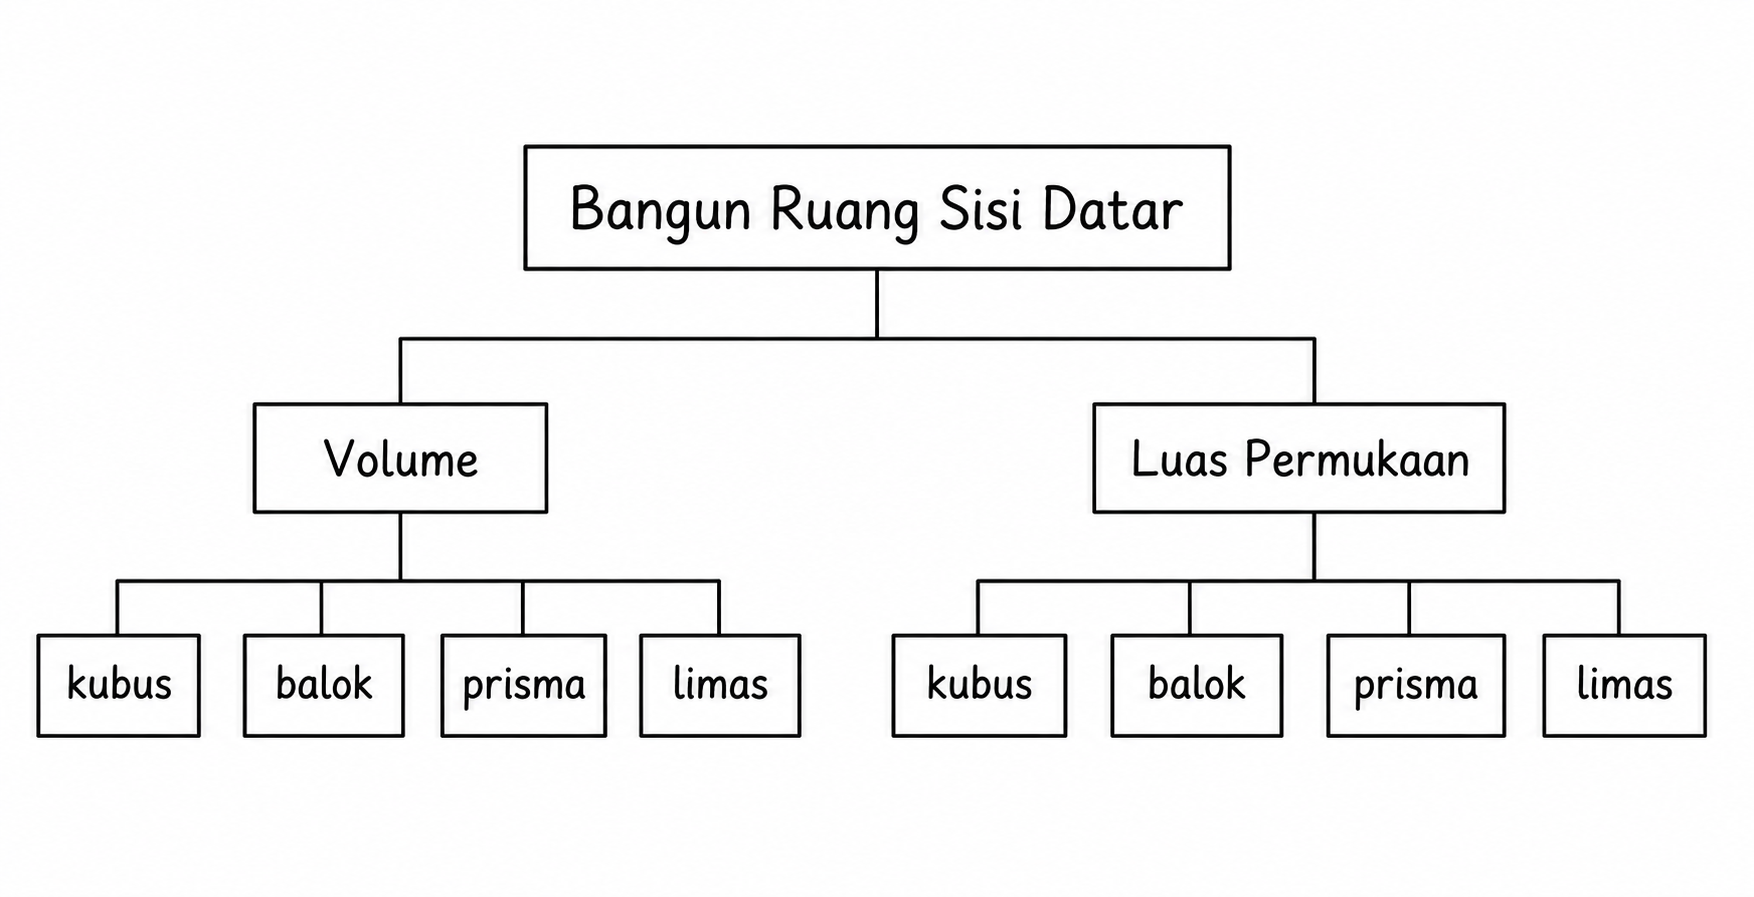
\includegraphics[width=0.8\textwidth]{images/bagan2.png}
            \caption{Struktur Hirarki Materi Bangun Ruang Sisi Datar}
            \label{fig:strukturmateri}
        \end{figure}
        Dari materi yang telah ditentukan, peneliti memilih beberapa materi yang dapat dijelaskan dengan simulasi 3D, yaitu:
        \begin{enumerate}[label=\arabic*.]
            \item Simulasi konsep volume pada kubus, menghitung banyaknya kubus satuan yang menyusun sebuah kubus.
            \item Simulasi konsep volume pada limas, sebuah kubus yang dapat berubah menjadi tiga buah limas dengan ukuran yang sama.
            \item Simulasi jaring-jaring bangun ruang kubus, balok, prisma, dan limas.
        \end{enumerate}
        \item Perancangan Media \\
        \hspace*{1cm}Terlebih dahulu peneliti merancang tampilan media dalam bentuk \textit{wireframe}. \textit{Wireframe} ini berfungsi sebagai panduan dalam membuat tampilan antarmuka pengguna (UI) media pembelajaran yang akan dikembangkan.
        \begin{figure}[H]
            \centering
            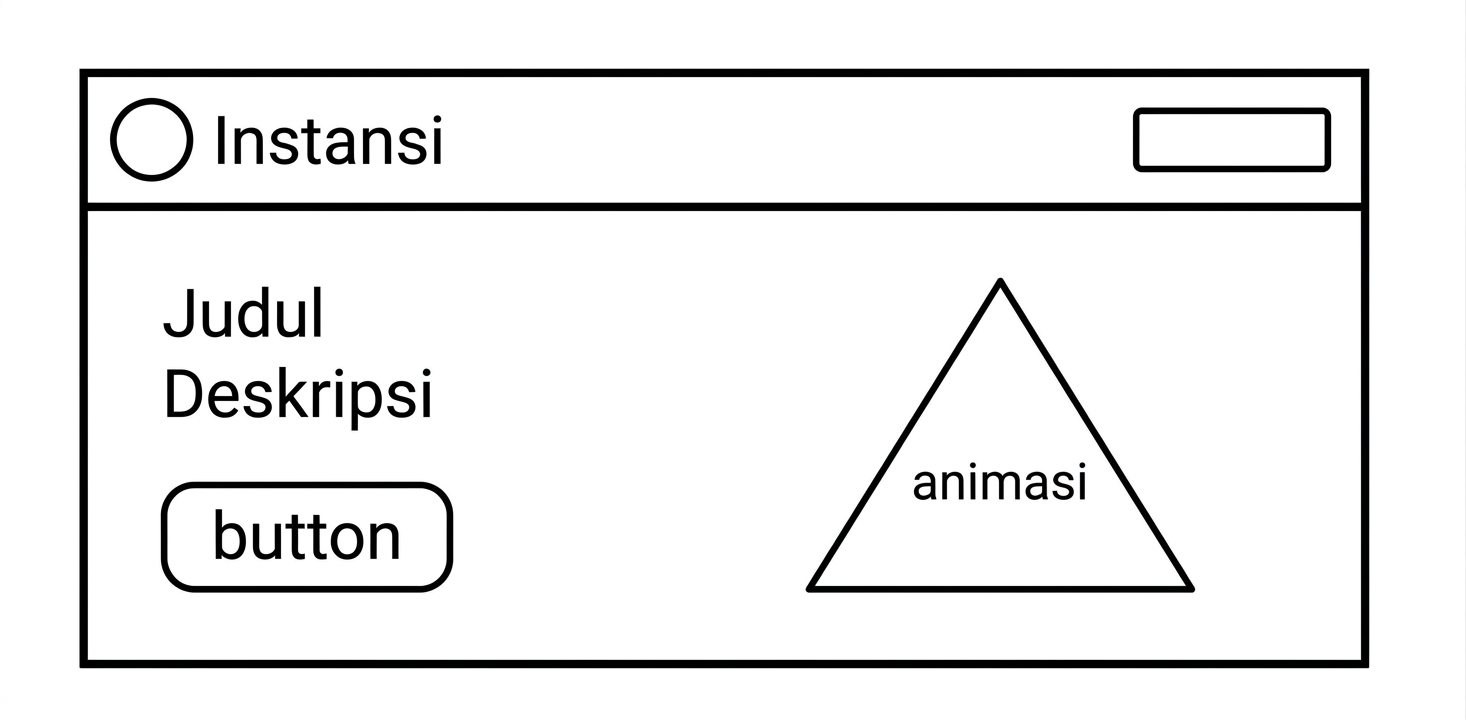
\includegraphics[width=0.8\textwidth]{images/landingpage2.png}
            \caption{Landing Page}
            \label{fig:landingpage}
        \end{figure}
        \begin{figure}[H]
            \centering
            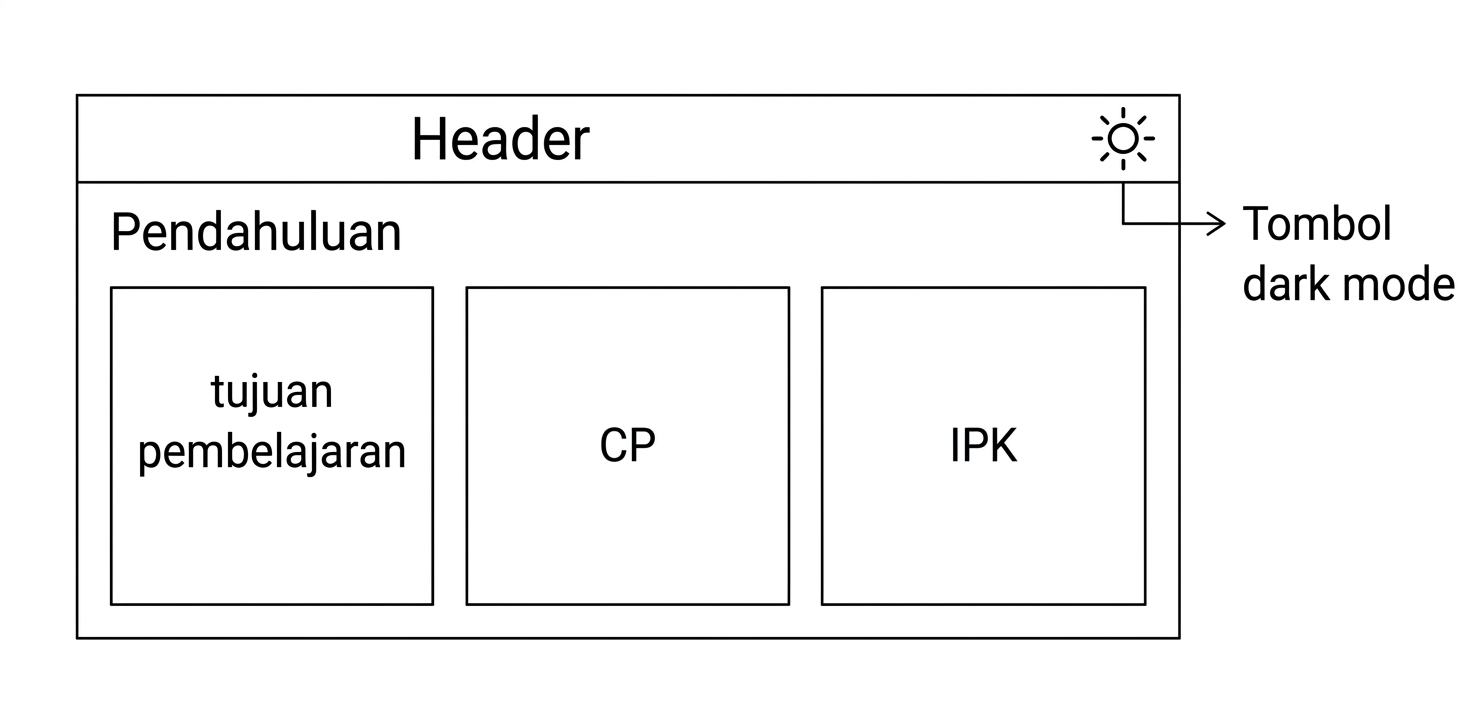
\includegraphics[width=0.8\textwidth]{images/pendahuluan2.png}
            \caption{Halaman Pendahuluan}
            \label{fig:pendahuluan}
        \end{figure}
        \begin{figure}[H]
            \centering
            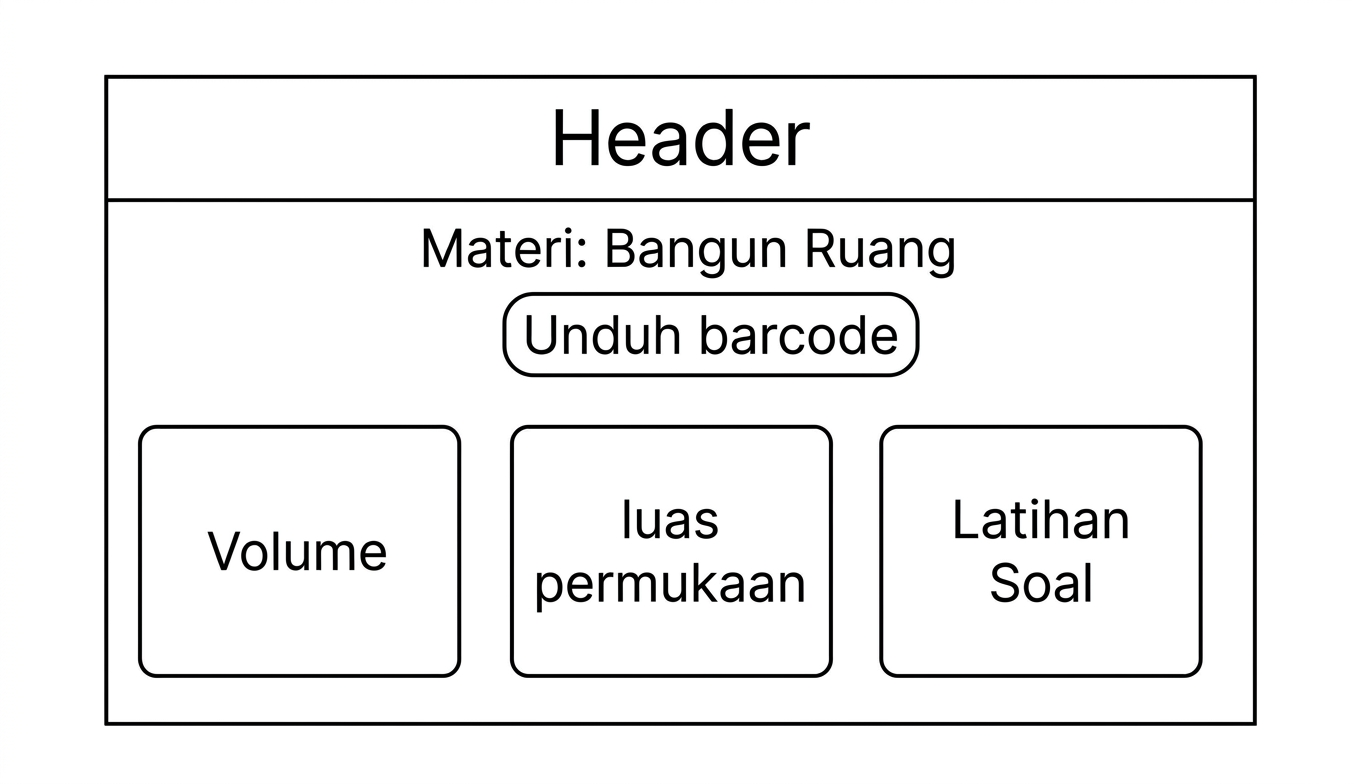
\includegraphics[width=0.8\textwidth]{images/menu2.png}
            \caption{Halaman Menu}
            \label{fig:halamanmenu}
        \end{figure}
        \begin{figure}[H]
            \centering
            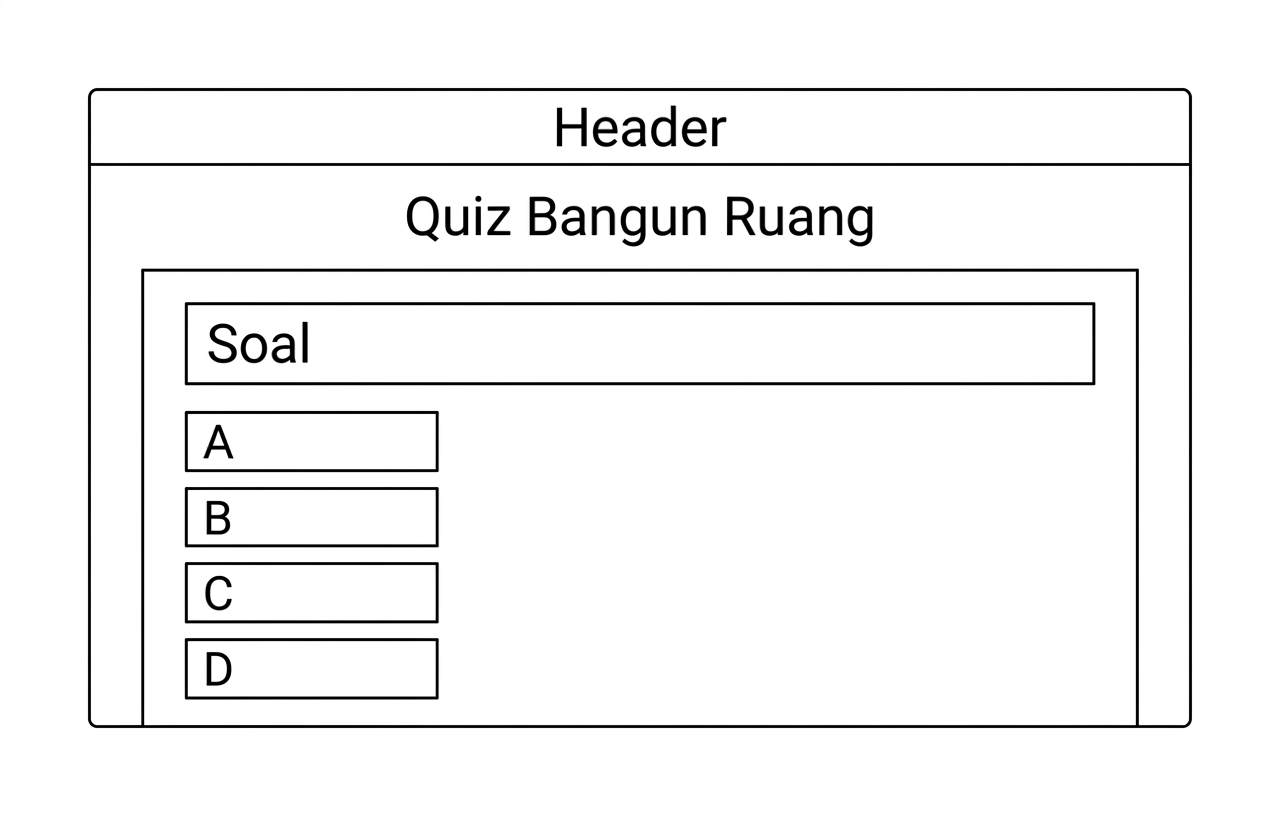
\includegraphics[width=0.8\textwidth]{images/quiz2.png}
            \caption{Halaman Quiz}
            \label{fig:halamanquiz}
        \end{figure}
        Selain merancang tampilan antarmuka pengguna (UI) melalui \textit{wireframe}, peneliti juga membuat diagram alur navigasi website untuk mengilustrasikan struktur dan aliran interaksi pengguna dalam sistem. Diagram alur navigasi ini dirancang untuk memastikan kemudahan navigasi dan pengalaman pengguna yang optimal. Berikut adalah rancangan alur navigasi yang telah dibuat:
        \begin{figure}[H]
            \centering
            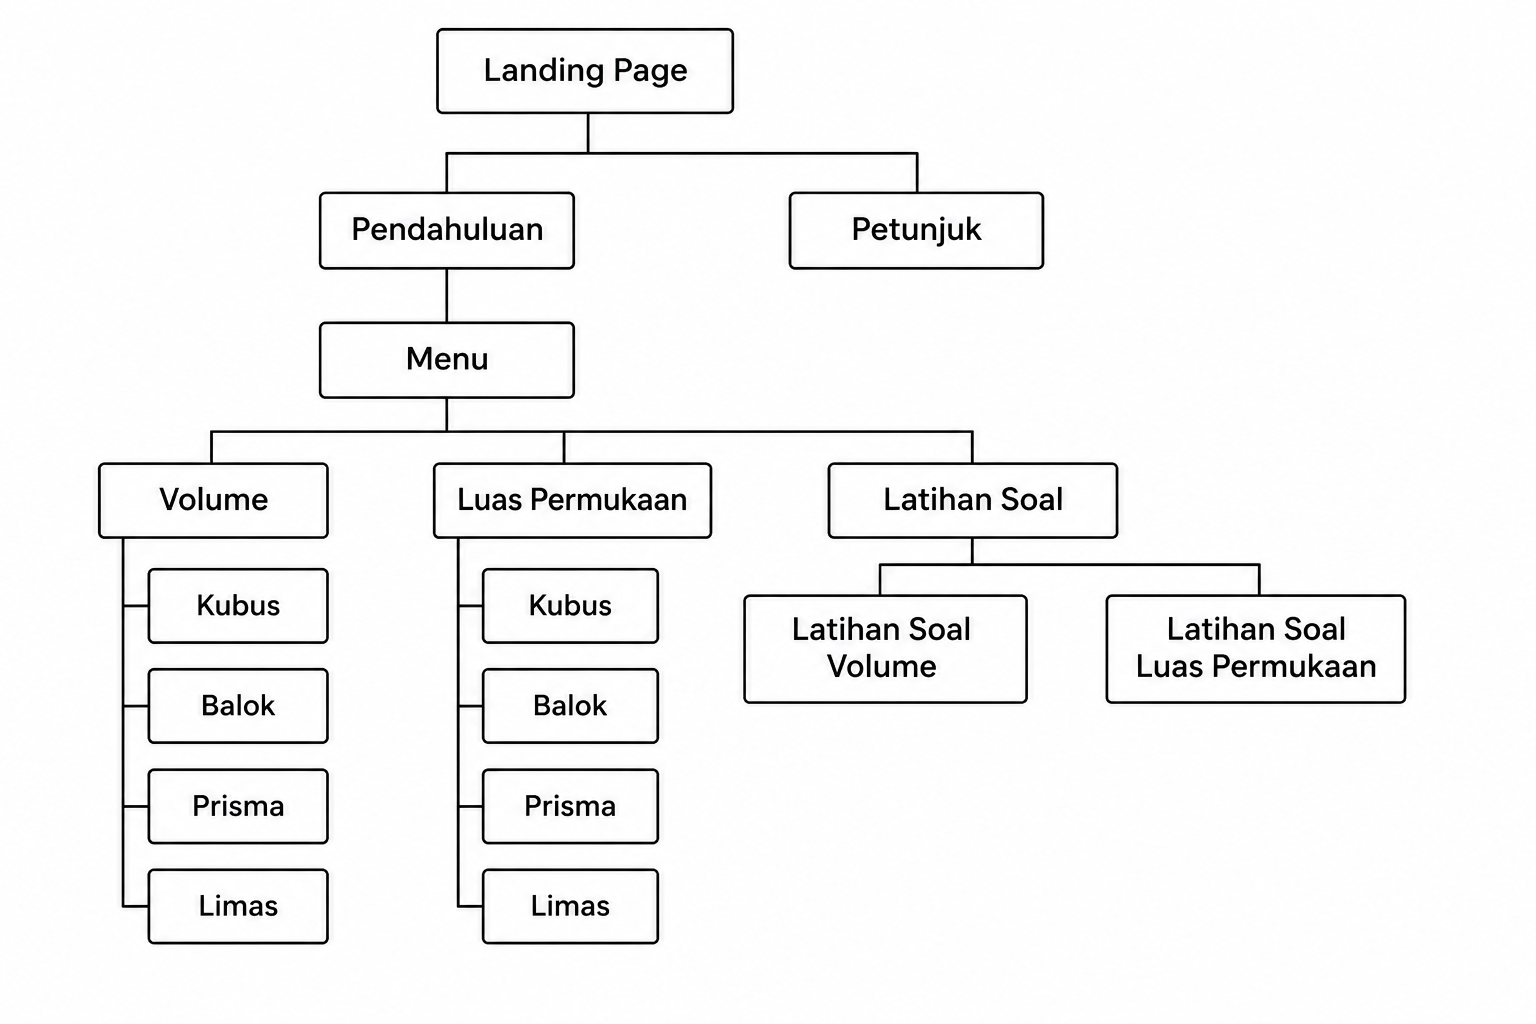
\includegraphics[width=0.8\textwidth]{images/Flow.png}
            \caption{Diagram Alur Navigasi Website}
            \label{fig:flowchart}
        \end{figure}
        \item Perancangan Interaksi Simulasi 3D
        \begin{figure}[H]
            \centering
            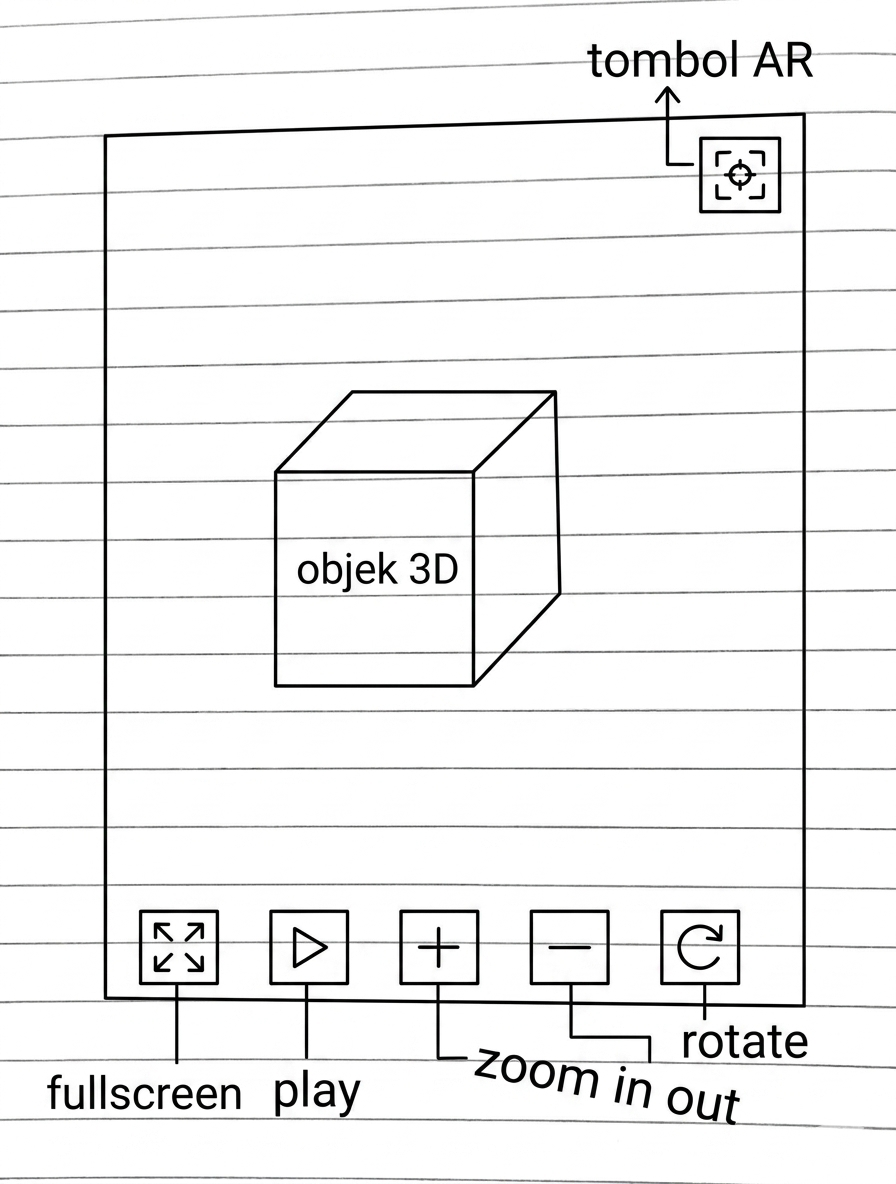
\includegraphics[width=0.5\textwidth]{images/mocksimulasi3d.png}
            \caption{Halaman Simulasi 3D}
            \label{fig:mocksimulasi3d}
        \end{figure}
        \hspace*{1cm}Desain antarmuka halaman simulasi 3D ditampilkan pada Gambar \ref{fig:mocksimulasi3d}. Pada tampilan tersebut terdapat model 3D di tengah layar yang dapat dikendalikan melalui beberapa kontrol utama, antara lain:
        \begin{table}[H]
            \centering
            \caption{Kontrol Utama Pada Halaman Simulasi 3D}
            \label{tab:kontrolsimulasi3d}
            \begin{tabular}{|p{3.5cm}|p{9cm}|}
                \hline
                \textbf{Kontrol} & \textbf{Fungsi} \\
                \hline
                Fullscreen & Berpindah ke tampilan layar penuh untuk memperbesar area visualisasi. \\
                \hline
                Play / Pause & Menjalankan atau menghentikan animasi model 3D. \\
                \hline
                Zoom In / Zoom Out & Memperbesar atau memperkecil tampilan objek untuk melihat detail atau konteks keseluruhan. \\
                \hline
                Rotate & Memutar objek dengan kecepatan konstan; fitur ini dapat diaktifkan atau dinonaktifkan oleh pengguna. \\
                \hline
                AR & Berpindah ke mode \textit{Augmented Reality (AR)} menggunakan model 3D yang sama. \\
                \hline
            \end{tabular}
        \end{table}
        \item Perancangan Model 3D\\
        \hspace*{1cm}Model 3D dibuat menggunakan perangkat lunak Blender. Model yang dibuat meliputi kubus, balok, prisma, limas, serta jaring-jaring masing-masing bangun ruang. Semua model diekspor dalam format \texttt{.glb}.
        \item Perancangan Arsitektur Website\\
        \hspace*{1cm}Arsitektur website dirancang sebagai aplikasi frontend berbasis \textbf{React} yang berperan sebagai \textit{Single Page Application (SPA)}. Pengembangan dilakukan secara lokal oleh tim pengembang menggunakan \textbf{Node.js} dan pengelola paket  \textbf{yarn}; seluruh kode sumber dikelola pada repositori GitHub. Struktur penyimpanan dan alur data dirancang sebagai berikut:

        \begin{enumerate}[leftmargin=*, label=--]
            \item Asset statis (gambar, berkas grafis) dan model 3D (format \texttt{.glb}) disimpan pada layanan Supabase Storage dan disajikan melalui URL publik untuk akses cepat oleh klien.
            \item Komponen simulasi 3D diimplementasikan di sisi klien menggunakan \textbf{Three.js} di dalam komponen React, sehingga rendering dan interaksi (zoom, rotate, animasi) dijalankan di browser pengguna.
            \item Integrasi AR dilakukan melalui layanan eksternal \textbf{mywebar.com}, di mana model 3D yang sama diunggah dan dikonfigurasi untuk mode AR. Link atau QR code yang dihasilkan oleh mywebar.com diintegrasikan ke dalam aplikasi React untuk akses langsung ke fitur AR.
            \item Variabel lingkungan sensitif (kunci API, URL storage) disimpan sebagai secret pada pengaturan Vercel dan tidak dikomit ke repositori.
            \item \textit{Continuous Deployment (CD)}: setiap perubahan yang dipush ke cabang utama pada GitHub memicu proses build otomatis di Vercel, yang meliputi instalasi dependensi, proses bundling React, dan penerapan ke domain produksi \textbf{https://medpemar.vercel.app}.
        \end{enumerate}

        \hspace*{1cm}Peneliti merancang arsitektur website dengan mempertimbangkan pemisahan tugas, kemudahan pemeliharaan, dan skalabilitas. Arsitektur ini memungkinkan pengembangan fitur tambahan di masa depan, seperti penambahan materi pembelajaran baru atau peningkatan interaktivitas simulasi 3D, tanpa perlu merombak keseluruhan sistem. Desain arsitektur website dapat dilihat pada Gambar \ref{fig:arsitekturweb} berikut.
        \begin{figure}[H]
            \centering
            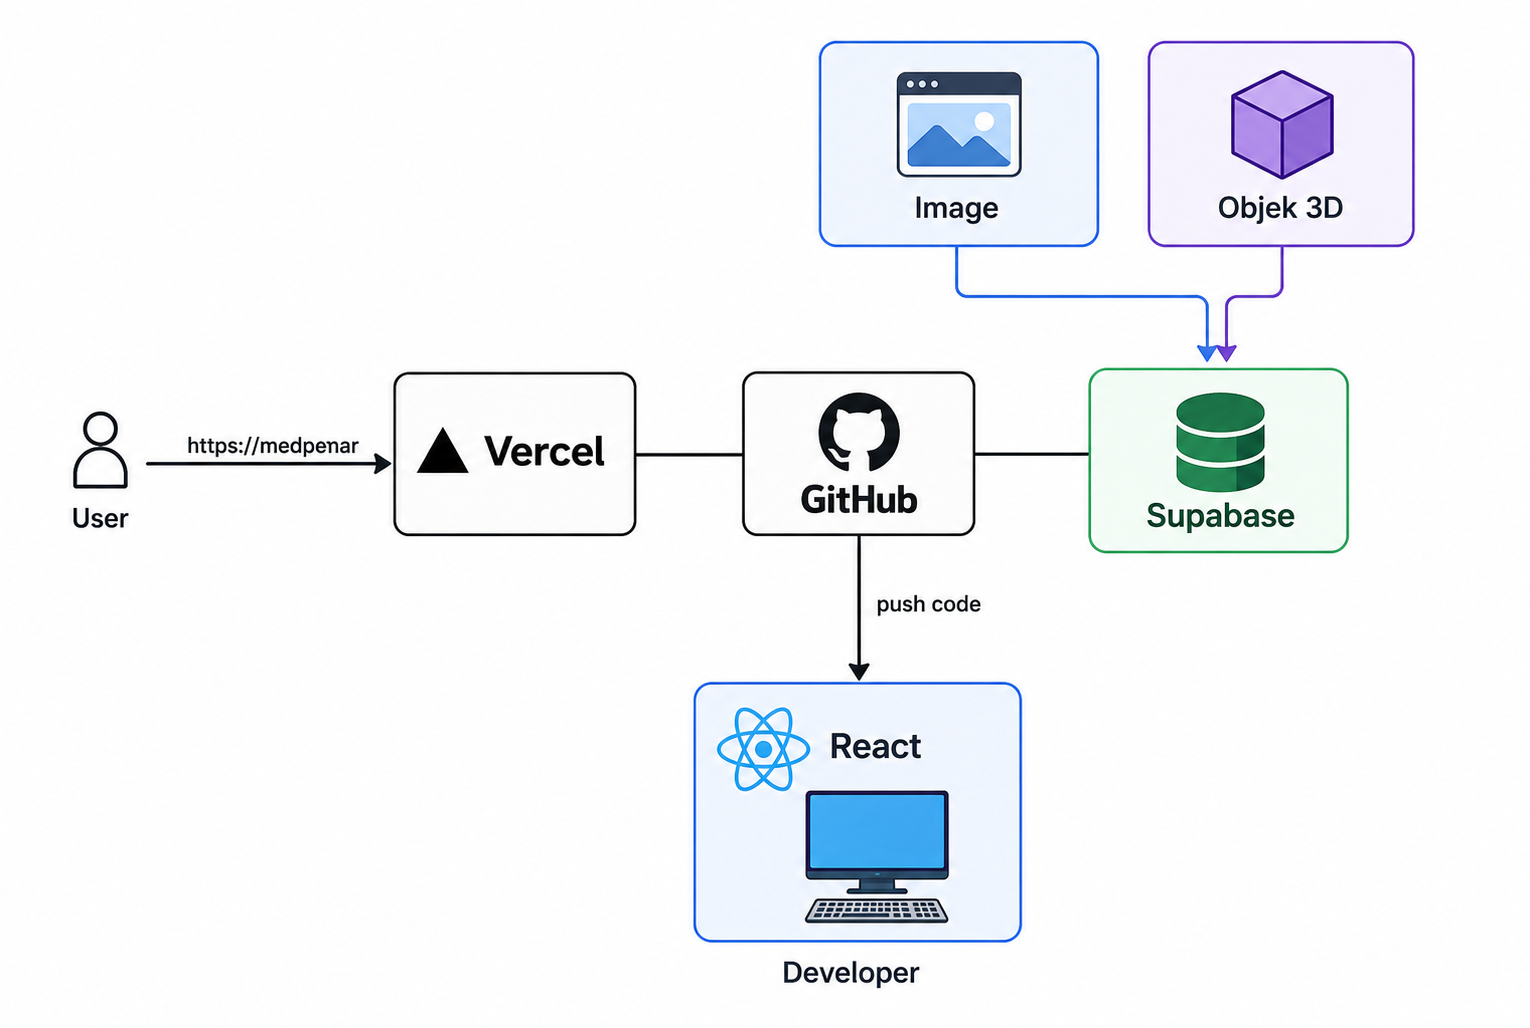
\includegraphics[width=0.9\textwidth]{images/Arsitektur.png}
            \caption{Arsitektur Website}
            \label{fig:arsitekturweb}
        \end{figure}

        

    \end{enumerate}

    \item \textbf{Pengembangan \textit{(Development)}}\\
    \hspace*{1cm}Pengembangan media pembelajaran berbasis simulasi 3D tergolong kompleks. Pengembangan simulasi 3D menggunakan React dan Blender sendiri merupakan hal baru dalam dunia pendidikan, sehingga referensi untuk pengembangannya masih terbatas. Tahapan yang dilakukan peneliti meliputi implementasi desain, pengembangan antarmuka, pengembangan fitur simulasi 3D, pembuatan model 3D, pengembangan fitur evaluasi, integrasi sistem, validasi produk, dan revisi produk. Berikut adalah penjabaran dari masing-masing tahapan tersebut.
    
    \begin{enumerate}[label=\arabic*)]
        \item Implementasi Desain\\
        \hspace*{1cm}Sesuai dengan arsitektur website pada Gambar \ref{fig:arsitekturweb}, proses implementasi mencakup beberapa langkah teknis utama. Tahap ini dimulai dengan konfigurasi layanan penyimpanan file pada Supabase dan pembuatan repositori kode di GitHub. Selanjutnya, kode sumber di-*clone* ke lingkungan pengembangan lokal, kemudian dilakukan instalasi dependensi, termasuk React dan library pendukung lainnya, sebelum memulai pengembangan antarmuka.
        \begin{enumerate}[leftmargin=*, label=--]
            \item Mengonfigurasi penyimpanan di Supabase untuk menyimpan gambar, model 3D, dan aset pendukung.
            \item Menyiapkan repositori di GitHub sebagai basis kode sumber dan pengelolaan versi.
            \item Meng-clone repositori ke lingkungan pengembangan lokal.
            \item Menginstal dependensi yang diperlukan untuk proyek React, termasuk paket untuk Three.js.
            \item Memulai pengembangan antarmuka pengguna berdasarkan desain yang telah ditetapkan.
        \end{enumerate}
        \begin{figure}[H]
            \centering
            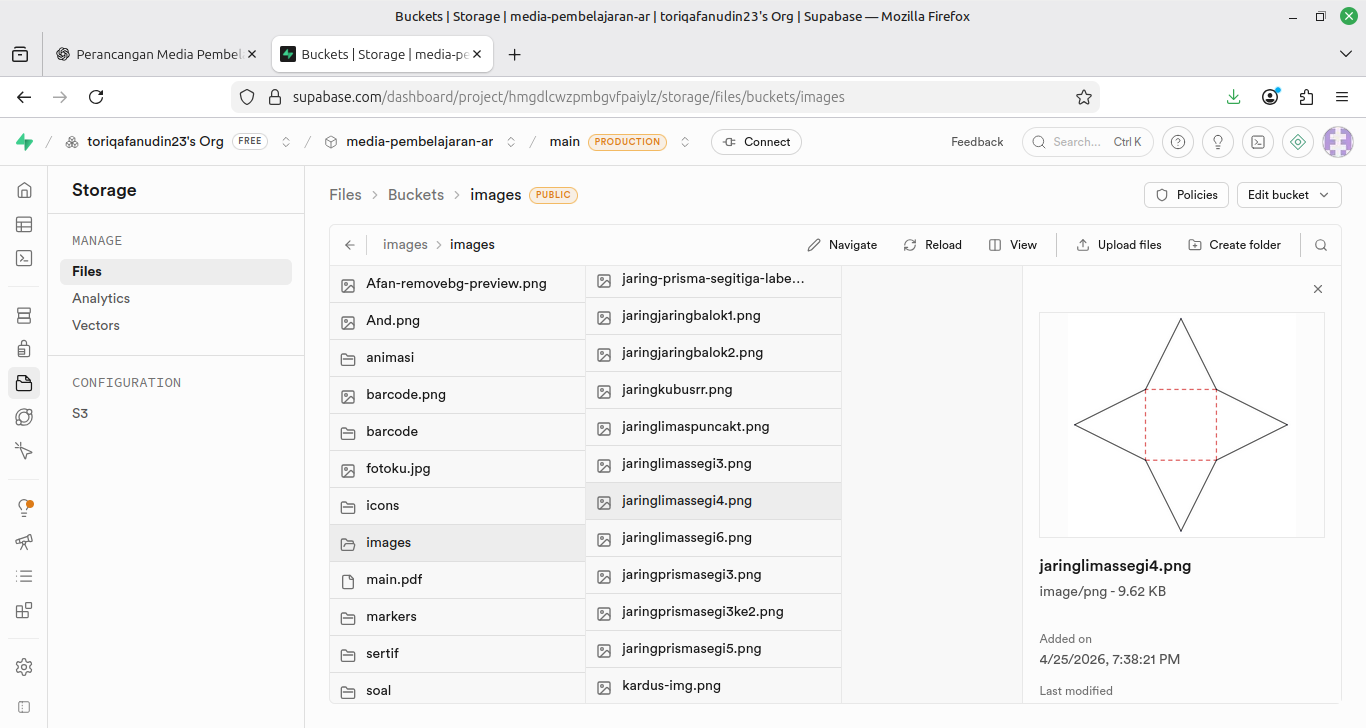
\includegraphics[width=1\textwidth]{images2/supabase.png}
            \caption{Storage di Supabase}
            \label{fig:supabase}
        \end{figure}
        \begin{figure}[H]
            \centering
            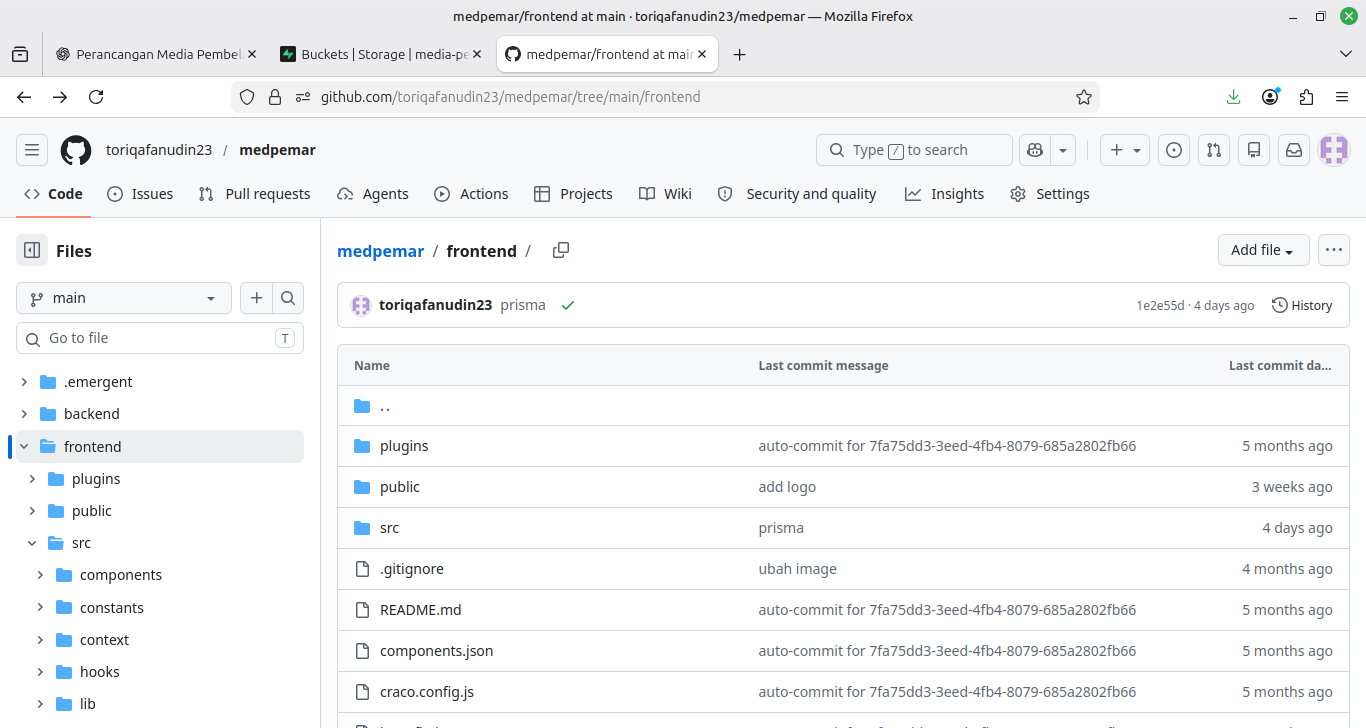
\includegraphics[width=1\textwidth]{images2/github.png}
            \caption{Repository di Github}
            \label{fig:github}
        \end{figure}
        \item Pengembangan Antarmuka\\
        \hspace*{1cm}Pengembangan antarmuka dilakukan menggunakan \textbf{React} sebagai library utama untuk membangun \textit{Single Page Application (SPA)}. Antarmuka aplikasi dirancang responsif untuk berbagai ukuran layar dan perangkat. Peneliti mengintegrasikan \textbf{Three.js} untuk menampilkan dan memanipulasi model 3D langsung di dalam halaman website. Komponen React dikembangkan untuk mengelola status aplikasi, navigasi halaman, dan komunikasi dengan API eksternal. Berikut ditampilkan contoh hasil pengembangan antarmuka.
        \begin{figure}[H]
            \centering
            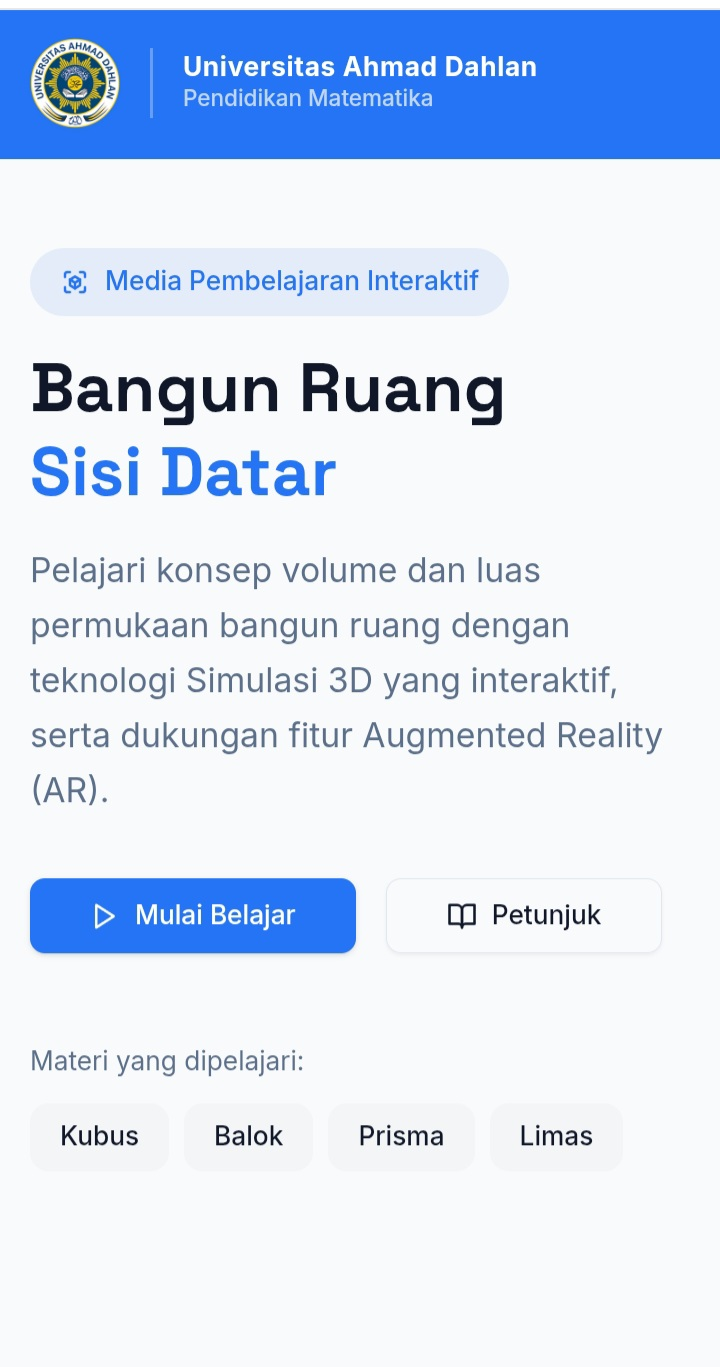
\includegraphics[width=0.3\textwidth]{images2/landingpage.jpg}
            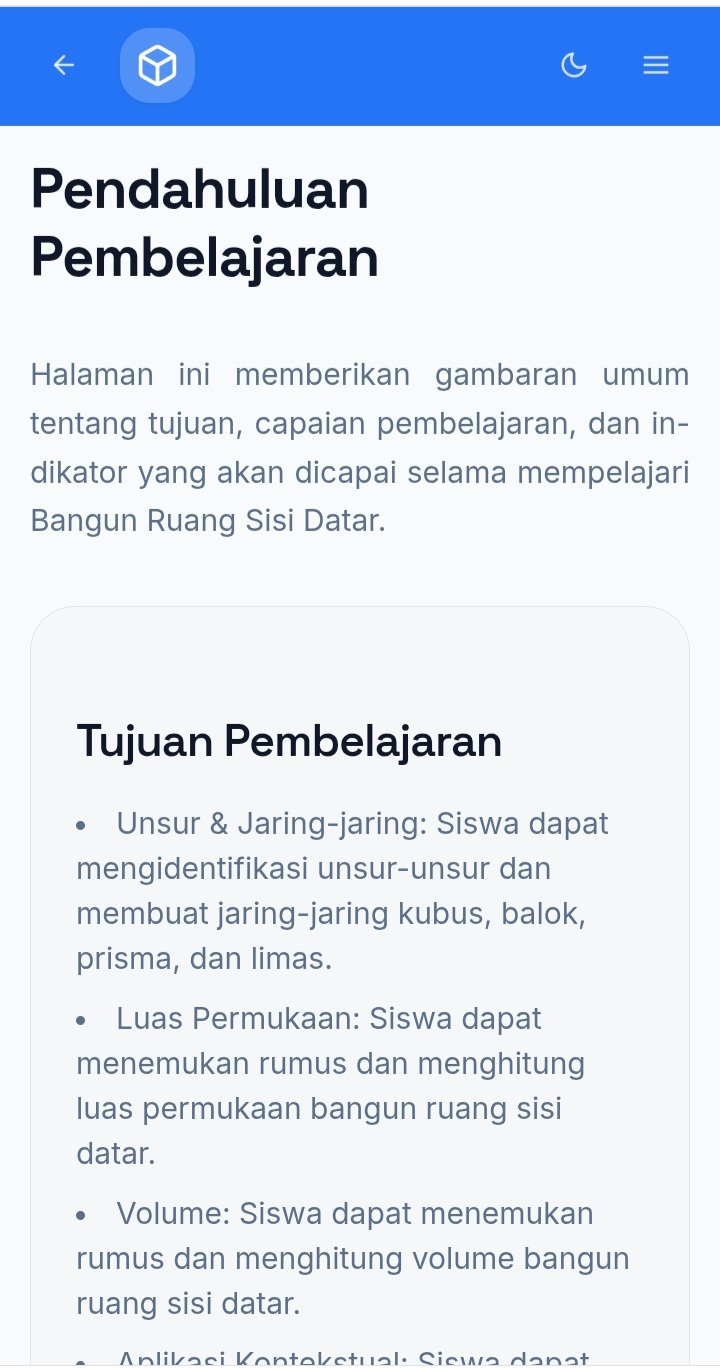
\includegraphics[width=0.3\textwidth]{images2/tujuanpembelajaran.jpg}
            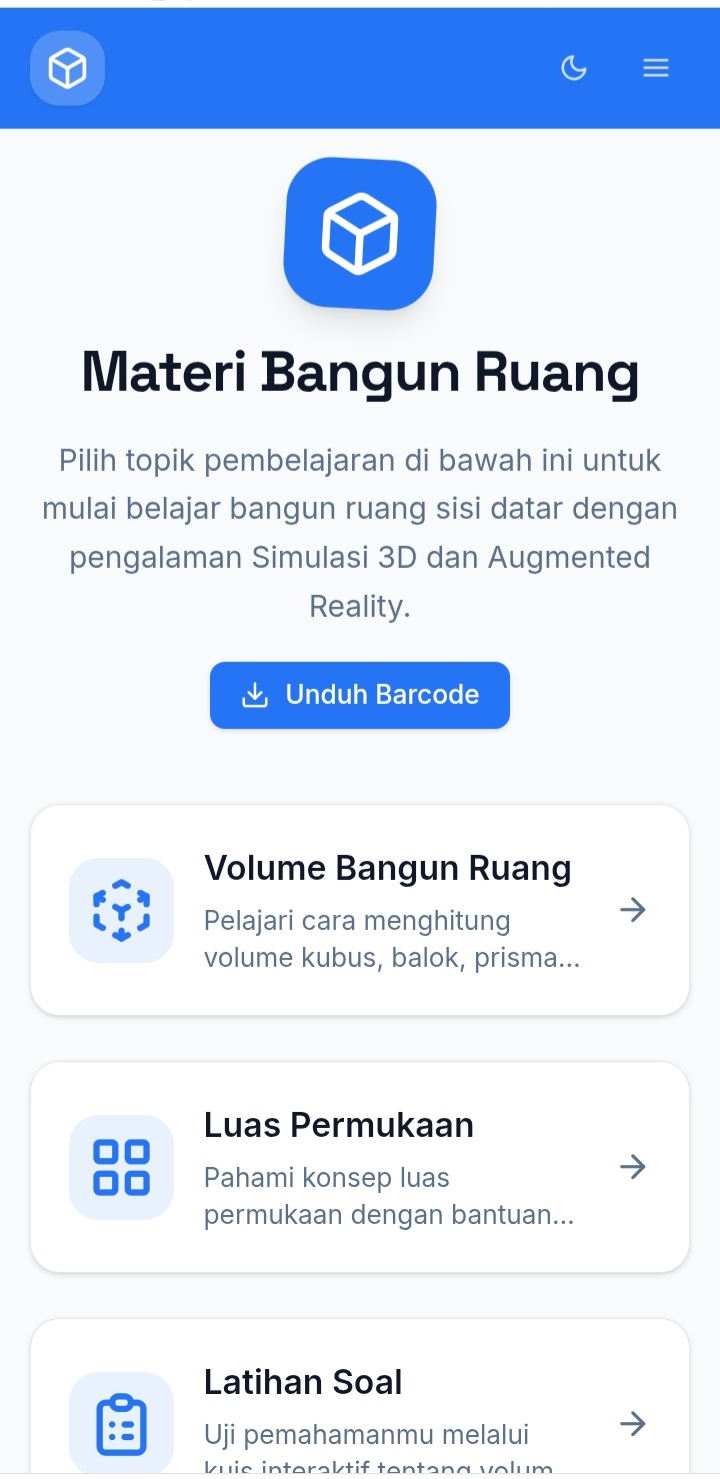
\includegraphics[width=0.3\textwidth]{images2/menu.jpg}
            \caption{Contoh Antarmuka Media Pembelajaran}
            \label{fig:antarmuka}
        \end{figure}

        \item Pembuatan Model 3D\\
        \hspace*{1cm}Pembuatan model 3D dilakukan menggunakan aplikasi \textbf{Blender}, yang merupakan perangkat lunak gratis dan open-source untuk pemodelan 3D dan animasi. Peneliti membuat model berbentuk kubus, balok, prisma, dan limas dengan detail geometri yang akurat sesuai dengan materi bangun ruang sisi datar. Selain itu, dikembangkan juga animasi jaring-jaring yang dapat menunjukkan proses pembukaan bangun ruang menjadi jaring-jaringnya, untuk meningkatkan pemahaman peserta didik. Semua model 3D diekspor ke format \texttt{.glb} (glTF binary format) untuk kompatibilitas maksimal dengan Three.js. Berikut tampilan aplikasi Blender dan contoh model 3D yang dihasilkan.
        \begin{figure}[H]
            \centering
            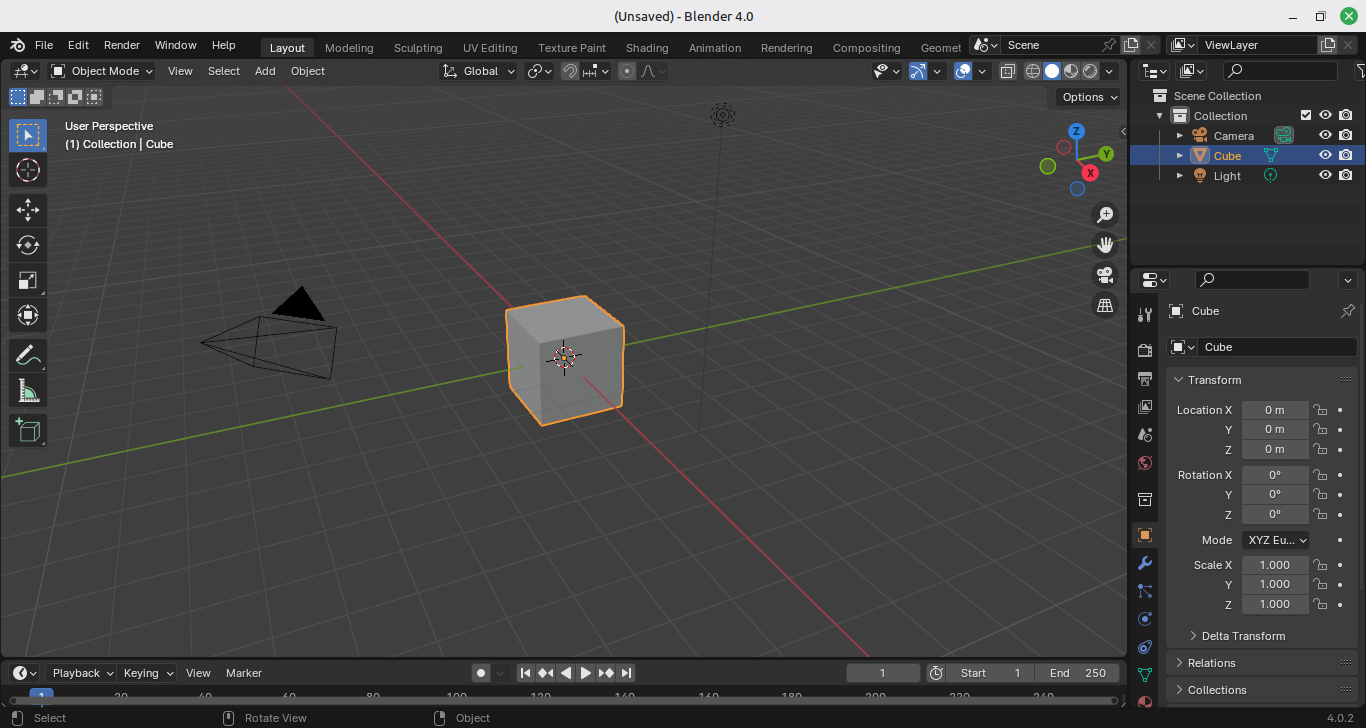
\includegraphics[width=1\textwidth]{images2/blender.png}
            \caption{Pembuatan Model 3D dengan Blender}
            \label{fig:blender}
        \end{figure}
        \begin{figure}[H]
            \centering
            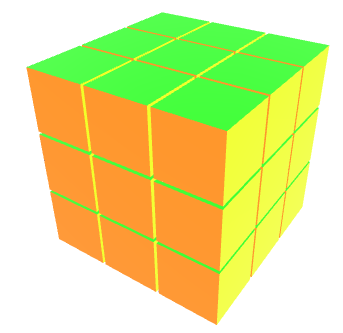
\includegraphics[width=0.3\textwidth]{images2/kubus.png}
            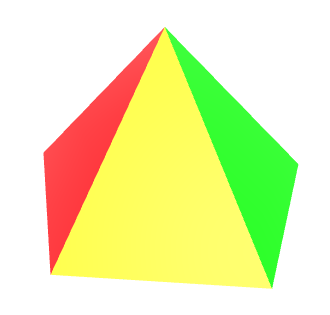
\includegraphics[width=0.3\textwidth]{images2/limas.png}
            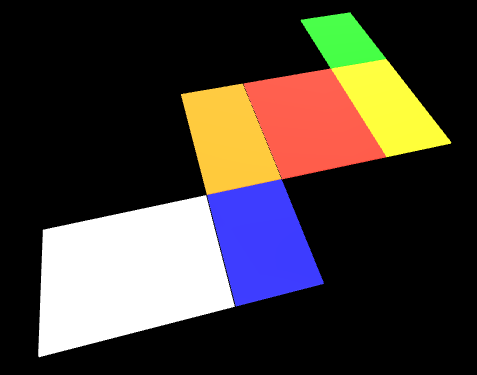
\includegraphics[width=0.3\textwidth]{images2/jaringbalok.png}
            \caption{Contoh Model 3D}
            \label{fig:contohobjek3d}
        \end{figure}
        
        \item Pengembangan Fitur Simulasi 3D\\
        \hspace*{1cm}Pengembangan simulasi 3D dilakukan berdasarkan desain yang ditampilkan pada Gambar 15. Simulasi 3D diimplementasikan menggunakan library \textbf{Three.js} dalam komponen React untuk menampilkan dan memanipulasi model bangun ruang secara interaktif. Model 3D yang telah dibuat diupload ke dalam penyimpanan Supabase, kemudian komponen React yang dibuat dengan Three.js mengakses model 3D tersebut untuk ditampilkan di dalam website.
        
        \hspace*{1cm}Fitur simulasi 3D memiliki beberapa tombol utama untuk mengontrol model 3D secara interaktif. Adapun daftar tombol yang tersedia bisa dilihat pada Tabel \ref{tab:kontrolsimulasi3d}. Melalui simulasi 3D interaktif ini, peserta didik dapat memahami konsep-konsep matematika abstrak antara lain:
        \begin{enumerate}[leftmargin=*, label=--]
            \item \textbf{Volume kubus:} Visualisasi kubus besar yang tersusun dari kubus-kubus satuan, membantu peserta didik memahami konsep volume sebagai pengisian ruang tiga dimensi.
            \item \textbf{Volume limas:} Animasi yang menunjukkan transformasi kubus menjadi tiga limas dengan ukuran yang sama, memperjelas hubungan antara volume kubus dan limas.
            \item \textbf{Jaring-jaring:} Animasi pembukaan berbagai bangun ruang (kubus, balok, prisma, limas) menjadi jaring-jaringnya, memfasilitasi pemahaman hubungan antara bentuk 3D dan representasi 2D.
        \end{enumerate}
        
        \hspace*{1cm}Desain lengkap simulasi 3D dengan tampilan antarmuka, tombol kontrol, dan visualisasi objek dapat dilihat pada Gambar \ref{fig:simulasi3d} berikut:
        \begin{figure}[H]
            \centering
            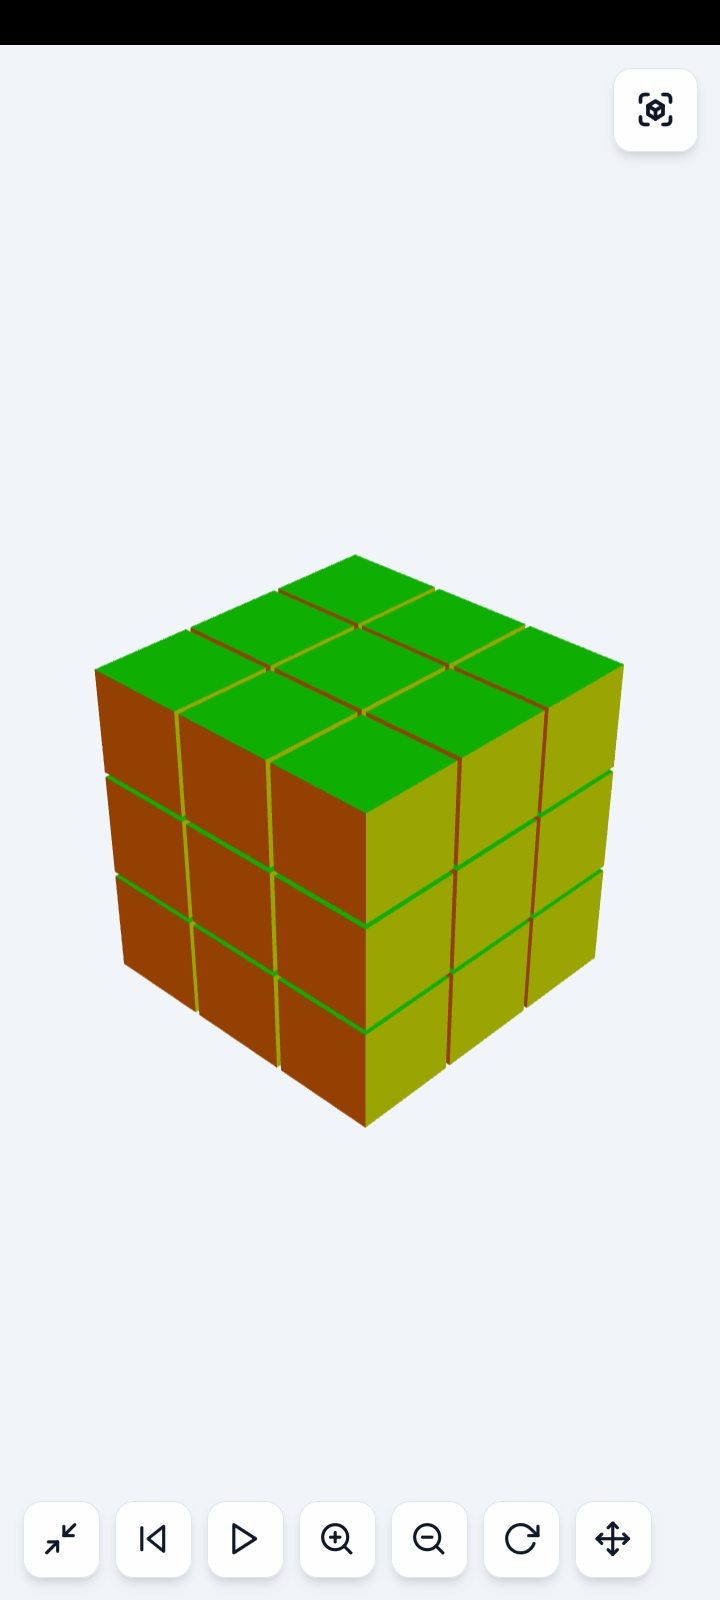
\includegraphics[width=0.35\textwidth]{images2/simulasi3d.jpg}
            \caption{Tampilan Simulasi 3D}
            \label{fig:simulasi3d}
        \end{figure}
        
        
        \item Menampilkan Model 3D melalui Fitur \textit{Augmented Reality (AR)}\\
        \hspace*{1cm}Untuk memperkaya pengalaman pembelajaran, peneliti mengintegrasikan fitur \textit{Augmented Reality (AR)} yang memungkinkan peserta didik melihat model 3D bangun ruang dalam lingkungan nyata mereka. Implementasi AR dilakukan menggunakan layanan online \textbf{MyWebAR}, yang merupakan \textit{platform user-friendly} untuk mengubah model 3D menjadi konten AR tanpa memerlukan pemrograman yang rumit.
        
        \hspace*{1cm}Keunggulan menggunakan layanan mywebar.com antara lain:
        \begin{enumerate}[leftmargin=*, label=--]
            \item Interface yang intuitif dan mudah digunakan bahkan bagi pengguna awam.
            \item Animasi dari model 3D tetap berfungsi setelah dikonversi menjadi konten AR, sehingga fitur interaktif seperti rotasi dan transformasi jaring-jaring masih dapat diakses dalam mode AR.
            \item Sifat layanan yang berbasis cloud (online) memungkinkan integrasi mudah dengan aplikasi website yang sedang dikembangkan.
        \end{enumerate}
        
        \hspace*{1cm}Proses pengembangan fitur AR mencakup: (1) mengupload model 3D dalam format \texttt{.glb} ke mywebar.com, (2) melakukan konfigurasi dan kustomisasi tampilan AR, (3) menghasilkan link atau QR code yang dapat dipanggil dari aplikasi React, dan (4) mengintegrasikan link AR tersebut ke dalam komponen website sehingga peserta didik dapat mengakses fitur AR langsung dari media pembelajaran. Integrasi ini memfasilitasi pembelajaran multimodal di mana peserta didik dapat beralih antara visualisasi simulasi 3D dalam aplikasi website dan visualisasi AR di lingkungan fisik mereka.
        \begin{figure}[H]
            \centering
            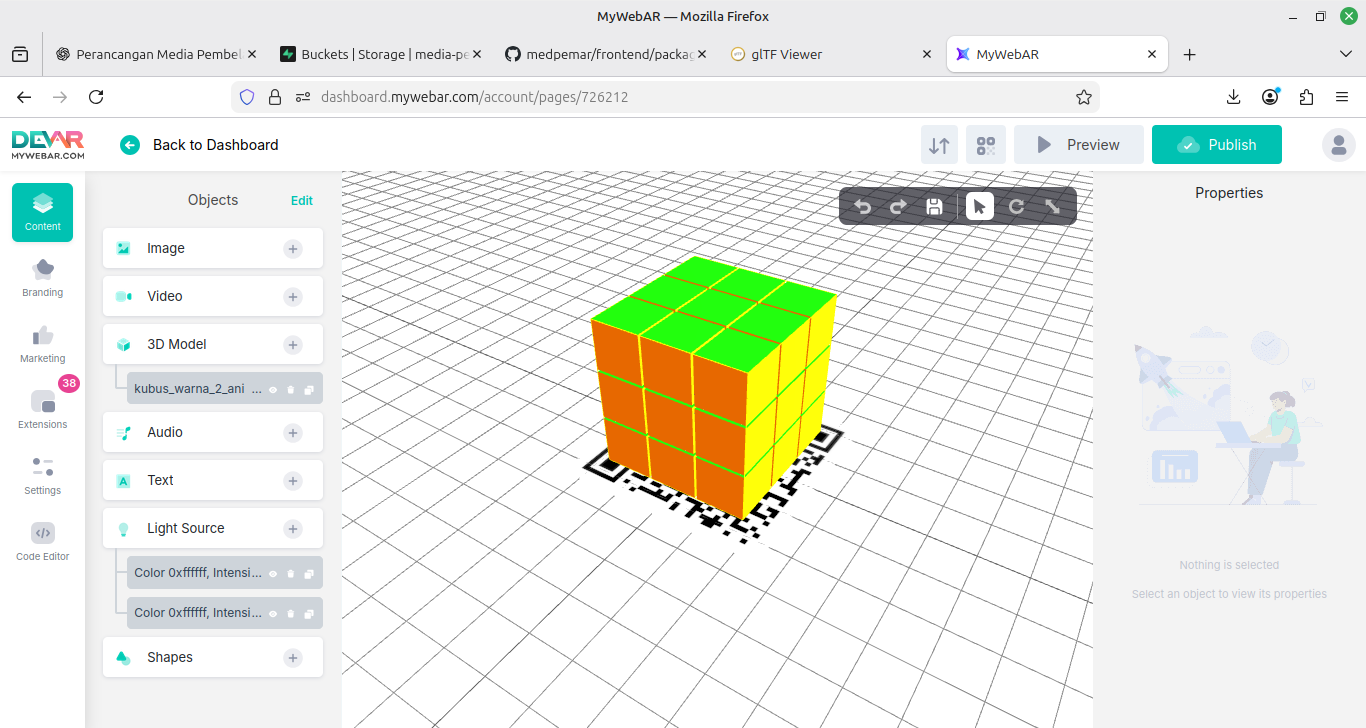
\includegraphics[width=1\textwidth]{images2/mywebar.png}
            \caption{Tampilan mywebar.com untuk Pengembangan AR}
            \label{fig:mywebar}
        \end{figure}
        \begin{figure}[H]
            \centering
            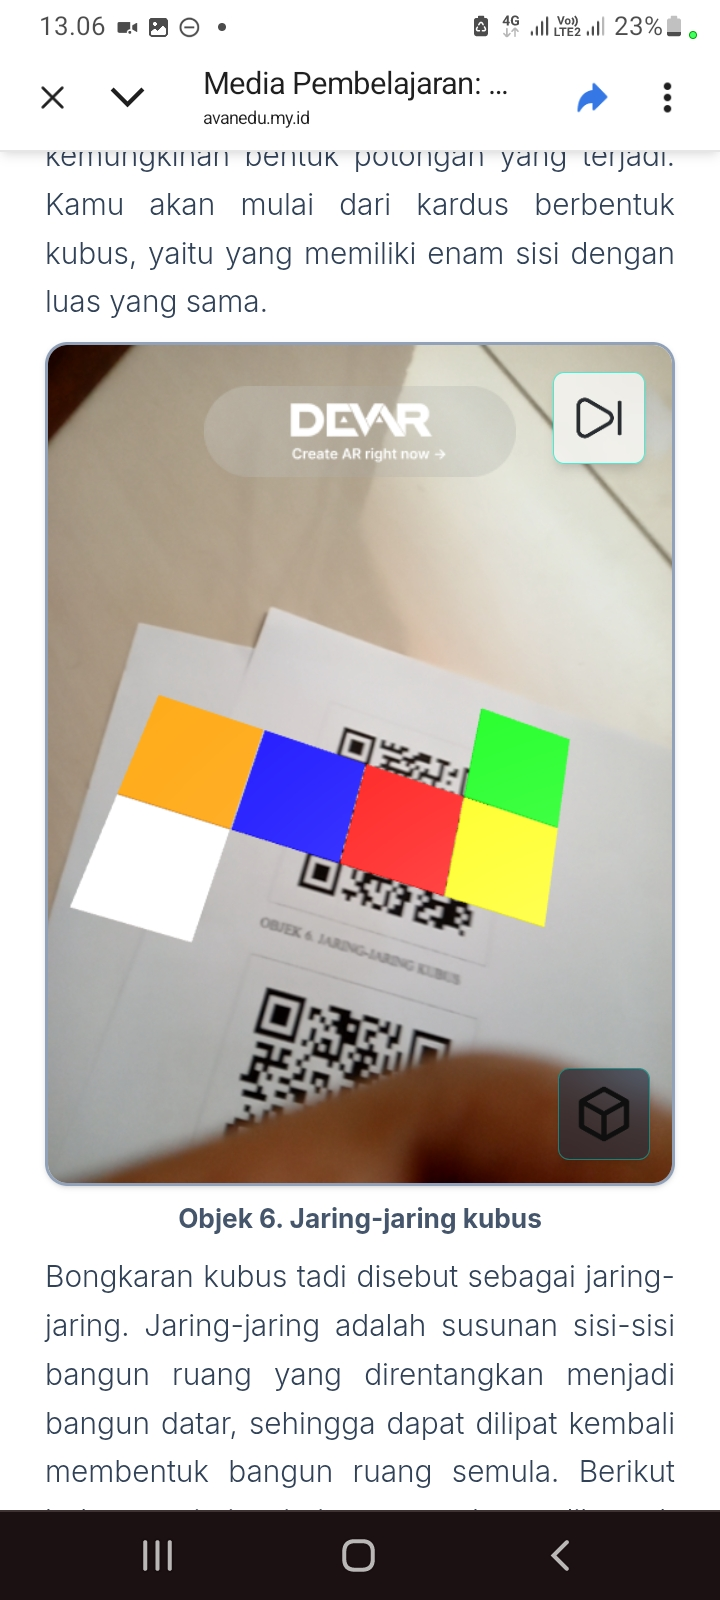
\includegraphics[width=0.3\textwidth]{images/materi4.jpg}
            \caption{Tampilan AR pada Media Pembelajaran}
            \label{fig:armedia}
        \end{figure}
        
        \item Pengembangan Evaluasi\\
        \hspace*{1cm}Pengembangan evaluasi mencakup integrasi berbagai mekanisme penilaian formatif dan sumatif dalam aplikasi untuk mendukung proses pembelajaran peserta didik. Sistem evaluasi dirancang untuk memberikan umpan balik instan dan mendukung pembelajaran mandiri. Berikut adalah komponen-komponen evaluasi yang dikembangkan:
        
        \begin{enumerate}[leftmargin=*, label=--]
            \item \textbf{Isian Singkat dalam Proses Pembelajaran:} Selama pembelajaran, peneliti menyisipkan pertanyaan isian singkat pada tahap-tahap strategis untuk memastikan peserta didik memahami konsep sebelum melanjutkan ke materi selanjutnya. Jika jawaban peserta didik benar, sistem memberikan umpan balik positif. Mekanisme ini berfungsi sebagai \textit{checkpoint} pembelajaran untuk mengidentifikasi pemahaman peserta didik secara \textit{real-time}.
            
            \item \textbf{Soal Evaluasi di Akhir Setiap Bab:} Setiap bab materi diakhiri dengan serangkaian soal evaluasi komprehensif. Peserta didik dapat mengecek jawaban mereka, dan jika jawaban benar, sistem menampilkan pembahasan mendetail yang menjelaskan solusi dan konsep-konsep terkait. Fitur ini mendukung pembelajaran reflektif dan membantu peserta didik memahami alasan di balik jawaban yang benar.
            
            \item \textbf{Fitur Quiz Interaktif:} Peneliti mengembangkan dua paket kuis spesifik untuk menguji pemahaman mendalam peserta didik mengenai topik utama:
            \begin{itemize}
                \item \textbf{Quiz Volume:} Paket kuis yang fokus pada konsep volume berbagai bangun ruang sisi datar.
                \item \textbf{Quiz Luas Permukaan:} Paket kuis yang fokus pada konsep luas permukaan berbagai bangun ruang.
            \end{itemize}
            
            Setiap soal dalam kuis berbentuk pilihan ganda dengan opsi jawaban yang disusun strategis. Untuk setiap jawaban yang dipilih peserta didik, baik benar maupun salah, sistem menampilkan pembahasan detail yang menjelaskan mengapa jawaban tersebut benar atau salah dan memberikan pengajaran ulang konsep yang relevan. Setelah semua soal dalam kuis dijawab, sistem secara otomatis menghitung dan menampilkan skor akhir peserta didik, memberikan informasi tentang pencapaian mereka terhadap standar pembelajaran.
        \end{enumerate}
        \begin{figure}[H]
            \centering
            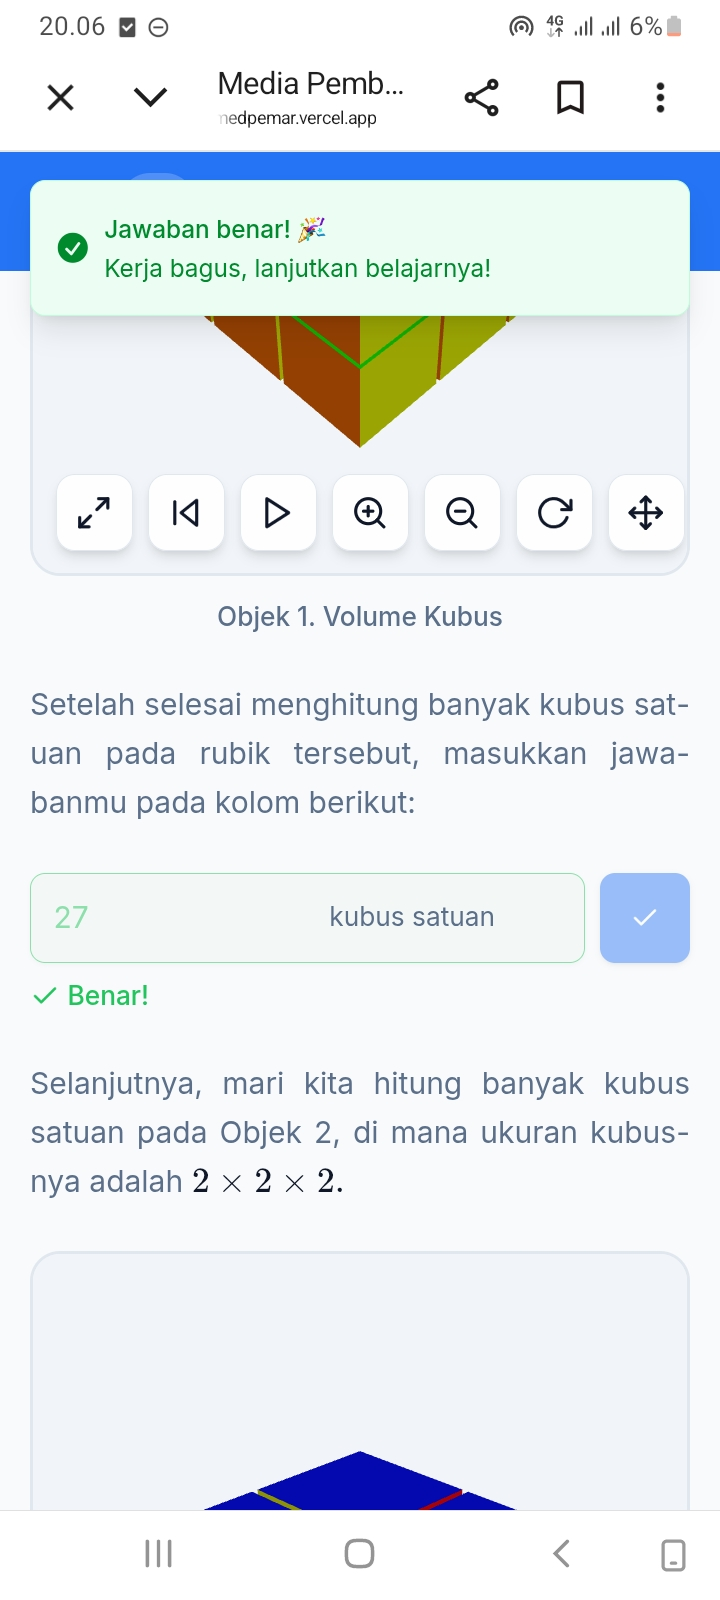
\includegraphics[width=0.3\textwidth]{images2/isiansingkat.jpg}
            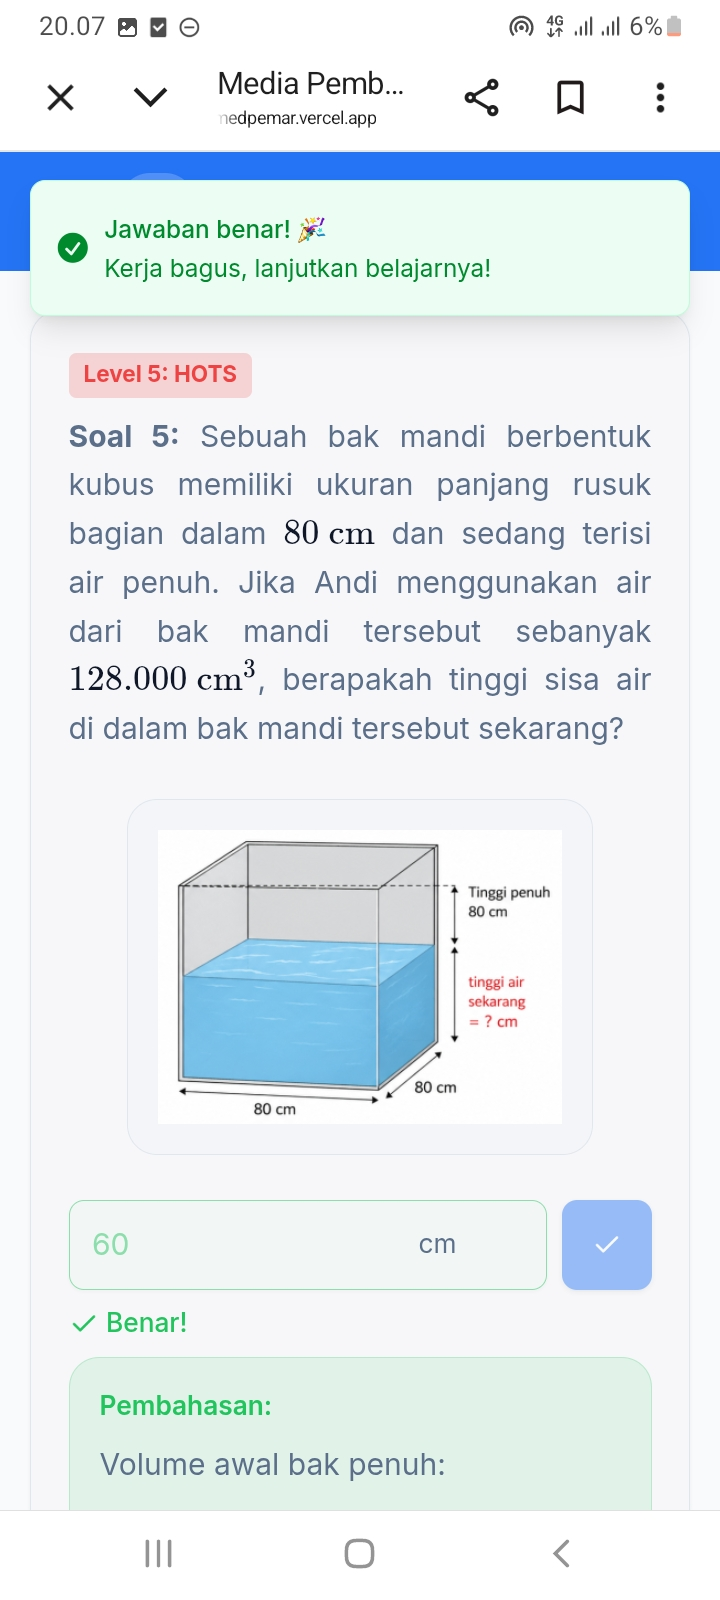
\includegraphics[width=0.3\textwidth]{images2/soalakhirbab.jpg}
            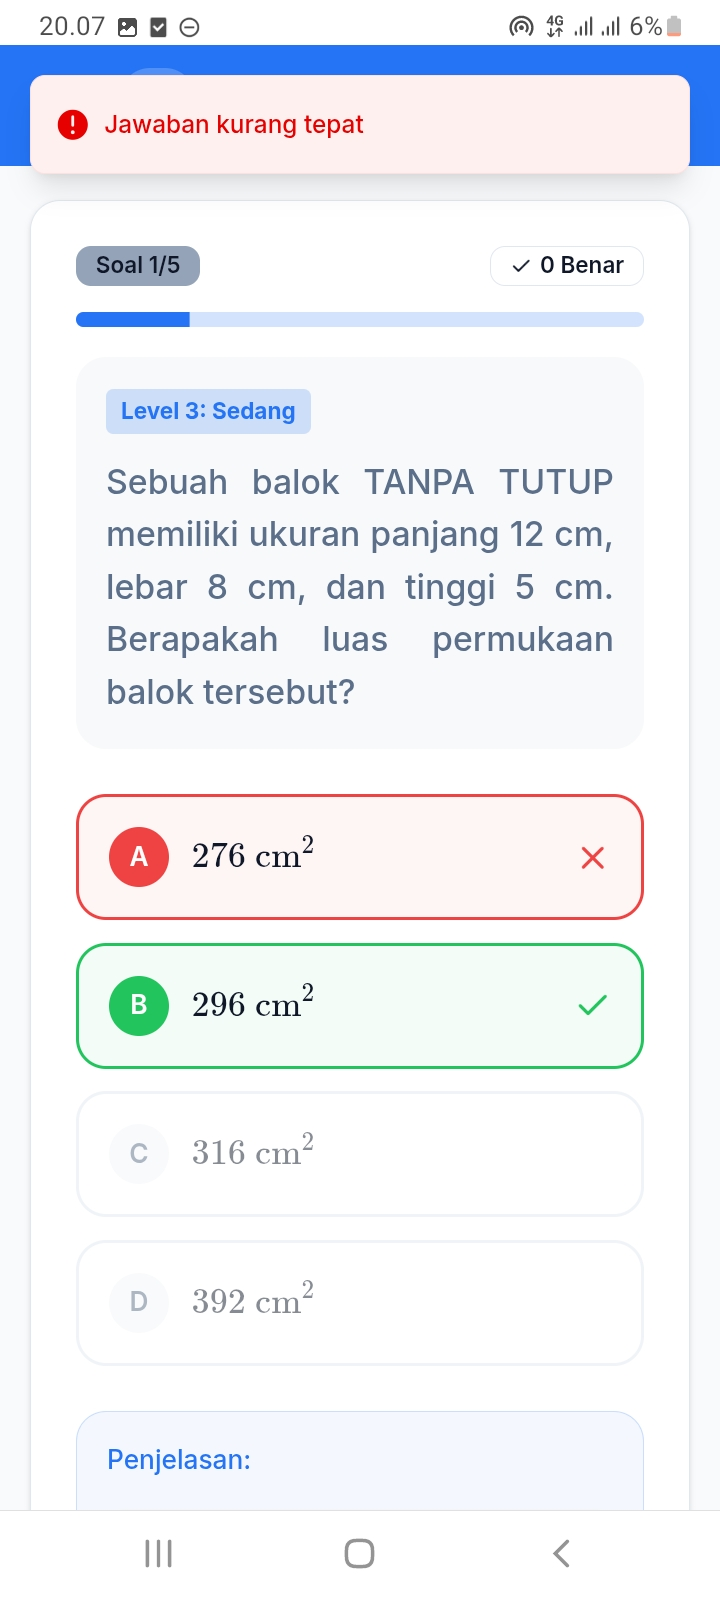
\includegraphics[width=0.3\textwidth]{images2/quizvolume.jpg}
            \caption{Contoh Soal Evaluasi}
            \label{fig:contohsoalevaluasi}
        \end{figure}
        \item Integrasi Sistem\\
        \hspace*{1cm}Integrasi sistem melibatkan penggabungan semua komponen pengembangan menjadi satu aplikasi yang kohesif. Model 3D dari Blender diintegrasikan ke dalam komponen React melalui Three.js. Konten 2D dari GeoGebra diimpor sebagai aset gambar. Sistem penyimpanan aset menggunakan Supabase Storage, dan aplikasi React dikonfigurasi untuk mengambil aset dari URL yang disediakan. Testing dilakukan untuk memastikan semua komponen bekerja bersama tanpa eror dan performa aplikasi optimal.

        
        \item Validasi Produk\\
        \hspace*{1cm}Validasi produk dilakukan oleh tim ahli materi dan ahli media untuk memastikan kelayakan media pembelajaran dari berbagai aspek sebelum pengujian lapangan. Proses validasi ini bertujuan untuk mengidentifikasi kekurangan, mendapatkan kritik, saran, dan penilaian konstruktif yang dijadikan acuan untuk perbaikan produk.
        
        \textbf{Validasi Ahli Materi:}
        
        \hspace*{1cm}Validasi konten materi dilakukan oleh dua ahli materi:
        \begin{enumerate}[leftmargin=*, label=--]
            \item Ibu Rima Aksen Cahdriyana, M.Pd., dosen Pendidikan Matematika Universitas Ahmad Dahlan (UAD).
            \item Bapak Wibowo Ramadhiyanto, S.Pd., pendidik Matematika SMP Muhammadiyah 9 Yogyakarta.
        \end{enumerate}
        
        \hspace*{1cm}Tujuan validasi ahli materi adalah untuk memperoleh kritik, saran, dan penilaian terhadap keakuratan konten matematika, kesesuaian dengan capaian pembelajaran kurikulum, dan kelayakan materi untuk dipelajari melalui media simulasi 3D. Saran, masukan, dan tindak lanjut dari ahli materi disajikan pada Tabel \ref{tabel:validasimateri} berikut.
        \begin{table}[H]
\begin{adjustwidth}{-2cm}{-2cm}
    \centering
    \caption{Saran, Masukan, dan Tindak Lanjut Validasi Ahli Materi}
    \label{tabel:validasimateri}
    \begin{tabular}{|c|p{9cm}|c|}
        \hline
        \textbf{No} & \textbf{Saran dan Masukan} & \textbf{Tindak Lanjut} \\
        \hline
        1 & Perlu penambahan kata "satuan" pada kolom input kubus satuan. & Sudah direvisi \\
        \hline
        2 & Kalimat "kubus tersebut tidak terbentuk dari kubus satuan" kurang tepat secara konsep, karena pada dasarnya setiap kubus dapat dipandang tersusun dari kubus satuan, meskipun tidak ditampilkan secara eksplisit. Oleh karena itu, kalimat tersebut sebaiknya diubah menjadi "tidak ditampilkan dalam bentuk kubus satuan". & Sudah direvisi \\
        \hline
        3 & Penggunaan istilah "representasi" kurang sesuai untuk siswa SMP. Disarankan untuk mengganti dengan kalimat yang lebih sederhana, seperti "banyaknya kubus satuan yang menyusun suatu kubus menunjukkan volume kubus tersebut". & Sudah direvisi \\
        \hline
        4 & Definisi prisma perlu diperbaiki karena berpotensi menimbulkan kebingungan bagi siswa. & Sudah direvisi \\
        \hline
        5 & Perlu penambahan satu paragraf pengantar sebelum definisi jaring-jaring. Contohnya: "Perhatikan kardus pada gambar di atas. Kardus tersebut berbentuk kubus. Untuk menghitung luas permukaan kubus, diperlukan luas seluruh sisi. Salah satu cara untuk melihat seluruh sisi kubus adalah dengan membukanya menjadi jaring-jaring," kemudian dilanjutkan dengan definisi jaring-jaring. & Sudah direvisi \\
        \hline
        6 & Memperbanyak variasi jaring-jaring prisma. & Sudah direvisi \\
        \hline
        7 & Menambahkan Capaian Pembelajaran, Tujuan Pembelajaran, dan Indikator Pencapaian Kompetensi di bagian awal website. & Sudah direvisi \\
        \hline
    \end{tabular}
\end{adjustwidth}
\end{table}
\newpage
        
        \textbf{Validasi Ahli Media:}
        
        \hspace*{1cm}Validasi aspek media dilakukan oleh dua ahli media:
        \begin{enumerate}[leftmargin=*, label=--]
            \item Bapak Anggit Prabowo, M.Pd., dosen Pendidikan Matematika Universitas Ahmad Dahlan (UAD).
            \item Bapak Wibowo Ramadhiyanto, S.Pd., pendidik Matematika SMP Muhammadiyah 9 Yogyakarta.
        \end{enumerate}
        
        \hspace*{1cm}Validasi ahli media bertujuan untuk menilai kualitas kegrafikan, kelayakan bahasa, dan kualitas perangkat lunak. Tidak ada revisi yang signifikan dari kedua validator. Hanya saja ada kunci jawaban soal yang salah dan sudah direvisi. Bapak Wibowo menyampaikan bahwa media pembelajaran memiliki visual yang baik, serta terdapat ilustrasi yang dapat mempermudah pemahaman peserta didik.

    \end{enumerate}

    \item \textbf{Implementasi}\\
    \hspace*{1cm}Pada tahap implementasi ini, peneliti melakukan uji coba terhadap produk yang telah dikembangkan. Uji coba dilakukan terhadap peserta didik kelas VIII-B dan VIII-D SMP Muhammadiyah 9 Yogyakarta. Tahap ini bertujuan untuk memperoleh informasi mengenai kelayakan media pembelajaran yang telah dikembangkan. Pada tahap ini, terdapat dua jenis uji coba yang dilakukan, yaitu uji coba kelas kecil dan uji coba kelas besar. Berikut adalah penjelasan mengenai uji coba kelas kecil dan uji coba kelas besar.
    \begin{enumerate}
        \item Uji Coba Kelas Kecil \\
        \hspace*{1cm}Uji coba kelas kecil dilakukan pada tanggal 18 Mei 2026 dengan melibatkan 5 peserta didik kelas VIII-D yang dipilih secara acak. Kegiatan ini dilaksanakan melalui pembelajaran menggunakan media yang sedang dikembangkan. Setelah pembelajaran selesai, peserta didik diminta mengisi angket untuk mengetahui respons mereka terhadap media tersebut.

        \hspace*{1cm}Sebelum pelaksanaan, peneliti terlebih dahulu meminta izin kepada pendidik matematika kelas VIII-D. Pemilihan peserta didik dilakukan secara acak oleh pendidik. Selama uji coba, peserta didik menggunakan media pembelajaran dan kemudian mengisi angket penilaian.

        \hspace*{1cm}Hasil angket menunjukkan bahwa media pembelajaran memudahkan pemahaman materi, menarik, serta diharapkan dapat dikembangkan untuk materi lainnya. Pada tahap ini tidak terdapat saran revisi dari peserta didik, sehingga pengembangan dapat dilanjutkan ke tahap berikutnya.


        \item Uji Coba Kelas Besar \\
        \hspace*{1cm}Uji coba kelas besar dilakukan dengan melibatkan seluruh peserta didik kelas VIII-B SMP Muhammadiyah 9 Yogyakarta pada tanggal 20 Mei 2026. Pemilihan kelas tersebut didasarkan pada rekomendasi pendidik matematika karena pendidik tersebut mengampu kelas tersebut dan materi bangun ruang sedang diajarkan.

        \hspace{1cm}Pelaksanaan uji coba dilakukan melalui pembelajaran menggunakan media pembelajaran berbasis simulasi 3D. Setelah pembelajaran selesai, peserta didik diminta mengisi angket yang telah disiapkan. Angket tersebut digunakan untuk memperoleh penilaian peserta didik terhadap kualitas media pembelajaran yang dikembangkan. Peserta didik menyampaikan bahwa materi mudah dipahami dan pembelajaran menjadi tidak membosankan. Mereka juga menyarankan agar tidak terlalu banyak bacaan dan contoh soal diperbanyak.
    \end{enumerate}

    \item \textbf{Evaluasi}
    
    \hspace{1cm}Tahap evaluasi merupakan tahap akhir dalam model pengembangan ADDIE. Evaluasi dilakukan untuk menganalisis hasil uji coba terhadap media pembelajaran berbasis simulasi 3D pada materi bangun ruang sisi datar kelas VIII. Tujuan dari tahap ini adalah untuk menyempurnakan produk yang telah dikembangkan sebelum menghasilkan produk akhir yang layak digunakan. Selanjutnya, dilakukan revisi akhir berdasarkan masukan dari ahli materi, ahli media, dan peserta didik.

    \hspace{1cm}Berdasarkan hasil validasi dari ahli materi dan ahli media, terdapat beberapa masukan terhadap media pembelajaran yang dikembangkan sebelum dilakukan uji coba kepada peserta didik. Selanjutnya, dilakukan revisi berdasarkan masukan tersebut hingga media pembelajaran masuk dalam kategori baik atau dinyatakan layak. Evaluasi yang dilakukan mencakup hasil validasi dari ahli materi dan ahli media, serta angket hasil uji coba media oleh peserta didik. Penilaian tersebut dijadikan acuan dalam menentukan kelayakan media pembelajaran yang dikembangkan.

\end{enumerate}
% ANALISIS DATA
\textbf{B. Analisis Data}
\addcontentsline{toc}{section}{B. Analisis Data}

\hspace{1cm}Analisis data merupakan tahap lanjutan dari tahap evaluasi dalam model pengembangan ADDIE. Data yang diperoleh dalam penelitian ini berupa data kualitatif yang kemudian dikonversi menjadi data kuantitatif. Analisis data dilakukan berdasarkan lembar penilaian dari ahli materi, ahli media, dan respons peserta didik. Media pembelajaran yang dikembangkan dinyatakan layak apabila memperoleh skor rata-rata penilaian dari ahli materi, ahli media, dan respons peserta didik minimal pada kategori "Baik". Berikut ini adalah hasil analisis data tersebut:
\begin{enumerate}
    \item Analisis Penilaian Angket Ahli Materi\\
    \hspace*{1cm}Validasi oleh ahli materi dilakukan untuk memperoleh penilaian berupa skor, komentar, dan masukan terhadap materi yang telah dikembangkan dalam media pembelajaran berbasis simulasi 3D. Komentar dan saran dari validator digunakan untuk menyempurnakan media pembelajaran agar menghasilkan produk akhir yang layak digunakan. Kelayakan materi dalam media pembelajaran ini dinilai oleh dua orang ahli, yaitu Ibu Rima Aksen Cahdriyana, M.Pd., dosen Pendidikan Matematika UAD sebagai validator 1, dan Bapak Wibowo Ramadhiyanto, S.Pd., pendidik Matematika di SMP Muhammadiyah 9 Yogyakarta, sebagai validator 2. Hasil penilaian kelayakan media pembelajaran disajikan pada Tabel \ref{penilaianmateri}.
    \begin{table}[H]
        \begin{adjustwidth}{-2cm}{-2cm}
            \centering
            \caption{Hasil Penilaian Materi Pembelajaran Berdasarkan Aspek Penilaian}
            \label{penilaianmateri}
            \begin{tabular}{|l|c|c|c|l|}
                \hline
                \textbf{Aspek} & \textbf{Validator 1} & \textbf{Validator 2} & \textbf{Rata-rata Skor} & \textbf{Kategori Kualitatif}\\
                \hline
                Aspek Isi & \(4\) & \(4{,}71\) & \(4{,}35\) & Sangat Baik\\
                Aspek Bahasa & \(4\) & 5 & \(4{,}5\) & Sangat Baik\\
                Aspek Penyajian & \(4{,}5\) & \(4{,}87\) & \(4{,}68\) & Sangat Baik\\
                Aspek Simulasi 3D & \(5\) & 5 & 5 & Sangat Baik\\
                \hline
                \multicolumn{3}{|c|}{Kesimpulan} & \(4{,}63\) & Sangat Baik\\
                \hline
            \end{tabular}
        \end{adjustwidth}
    \end{table}
    % \begin{table}[H]
    %     \begin{adjustwidth}{-2cm}{-2cm}
    %         \centering
    %         \caption{Hasil Penilaian Media Pembelajaran Menurut Ahli Media}
    %         \label{penilaianmateri}
    %         \begin{tabular}{|c|c|c|c|c|c|}
    %             \hline
    %             \textbf{No} & \textbf{Validator} & \textbf{Skor} & \textbf{Rata-rata Skor} & \textbf{Kriteria Data Kuantitatif}\\
    %             \hline
    %             1 & Rima Aksen Cahdriyana, M.Pd. & 0 & 0 & Sangat Baik\\
    %             2 & Wibowo Ramadhiyanto, S.Pd. & 0 & 0 & Sangat Baik\\
    %             \hline
    %             \multicolumn{2}{|c|}{Jumlah Skor} & 0 & & \\
    %             \hline
    %             \multicolumn{2}{|c|}{Rata-rata Keseluruhan} & 0 & 0 & Sangat Baik\\
    %             \hline
    %         \end{tabular}
    %     \end{adjustwidth}
    % \end{table}

    \begin{table}[H]
        \centering
        \caption{Kriteria Penilaian Ahli Materi, Ahli Media, dan Respons Peserta Didik}
        \label{tab:kriteriaahli}
        \begin{tabular}{|c|c|l|}
            \hline
            \textbf{No} & \textbf{Rentang Skor \( (i) \) Kuantitatif} & \textbf{Kategori Kualitatif}\\
            \hline
            1 & \( \bar{x} > 4{,}2 \) & Sangat Baik\\
            2 & \( 3{,}4 < \bar{x} \leq 4{,}2 \) & Baik\\
            3 & \( 2{,}6 < \bar{x} \leq 3{,}4 \) & Cukup Baik\\
            4 & \( 1{,}8 < \bar{x} \leq 2{,}6 \) & Kurang\\
            5 & \( \bar{x} \leq 1{,8} \) & Sangat Kurang\\
            \hline 
        \end{tabular}
    \end{table}
    \hspace*{1cm}Dari Tabel \ref{penilaianmateri} diperoleh skor rata-rata penilaian kedua validator sebesar \(4{,}63\). Mengacu pada kriteria penilaian yang ditetapkan pada Tabel \ref{tab:kriteriaahli}, skor sebesar \(4{,}63\) berada di atas nilai ambang batas \(\bar{x} > 4{,}2\), sehingga termasuk dalam kategori \textbf{Sangat Baik}. Selain itu, kedua validator juga memberikan skor penuh sebesar 5 pada aspek simulasi 3D, yang menunjukkan bahwa penggunaan simulasi 3D dalam media pembelajaran mendapat respons yang sangat positif.

    \item Analisis Penilaian Angket Ahli Media\\
    \hspace*{1cm}Validasi oleh ahli media dilakukan untuk memperoleh penilaian berupa skor, komentar, dan masukan terhadap media pembelajaran yang dikembangkan. Komentar dan saran dari validator media digunakan untuk menyempurnakan media pembelajaran agar menghasilkan produk akhir yang layak digunakan. Kelayakan media pembelajaran ini dinilai oleh dua orang ahli media, yaitu Bapak Anggit Prabowo, M.Pd., dosen Pendidikan Matematika UAD sebagai validator 1, dan Bapak Wibowo Ramadhiyanto, S.Pd., pendidik Matematika di SMP Muhammadiyah 9 Yogyakarta sebagai validator 2. Hasil penilaian kelayakan oleh ahli media disajikan pada Tabel~\ref{penilaianmedia}.
    \begin{table}[H]
        \begin{adjustwidth}{-2cm}{-2cm}
            \centering
            \caption{Hasil Penilaian Media Pembelajaran Berdasarkan Aspek Penilaian}
            \label{penilaianmedia}
            \begin{tabular}{|l|c|c|c|l|}
                \hline
                \textbf{Aspek} & \textbf{Validator 1} & \textbf{Validator 2} & \textbf{Rata-rata Skor} & \textbf{Kategori Kualitatif}\\
                \hline
                Kualitas Kegrafikan & \(4{,}33\) & \(4{,}91\) & \(4{,}62\) & Sangat Baik\\
                Kelayakan Bahasa & \(4{,}33\) & \(4{,}75\) & \(4{,}54\) & Sangat Baik\\
                Kualitas Perangkat Lunak & \(4{,}66\) & \(5\) & \(4{,}83\) & Sangat Baik\\
                \hline
                \multicolumn{3}{|c|}{Kesimpulan} & \(4{,}66\) & Sangat Baik\\
                \hline
            \end{tabular}
        \end{adjustwidth}
    \end{table}

    % \begin{table}[H]
    %     \centering
    %     \caption{Kriteria Penilaian Ahli Media}
    %     \begin{tabular}{|c|c|c|}
    %         \hline
    %         \textbf{No} & \textbf{Rentang Skor \( (i) \) Kuantitatif} & \textbf{Kategori Kualitatif}\\
    %         \hline
    %         1 & \( \bar{x} > 4{,}21 \) & Sangat Baik\\
    %         2 & \( 3{,}41 < \bar{x} \leq 4{,}2 \) & Baik\\
    %         3 & \( 2{,}60 < \bar{x} \leq 3{,}41 \) & Cukup Baik\\
    %         4 & \( 1{,}80 < \bar{x} \leq 2{,}60 \) & Kurang\\
    %         5 & \( \bar{x} \leq 1{,80} \) & Sangat Kurang\\
    %         \hline 
    %     \end{tabular}
    % \end{table}
    \hspace*{1cm}Dari Tabel \ref{penilaianmedia} diperoleh skor rata-rata penilaian kedua validator sebesar \(4{,}66\). Mengacu pada kriteria penilaian yang ditetapkan pada Tabel \ref{tab:kriteriaahli}, skor sebesar \(4{,}66\) berada di atas nilai ambang batas \(\bar{x} > 4{,}2\), sehingga termasuk dalam kategori \textbf{Sangat Baik}. Selain itu, kedua validator juga memberikan skor tinggi pada aspek kualitas perangkat lunak, dengan skor rata-rata sebesar \(4{,}83\), yang menunjukkan bahwa media pembelajaran berbasis simulasi 3D yang dikembangkan memiliki kualitas perangkat lunak yang sangat baik.

    \item Analisis Penilaian Angket Respons Peserta Didik\\
    \hspace*{1cm}Respons peserta didik diperoleh melalui uji coba kelas kecil dan uji coba kelas besar yang bertujuan untuk mendapatkan penilaian berupa skor, komentar, dan masukan terhadap media pembelajaran yang telah dikembangkan. Respons tersebut dianalisis berdasarkan hasil angket yang disebarkan kepada peserta didik kelas VIII-B SMP Muhammadiyah 9 Yogyakarta. Kriteria penilaian angket respons peserta didik disajikan pada Tabel \ref{tab:kriteriaahli}. Kriteria ini mengacu pada buku Prof. Sugiyono 2019 tentang metode penelitian kuantitatif, kualitatif, dan R\&D. Adapun hasil uji coba kelas kecil disajikan pada Tabel~\ref{ujikelaskecil}.

    \begin{table}[H]
        \centering
        \caption{Data Hasil Ujicoba Kelas Kecil}
        \label{ujikelaskecil}
        \begin{tabular}{|c|l|c|l|}
            \hline
            \textbf{No} & \textbf{Nama} & \textbf{Rata-rata Skor} & \textbf{Kategori Kualitatif} \\
            \hline
            1 & Gilang Affan A. & \(4{,}35\) & Sangat Baik \\
            2 & Rachma Riski & \(4{,}85\) & Sangat Baik \\
            3 & Alif Bagas P. & \(4{,}15\) & Baik \\
            4 & Jasmine Sekar C. A. & \(3{,}38\) & Cukup Baik \\
            5 & Meydita Maharani & \(4{,}85\) & Sangat Baik \\
            \hline
            \multicolumn{2}{|c|}{Rata-rata Kelas Kecil} & \(4{,}31\) & Sangat Baik \\
            \hline
        \end{tabular}
    \end{table}
    Hasil uji coba kelas kecil menunjukkan bahwa skor rata-rata respons peserta didik sebesar \(4{,}31\). Mengacu pada kriteria penilaian yang ditetapkan pada Tabel \ref{tab:kriteriaahli}, skor sebesar \(4{,}31\) berada di atas nilai ambang batas \(\bar{x} > 4{,}2\), sehingga termasuk dalam kategori \textbf{Sangat Baik}. Peserta didik memberikan tanggapan bahwa media pembelajaran ini menarik, mudah dipahami, dan menyarankan untuk diterapkan pada materi pembelajaran lain. Dari hasil ini, tidak terdapat rekomendasi revisi yang signifikan untuk produk berdasarkan uji coba kelas kecil, sehingga bisa langsung dilanjutkan ke tahap uji coba kelas besar.\\
    % \begin{figure}[H]
    %     \centering
    %     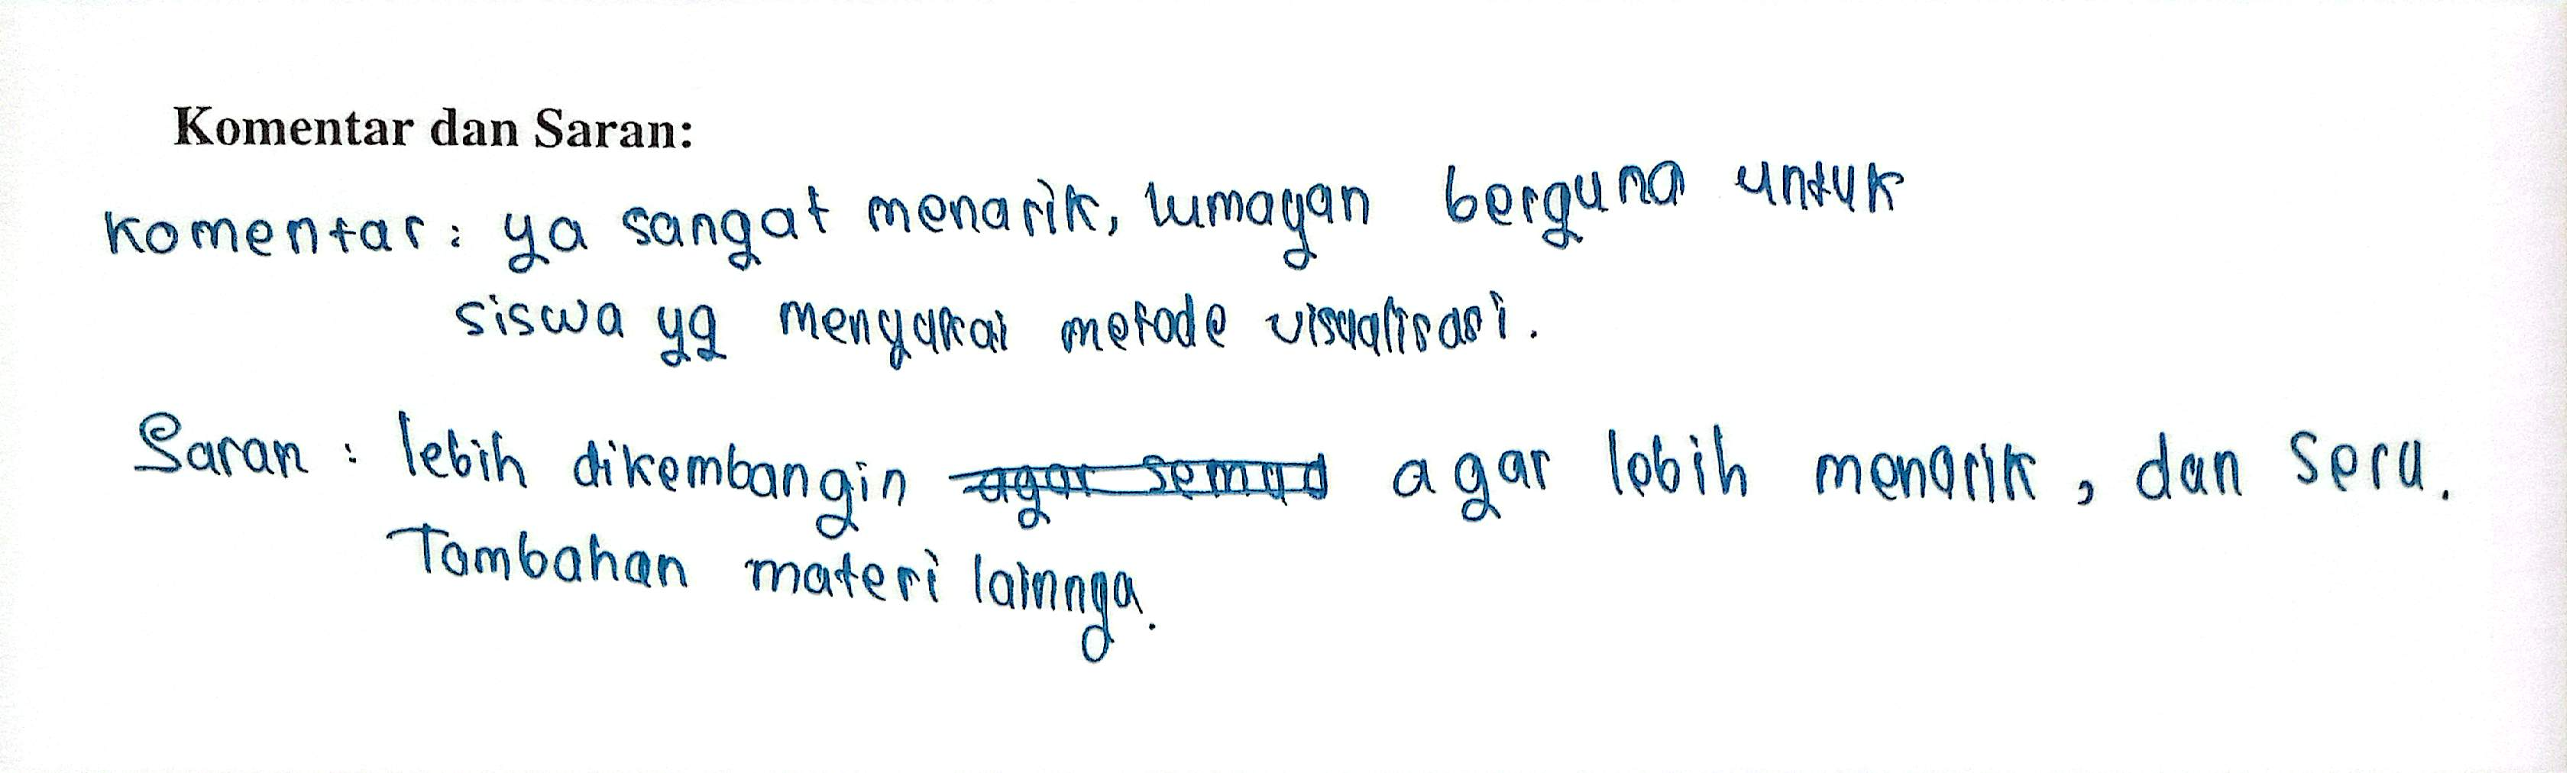
\includegraphics[width=1\textwidth]{komentar/kelaskecil1.jpg}
    %     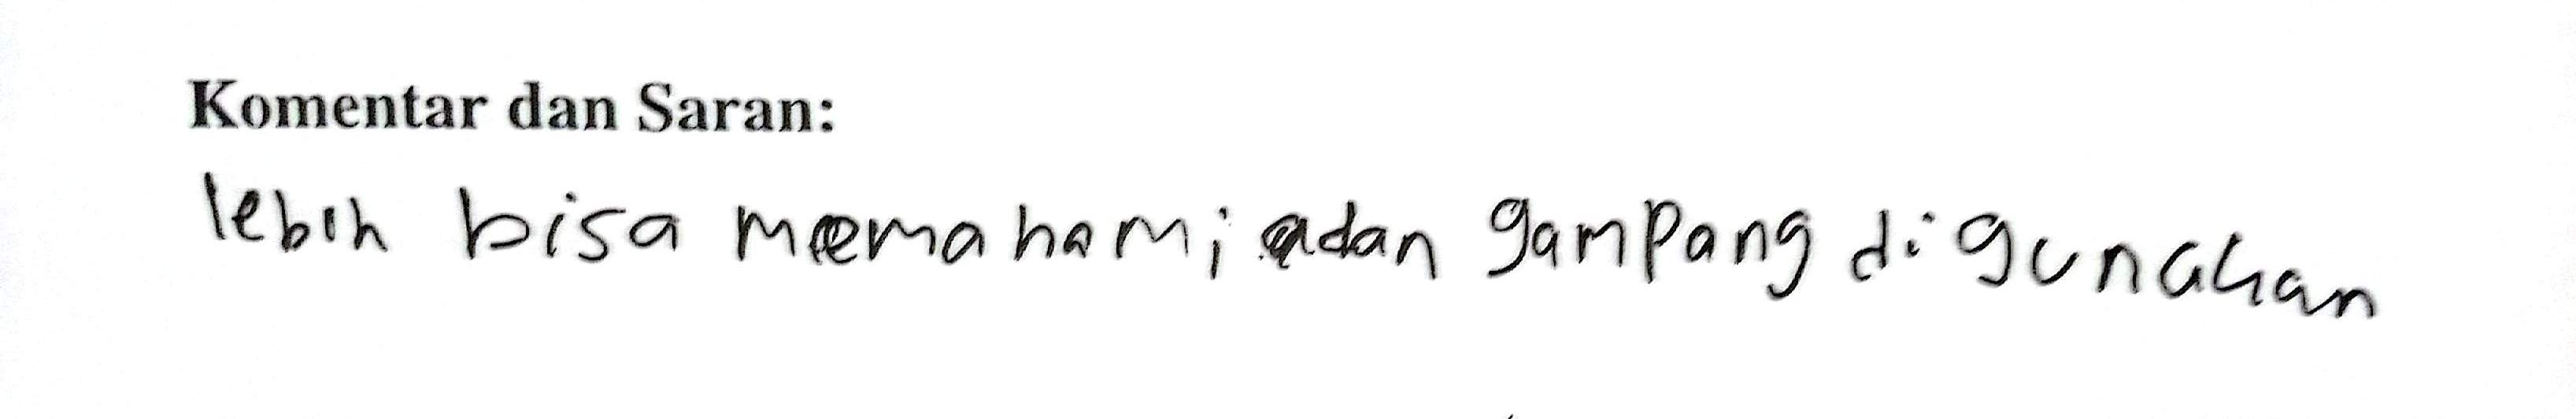
\includegraphics[width=1\textwidth]{komentar/kelaskecil2.jpg}
    %     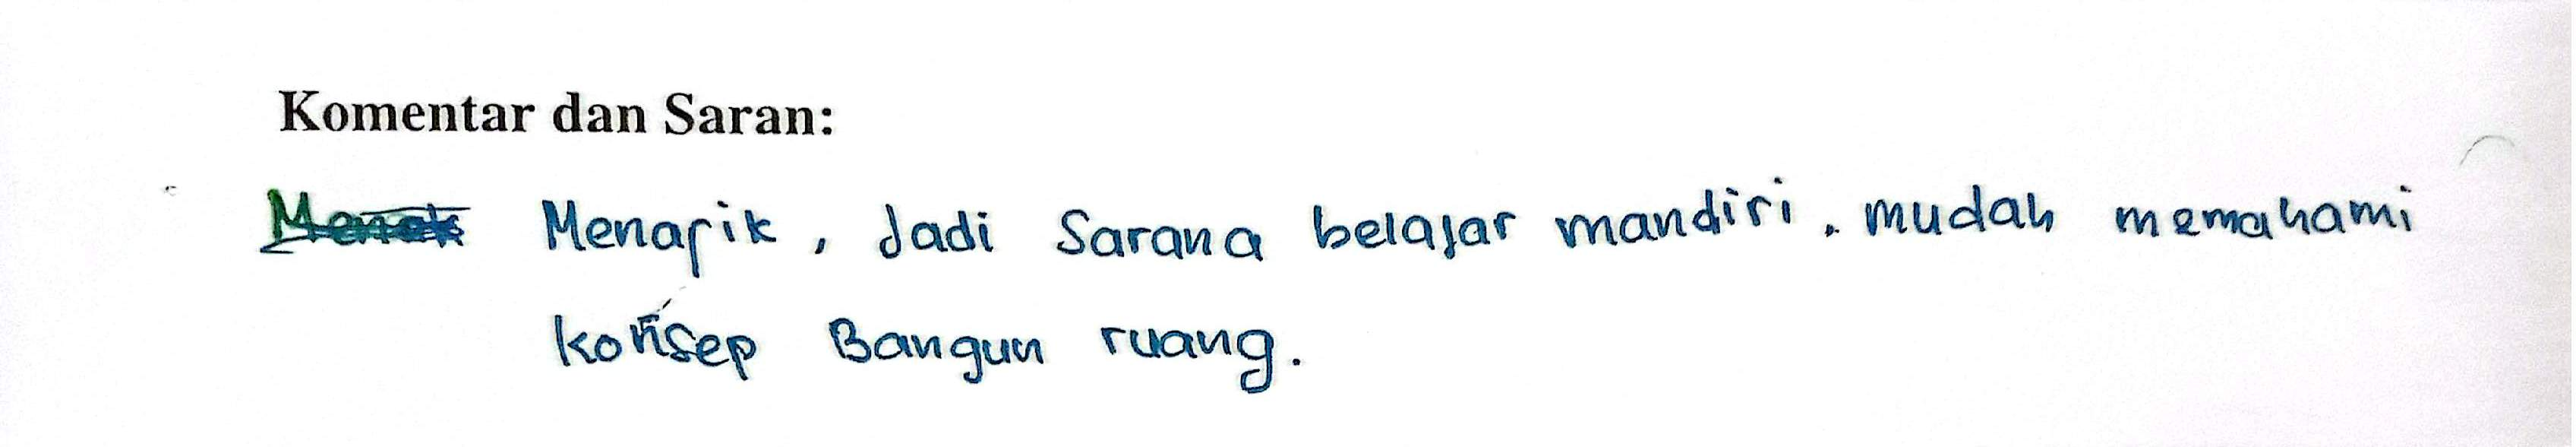
\includegraphics[width=1\textwidth]{komentar/kelaskecil3.jpg}
    %     \caption{Komentar dan Saran Kelas Kecil}
    %     \label{saran1}
    % \end{figure}
    \hspace*{1cm}Berdasarkan pengambilan data pada uji coba kelas besar yang melibatkan 21 peserta didik kelas VIII-B, diperoleh hasil seperti pada Tabel \ref{ujikelasbesar}.
    \begin{table}[H]
        \centering
        \caption{Data Hasil Ujicoba Kelas Besar}
        \label{ujikelasbesar}
        \begin{tabular}{|c|l|c|l|}
            \hline
            \textbf{No} & \textbf{Nama} & \textbf{Rata-rata Skor} & \textbf{Kategori Kualitatif} \\
            \hline
            1 & Athayya Anindya & \(4{,}96\) & Sangat Baik \\
            2 & Dimas Galih M. & \(4{,}62\) & Sangat Baik \\
            3 & Arletta Prada R. & \(4{,}96\) & Sangat Baik \\
            4 & Sinayang Kusuma N. & \(4{,}96\) & Sangat Baik \\
            5 & Zahra Nurlinda & \(4{,}88\) & Sangat Baik \\
            6 & Faiza Putri & \(4{,}92\) & Sangat Baik \\
            7 & Arawinda Putri A. & \(4{,}88\) & Sangat Baik \\
            8 & Kaffa Naura Kanifda & \(4{,}08\) & Baik \\
            9 & Daffa Raqillarafa & \(4{,}15\) & Baik \\
            10 & Tri Rui & \(4{,}35\) & Sangat Baik \\
            11 & Sandika Saputra & \(4{,}77\) & Sangat Baik \\
            12 & Chyntia Azzahra A. & \(5\) & Sangat Baik \\
            13 & Itsya Rama M. & \(4{,}62\) & Sangat Baik \\
            14 & Ilham & \(4{,}35\) & Sangat Baik \\
            15 & Adinda Kamelia & \(4{,}19\) & Baik \\
            16 & Rafa Abiyu S. & \(4{,}65\) & Sangat Baik \\
            17 & Callysta & \(4{,}96\) & Sangat Baik \\
            18 & Vaneza Aullisya L. & \(4{,}04\) & Baik \\
            19 & M. Isakhan Amir & \(4{,}58\) & Sangat Baik \\
            20 & Ibrahim Putra M. & \(5\) & Sangat Baik \\
            21 & Daffa Prakoso & \(4{,}73\) & Sangat Baik \\
            \hline
            \multicolumn{2}{|c|}{Rata-rata Kelas Besar} & \(4{,}65\) & Sangat Baik \\
            \hline
        \end{tabular}
    \end{table}
    Hasil uji coba kelas besar menunjukkan bahwa skor rata-rata respons peserta didik sebesar \(4{,}65\). Mengacu pada kriteria penilaian yang ditetapkan pada Tabel \ref{tab:kriteriaahli}, skor sebesar \(4{,}65\) berada di atas nilai ambang batas \(\bar{x} > 4{,}2\), sehingga termasuk dalam kategori \textbf{Sangat Baik}. Peserta didik memberikan umpan balik positif, meliputi pernyataan bahwa materi mudah dipahami, media pembelajaran menarik, dan simulasi 3D dapat meningkatkan motivasi belajar. Meskipun demikian, beberapa peserta didik memberikan rekomendasi untuk menambah jumlah contoh soal dengan tujuan meningkatkan pemahaman konsep. Dokumentasi lengkap dari komentar dan saran peserta didik tersaji secara rinci dalam lampiran penelitian ini.
    \item Kualitas Produk Secara Keseluruhan\\
    \hspace*{1cm}Kualitas media pembelajaran secara keseluruhan dinilai berdasarkan skor rata-rata dari ahli materi, ahli media, uji coba kelas kecil, dan uji coba kelas besar. Hasil perhitungan rata-rata keseluruhan dari keempat penilaian tersebut disajikan pada Tabel~\ref{ratakeseluruhan}.\\
    \begin{table}[H]
        \centering
        \caption{Hasil Rata-rata Keseluruhan}
        \label{ratakeseluruhan}
        \begin{tabular}{|c|l|c|l|}
            \hline
            \textbf{No} & \textbf{Sampel Uji Coba} & \textbf{Rata-rata} & \textbf{Kategori Kualitatif}\\
            \hline
            1 & Ahli Materi & \(4{,}63\) & Sangat Baik\\
            2 & Ahli Media & \( 4{,}66 \) & Sangat Baik\\
            3 & Uji Coba Kelas Kecil & \(4{,}31\) & Sangat Baik\\
            4 & Uji Coba Kelas Besar & \( 4{,}65 \) & Sangat Baik\\
            \hline
            \multicolumn{2}{|c|}{Rata-rata Keseluruhan} & \(4{,}56\) & Sangat Baik\\
            \hline
            
        \end{tabular}
    \end{table}
    \hspace*{1cm}Berdasarkan hasil perhitungan rata-rata keseluruhan pada Tabel~\ref{ratakeseluruhan}, diperoleh skor rata-rata sebesar \(4{,}56\). Mengacu pada kriteria penilaian yang telah ditetapkan pada Tabel \ref{tab:kriteriaahli}, skor sebesar \(4{,}56\) berada di atas nilai ambang batas \(\bar{x} > 4{,}2\), sehingga termasuk dalam kategori \textbf{Sangat Baik}. Hasil ini menunjukkan bahwa media pembelajaran berbasis simulasi 3D yang dikembangkan memiliki kualitas yang sangat baik dan dinyatakan layak untuk digunakan dalam proses pembelajaran materi bangun ruang sisi datar untuk peserta didik kelas VIII.

\end{enumerate}
% REVISI PRODUK
\newpage
\textbf{C. Revisi Produk}
\addcontentsline{toc}{section}{C. Revisi Produk}

\hspace*{1cm}Revisi produk merupakan langkah penting dalam pengembangan media pembelajaran. Revisi dilakukan apabila masih terdapat kesalahan atau kekurangan pada produk yang dikembangkan. Pada tahap ini, peneliti melakukan revisi terhadap media pembelajaran berdasarkan saran dan masukan dari ahli materi dan ahli media. Adapun proses revisi dalam pengembangan media pembelajaran ini adalah sebagai berikut:
\begin{enumerate}
    \item Revisi Produk Hasil Validasi Ahli Materi\\
    \hspace*{1cm}Berdasarkan masukan dari ahli materi, perbaikan yang dilakukan telah sesuai dengan saran dan rekomendasi yang diberikan. Ahli materi memberikan masukan terkait beberapa definisi dan kosakata yang perlu dirubah, agar lebih mudah dimengerti oleh peserta didik. Selain itu ahli materi juga meminta untuk ditambah page yang isinya adalah Capaian Kompetensi, Tujuan Pembelajaran, dan Indikator Pencapaian Kompetensi. Hasil perbaikan tersebut disajikan sebagai berikut.
    \begin{enumerate}
        \item Menambahkan kata "satuan" dalam kolom input jawaban kubus satuan.
        \begin{table}[H]
            \centering
            \begin{tabular}{c c}
                Sebelum Revisi & Sesudah Revisi \\
                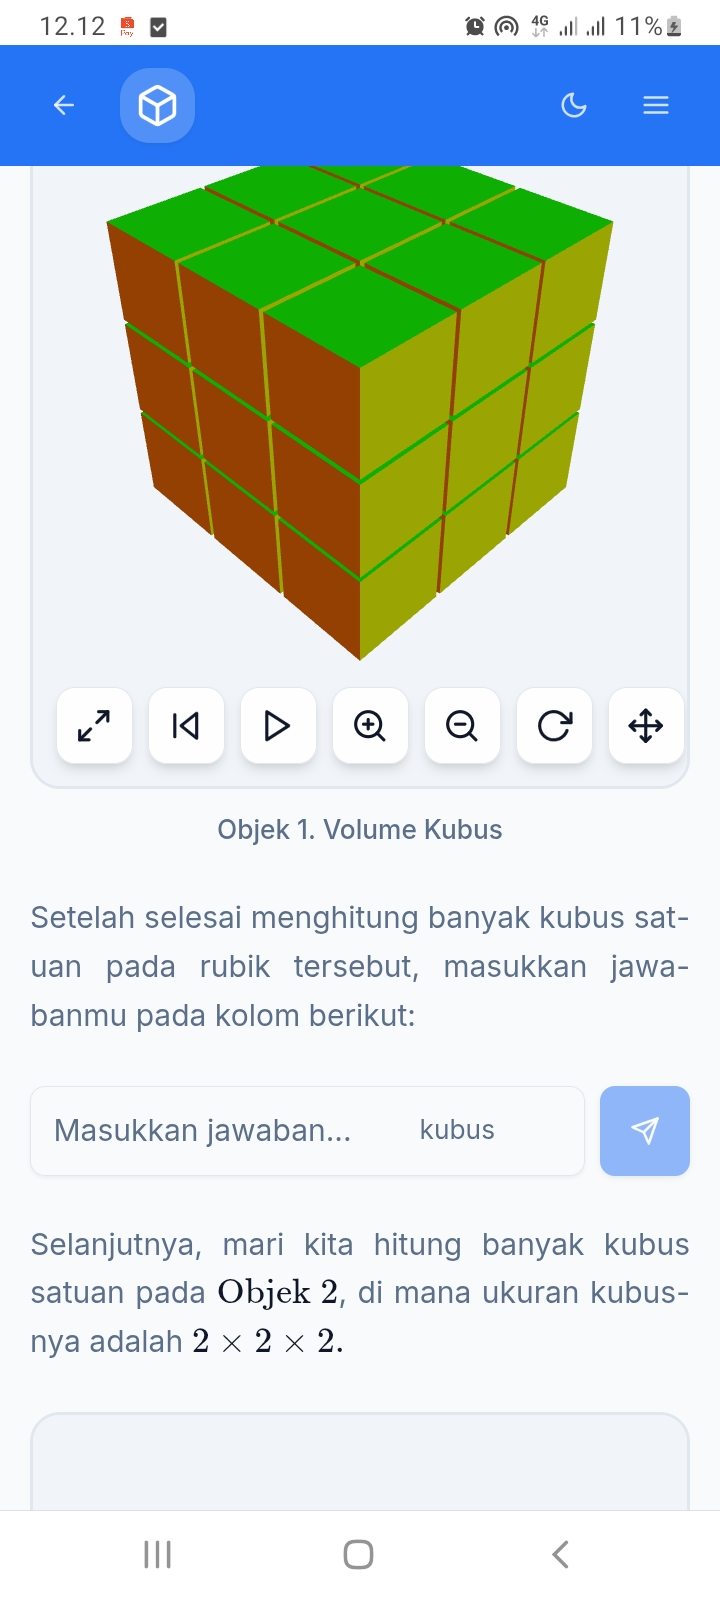
\includegraphics[width=0.25\textwidth]{revisi/sebelum/sebelumA.jpg} &
                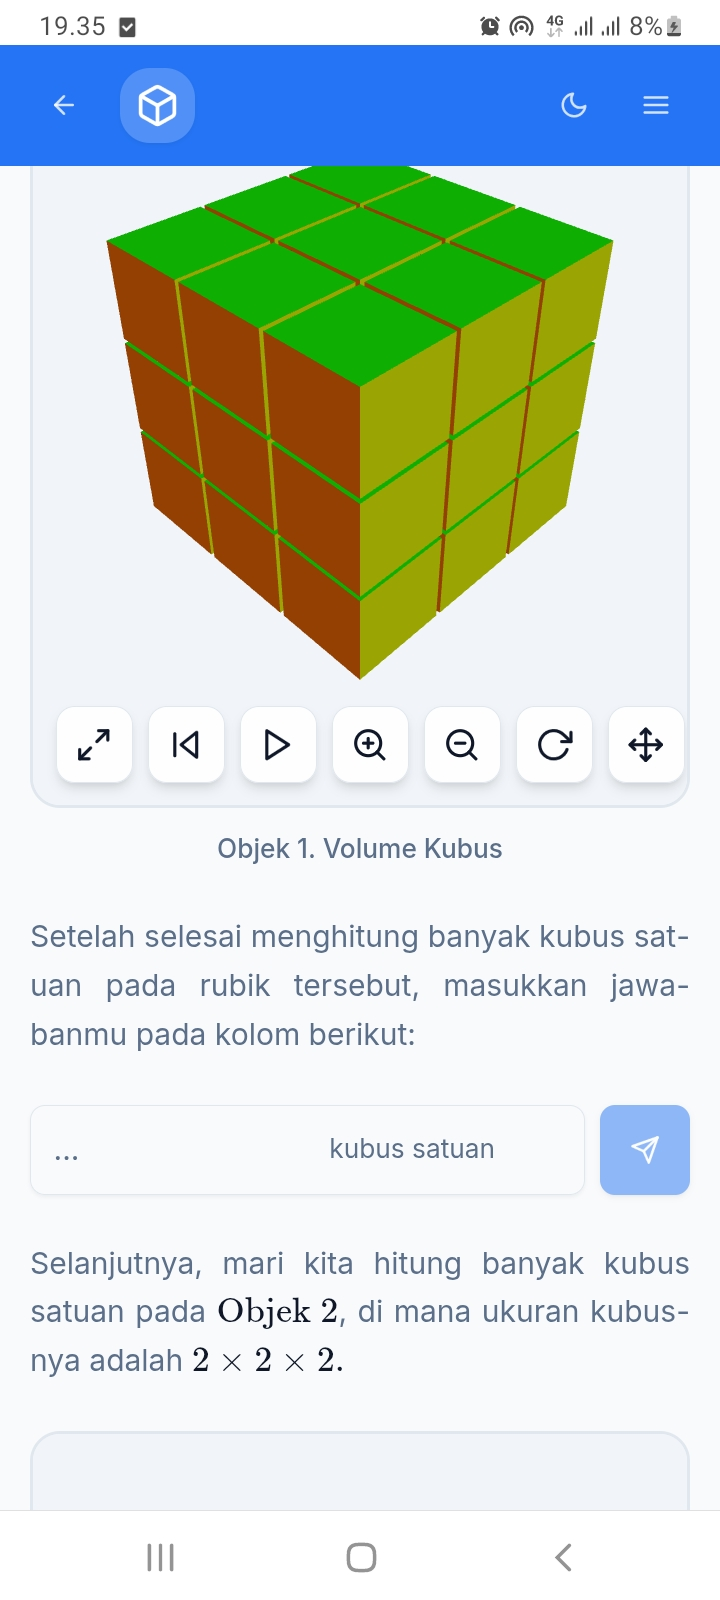
\includegraphics[width=0.25\textwidth]{revisi/sesudah/sesudahA.jpg} \\
            \end{tabular}
        \end{table}

        \item Memperbaiki definisi kubus yang kubus satuannya tidak ditampilkan.
        \begin{table}[H]
            \centering
            \begin{tabular}{c c}
                Sebelum Revisi & Sesudah Revisi \\
                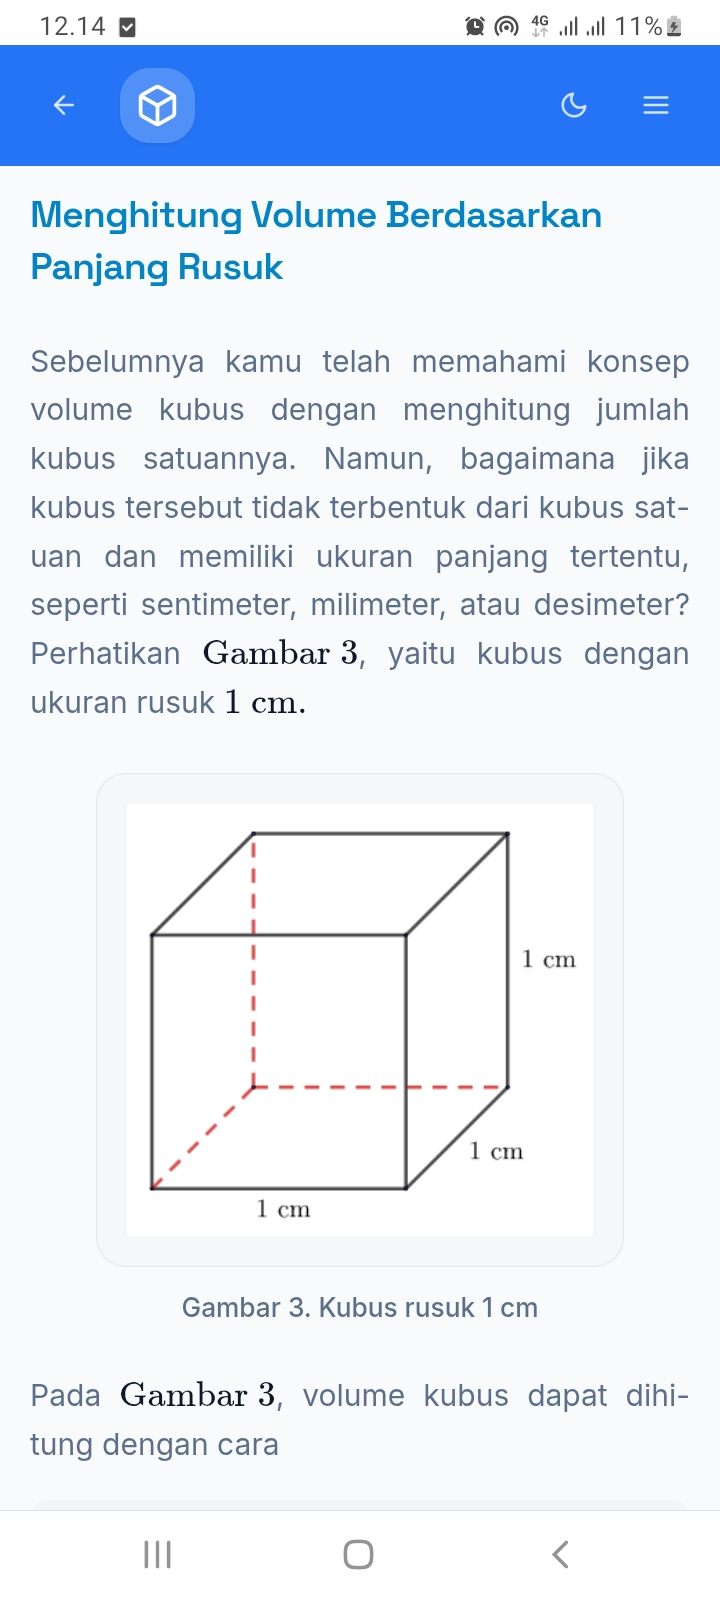
\includegraphics[width=0.25\textwidth]{revisi/sebelum/sebelumB.jpg} &
                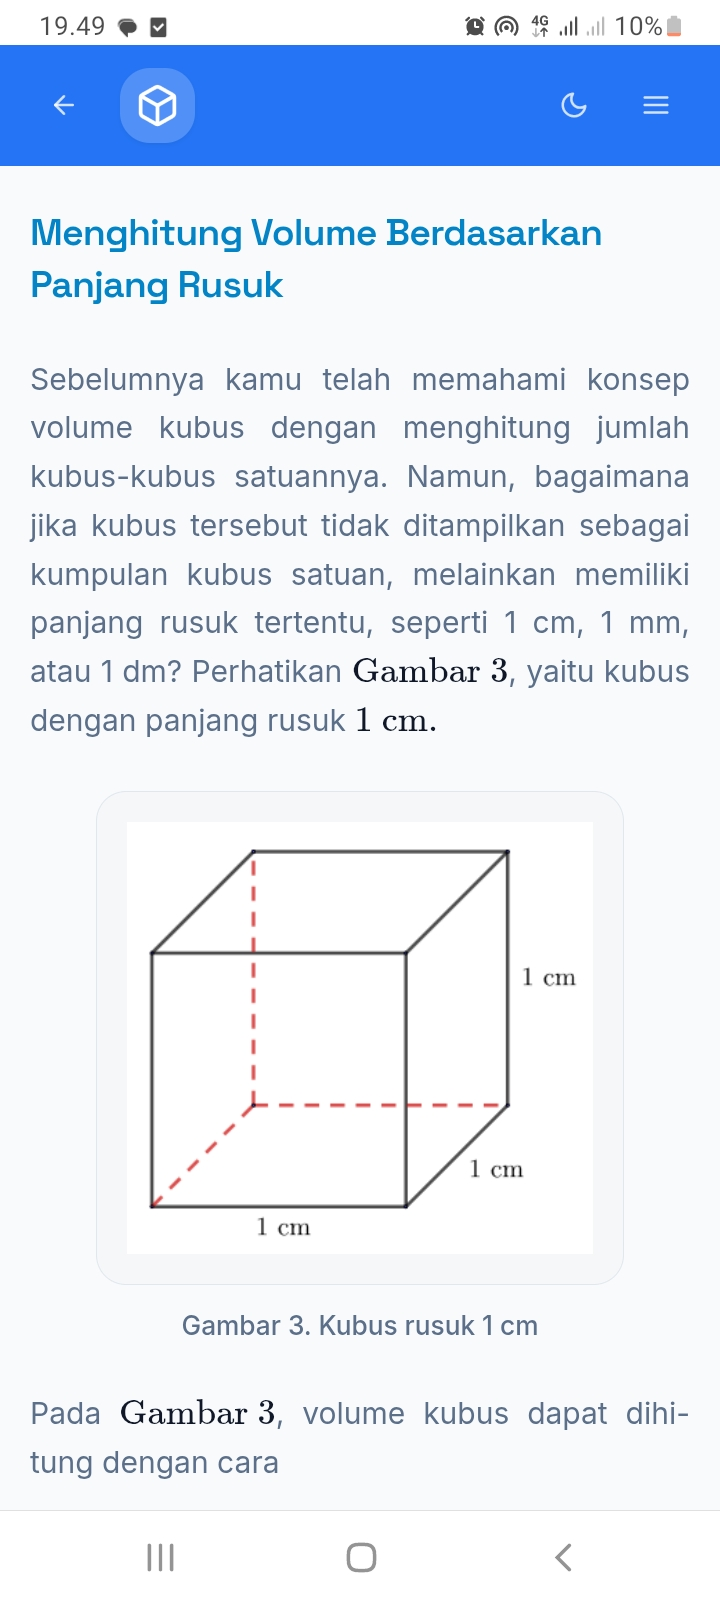
\includegraphics[width=0.25\textwidth]{revisi/sesudah/sesudahB.jpg} \\
            \end{tabular}
        \end{table}
        \item Mengganti kata "representasi" dengan kalimat yang mudah dipahami siswa SMP.
        \begin{table}[H]
            \centering
            \begin{tabular}{c c}
                Sebelum Revisi & Sesudah Revisi \\
                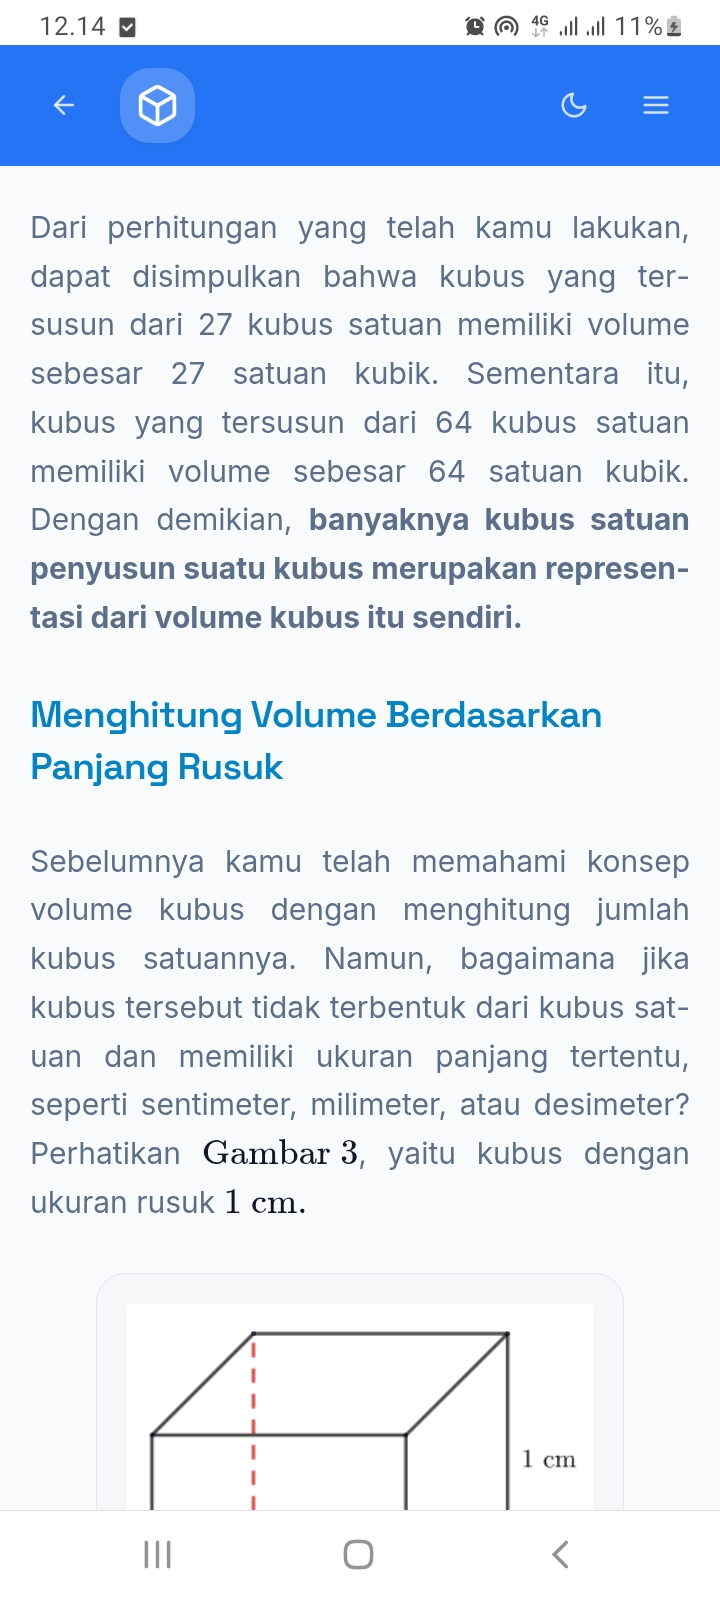
\includegraphics[width=0.25\textwidth]{revisi/sebelum/sebelumC.jpg} &
                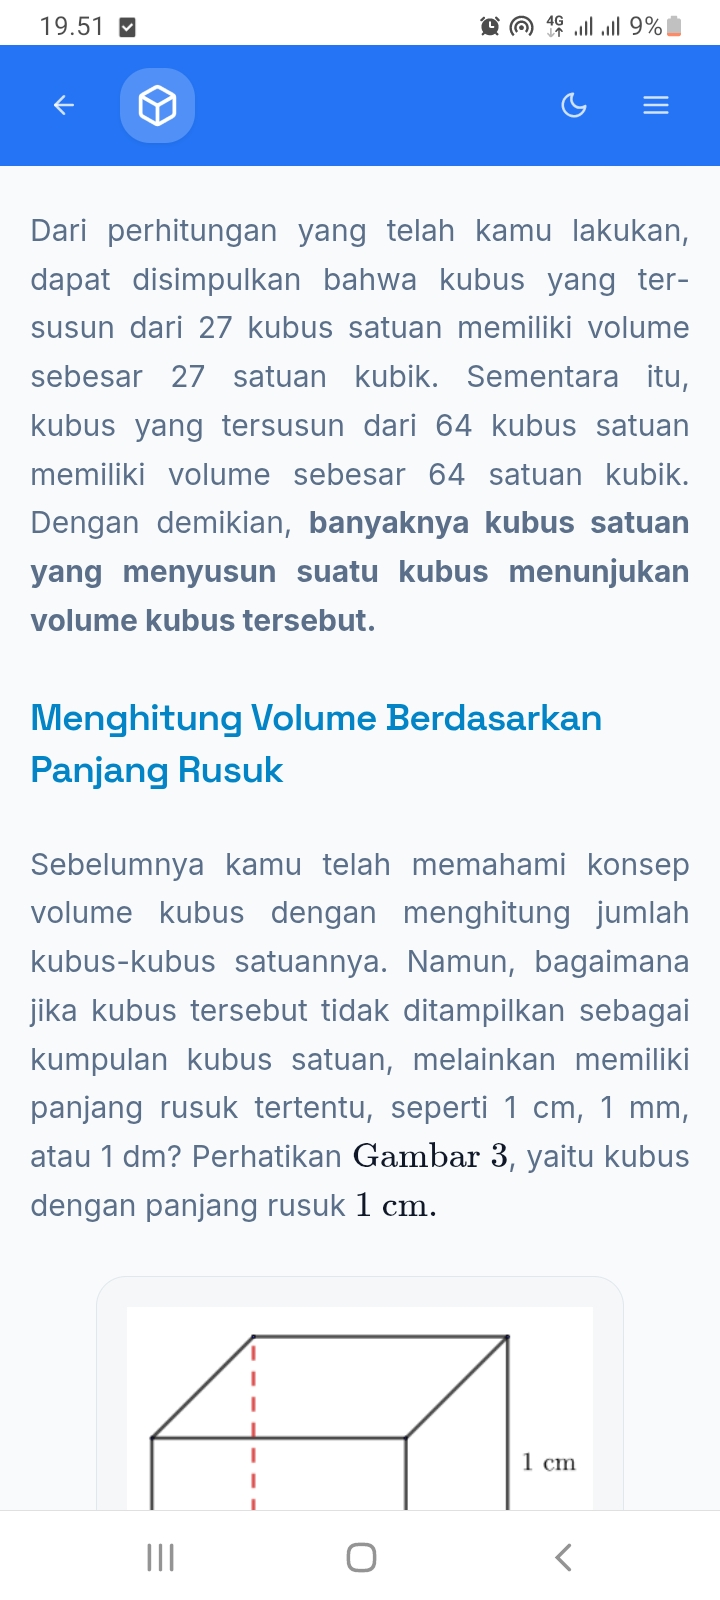
\includegraphics[width=0.25\textwidth]{revisi/sesudah/sesudahC.jpg} \\
            \end{tabular}
        \end{table}
        \item Memperbaiki definisi prisma agar tidak membingungkan siswa.
        \begin{table}[H]
            \centering
            \begin{tabular}{c c}
                Sebelum Revisi & Sesudah Revisi \\
                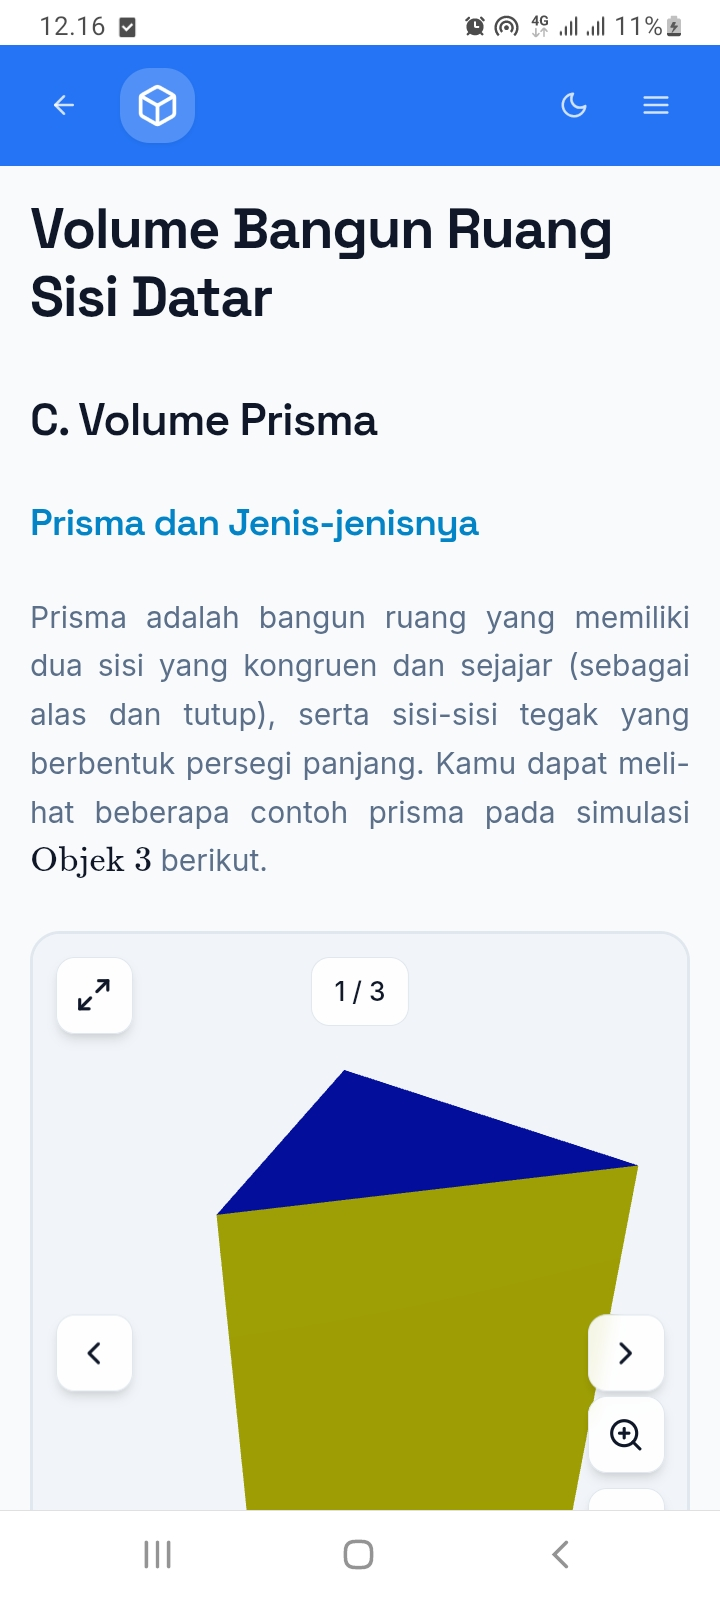
\includegraphics[width=0.25\textwidth]{revisi/sebelum/sebelumD.jpg} &
                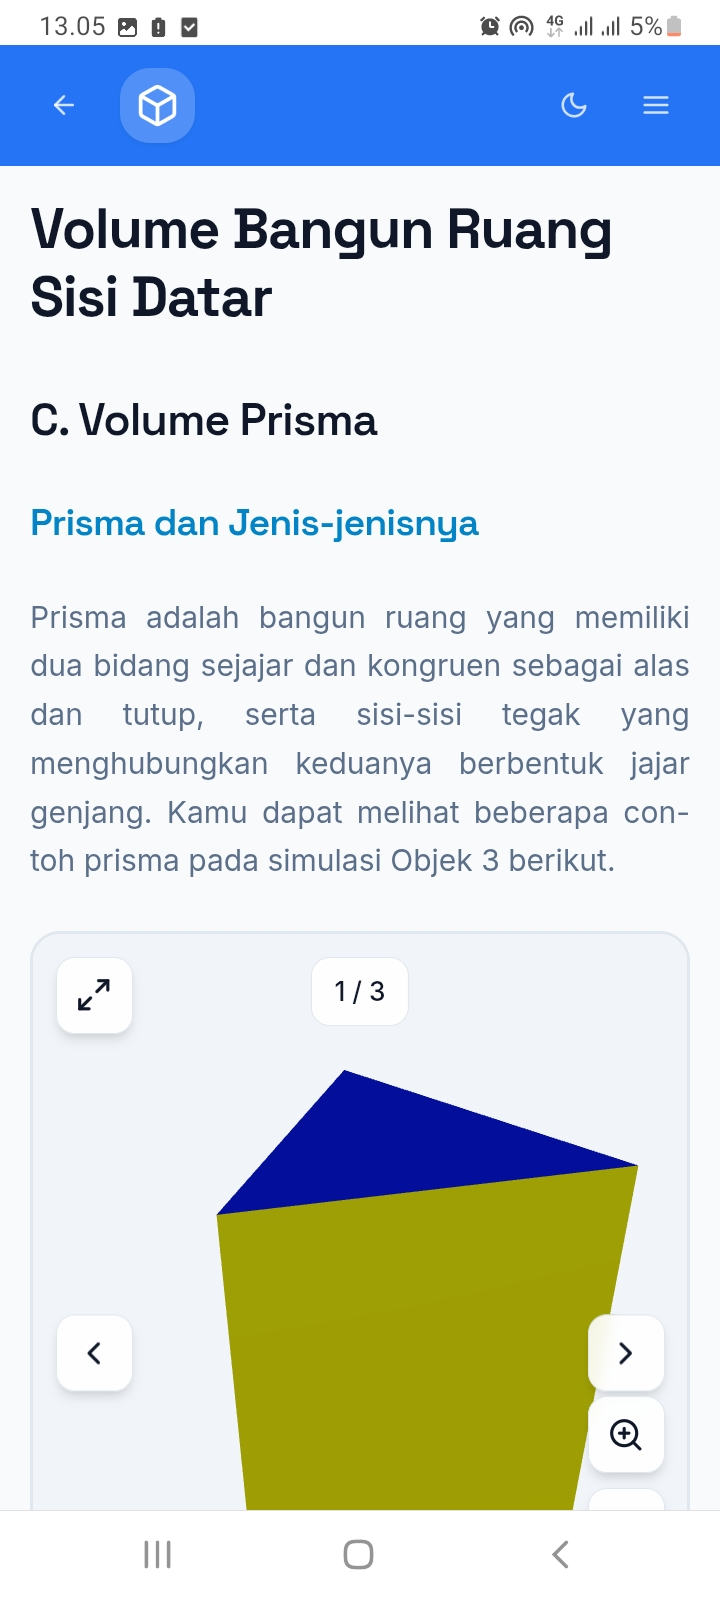
\includegraphics[width=0.25\textwidth]{revisi/sesudah/sesudahD.jpg} \\
            \end{tabular}
        \end{table}
        \item Menambahkan satu paragraf sebelum definisi jaring-jaring.
        \begin{table}[H]
            \centering
            \begin{tabular}{c c}
                Sebelum Revisi & Sesudah Revisi \\
                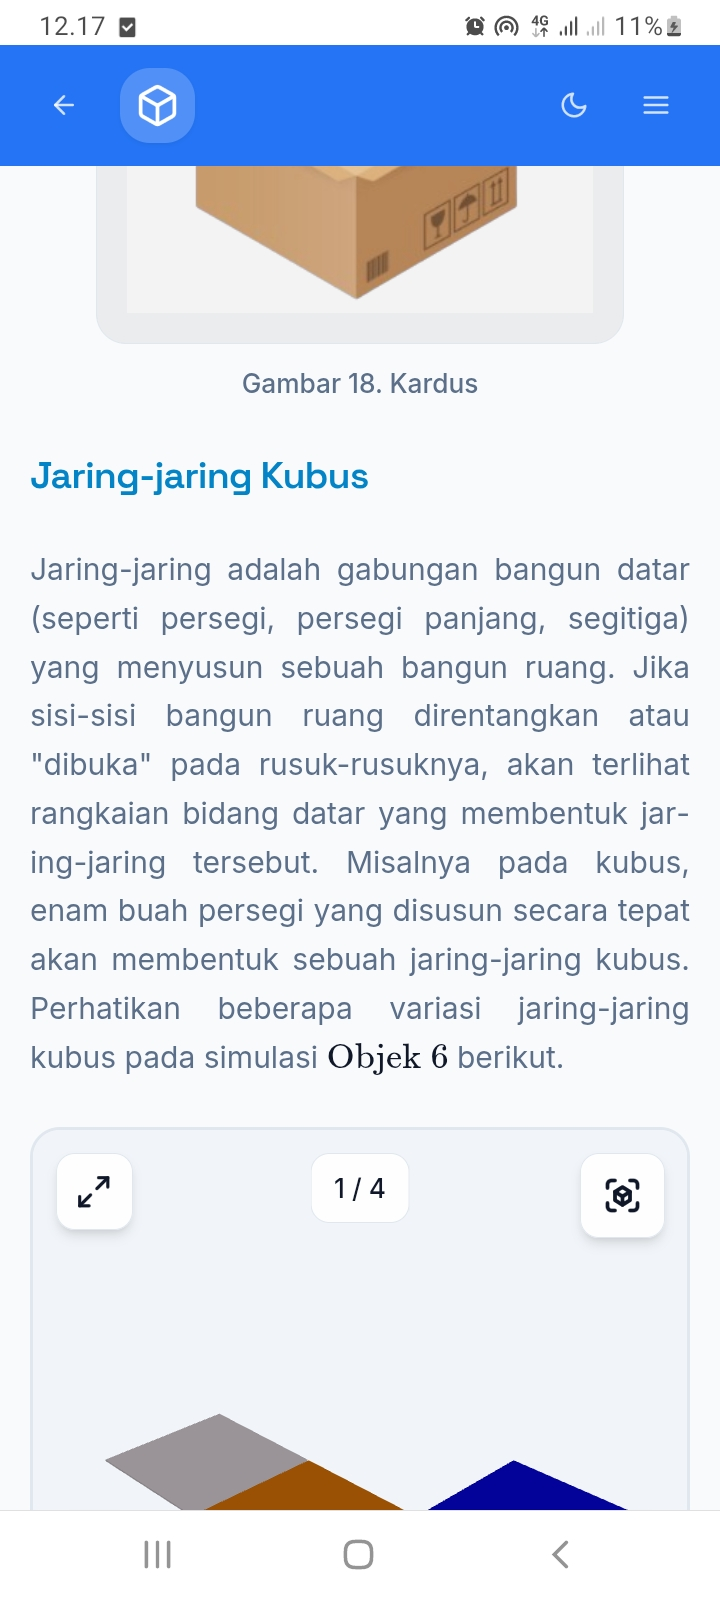
\includegraphics[width=0.25\textwidth]{revisi/sebelum/sebelumE.jpg} &
                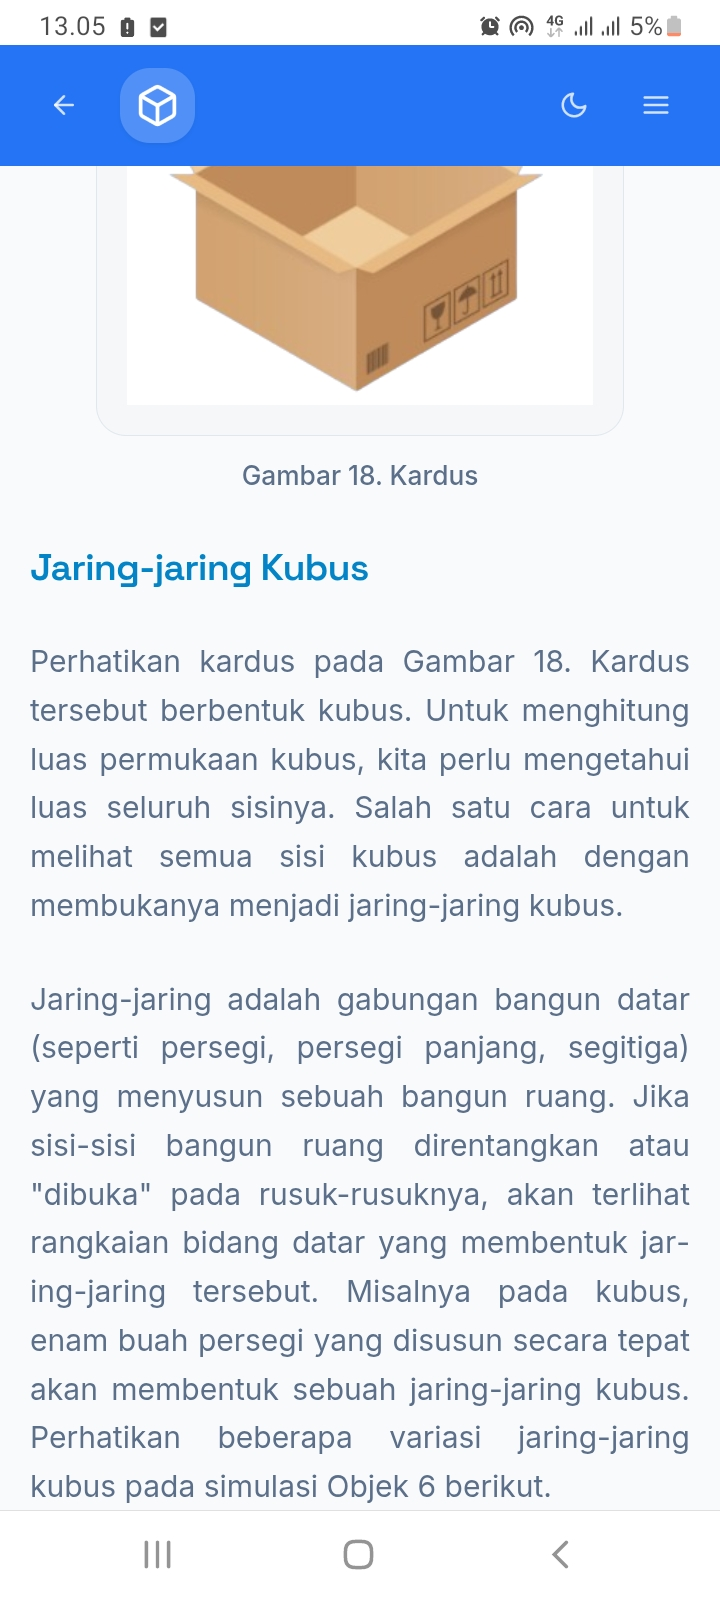
\includegraphics[width=0.25\textwidth]{revisi/sesudah/sesudahE.jpg} \\
            \end{tabular}
        \end{table}
        \item Menambah variasi jaring-jaring prisma.
        \begin{table}[H]
            \centering
            \begin{tabular}{c c}
                Sebelum Revisi & Sesudah Revisi \\
                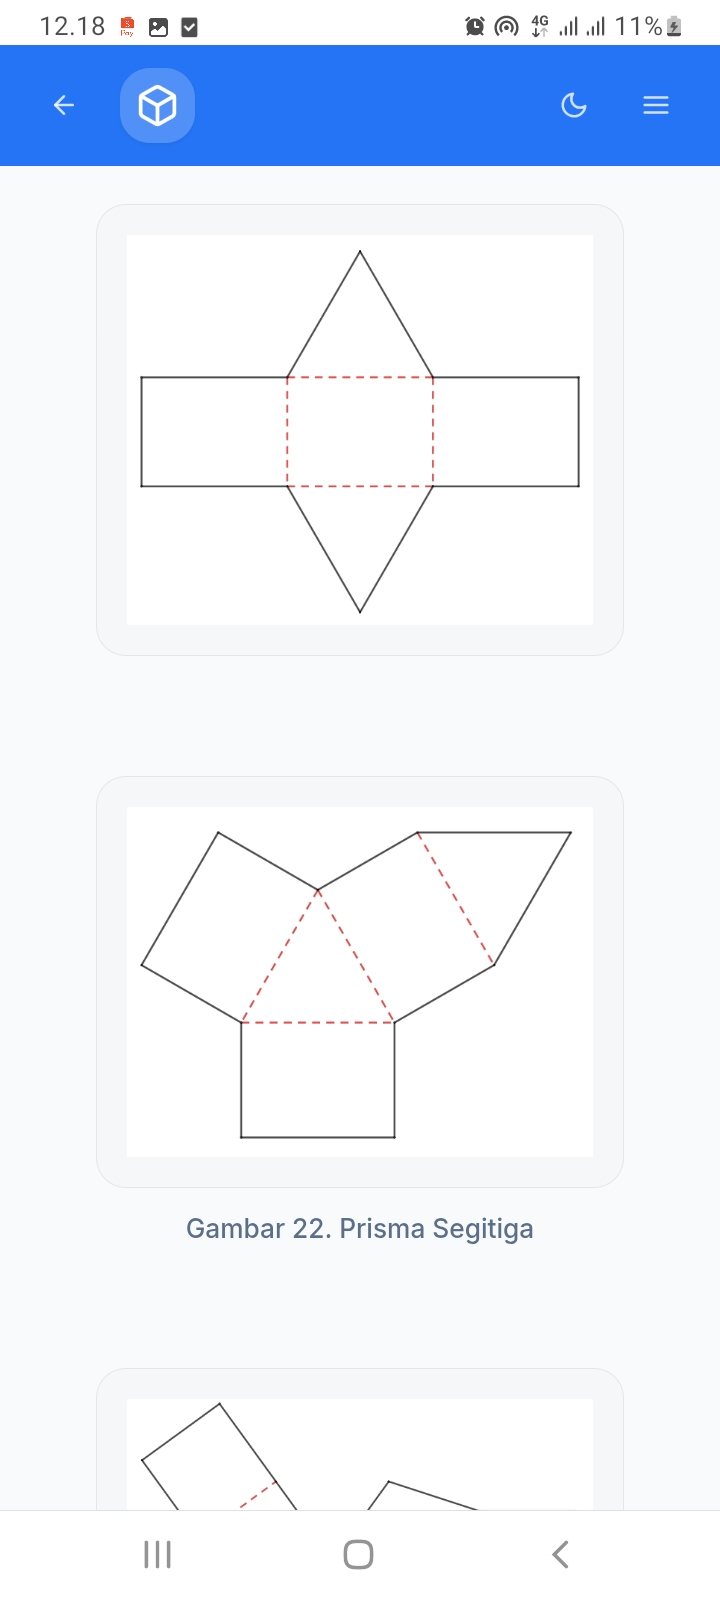
\includegraphics[width=0.25\textwidth]{revisi/sebelum/sebelumF.jpg} &
                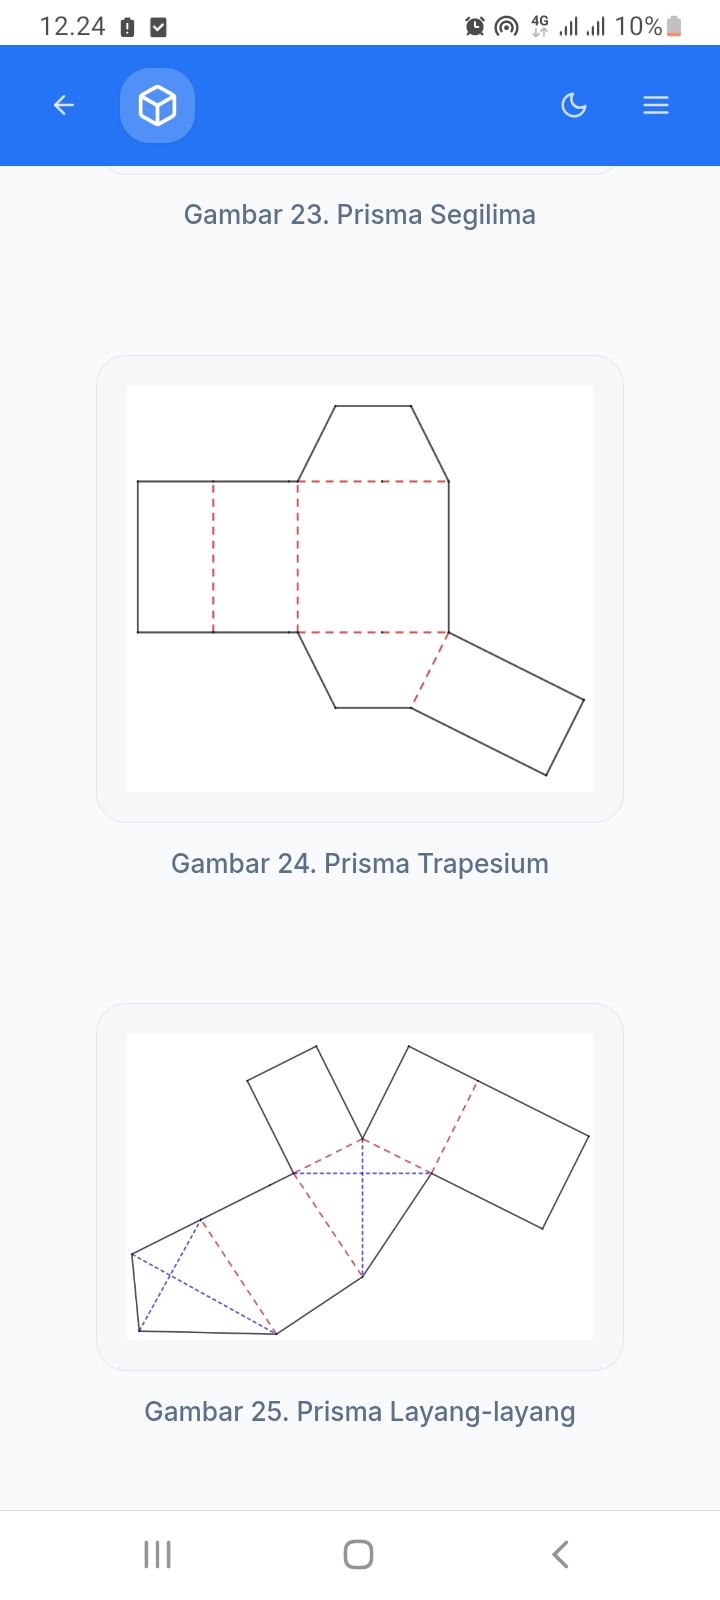
\includegraphics[width=0.25\textwidth]{revisi/sesudah/sesudahF.jpg} \\
            \end{tabular}
        \end{table}
        \item Menambahkan Capaian Pembelajaran, Indikator Pencapaian Kompetensi, dan Tujuan Pembelajaran.
        \begin{table}[H]
            \centering
            \begin{tabular}{c c c}
                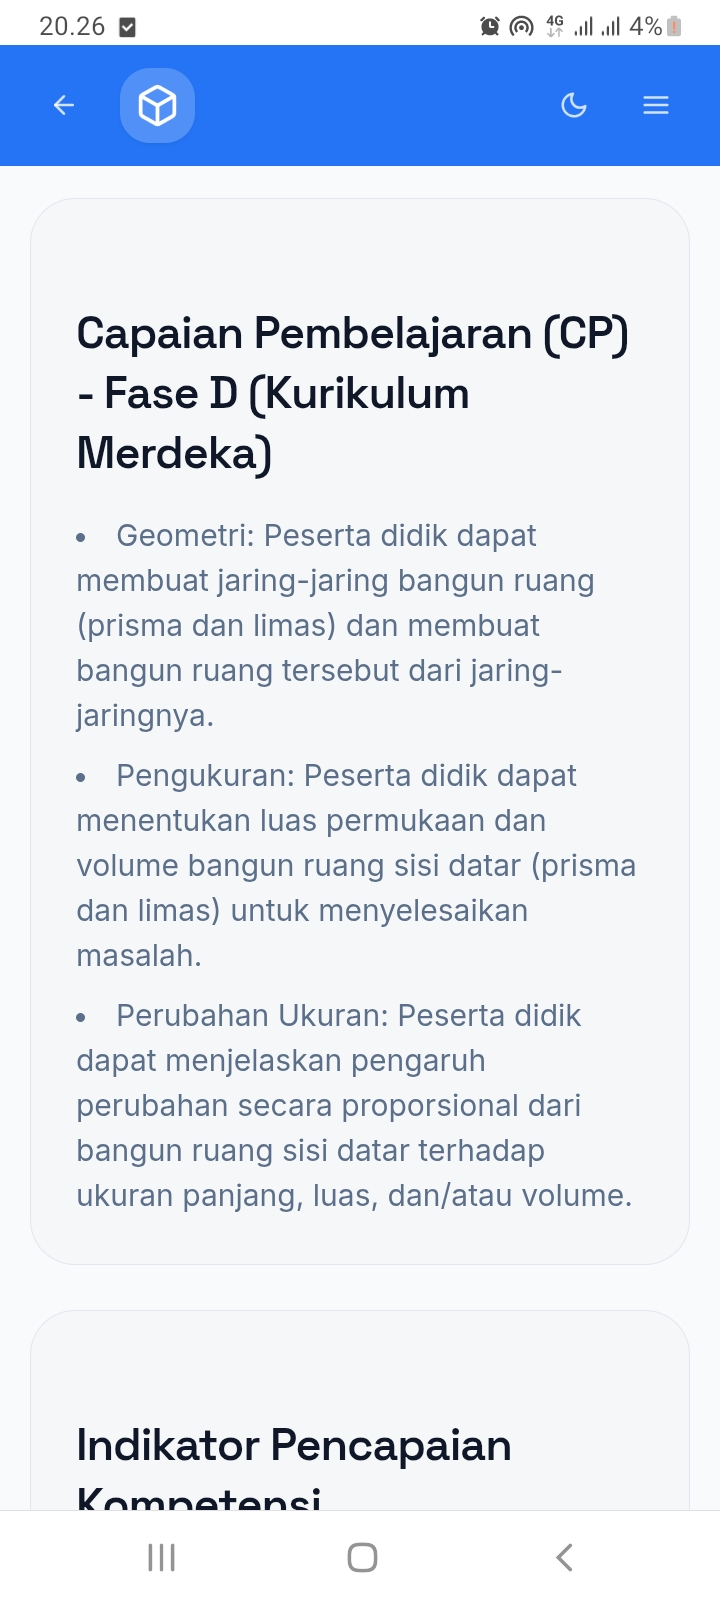
\includegraphics[width=0.25\textwidth]{revisi/sesudah/sesudahG1.jpg} &
                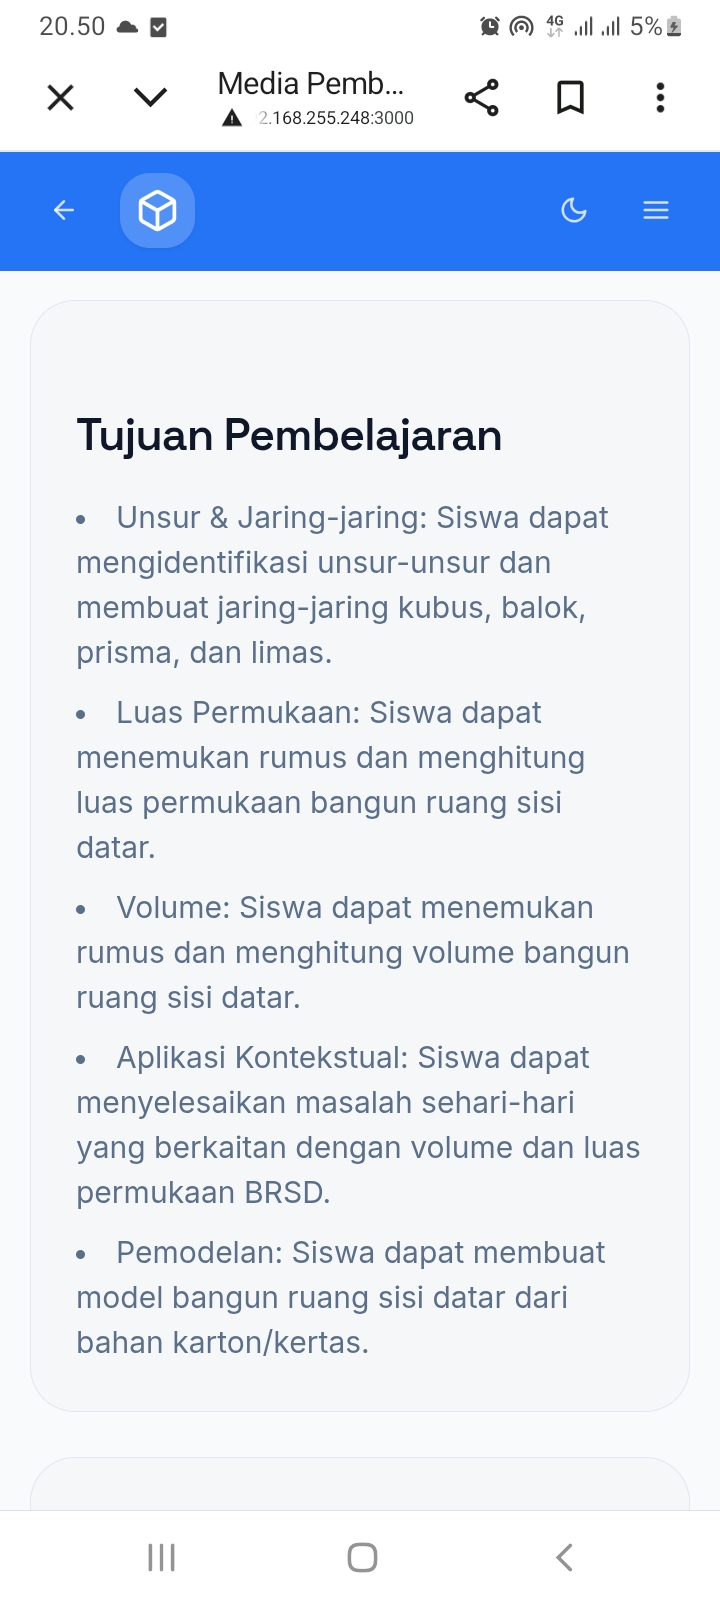
\includegraphics[width=0.25\textwidth]{revisi/sesudah/sesudahG2.jpg} &
                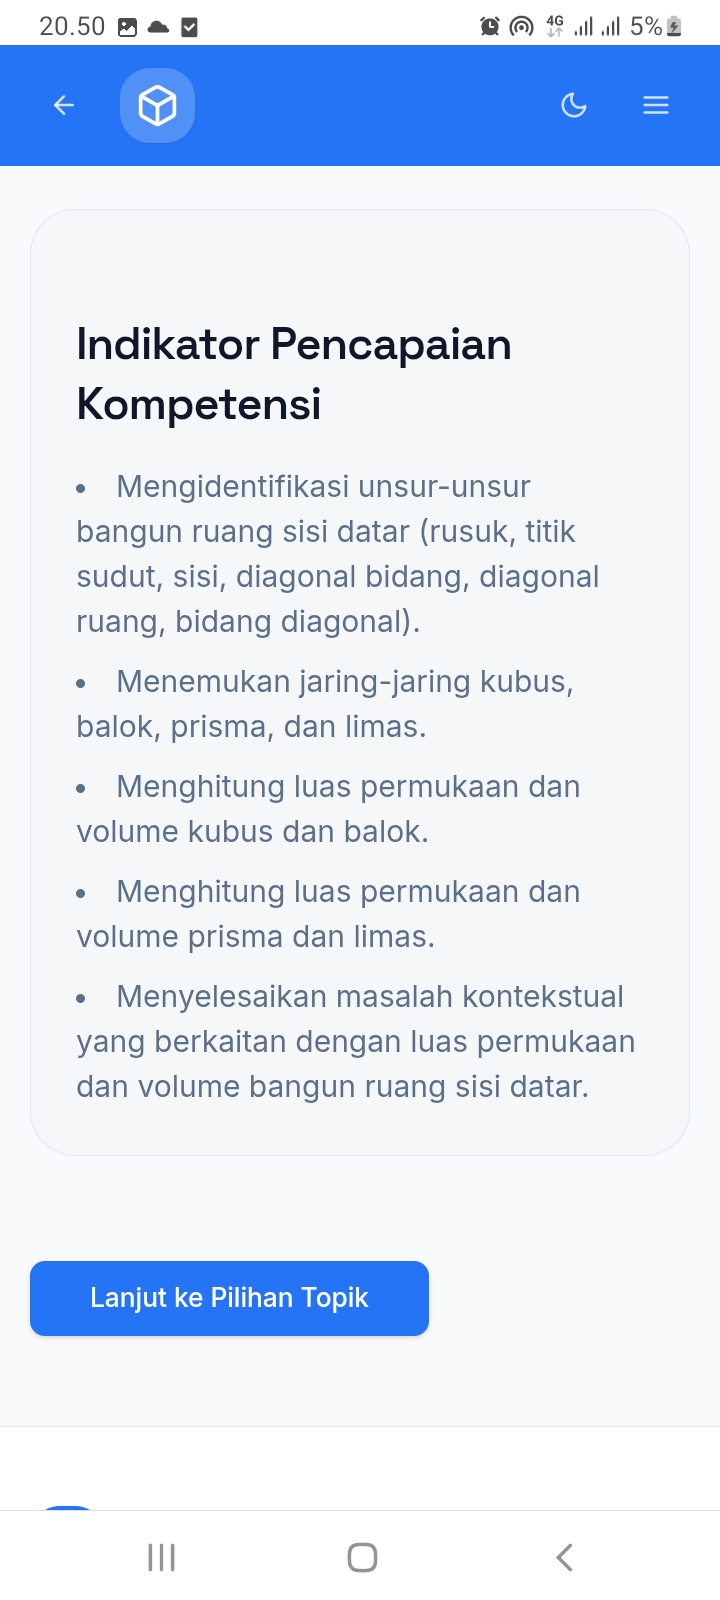
\includegraphics[width=0.25\textwidth]{revisi/sesudah/sesudahG3.jpg} \\
            \end{tabular}
        \end{table}
    \end{enumerate}
    \item Revisi Produk Hasil Validasi Ahli Media\\
    \hspace*{1cm}Revisi yang diberikan oleh ahli media tidak begitu banyak, hanya berfokus pada kunci jawaban banyak yang masih salah. Hasil perbaikan tersebut disajikan sebagai berikut.
    \begin{enumerate}
        \item Memperbaiki kunci jawaban.

         \begin{figure}[H]
            \centering
            \begin{tabular}{c c c}
                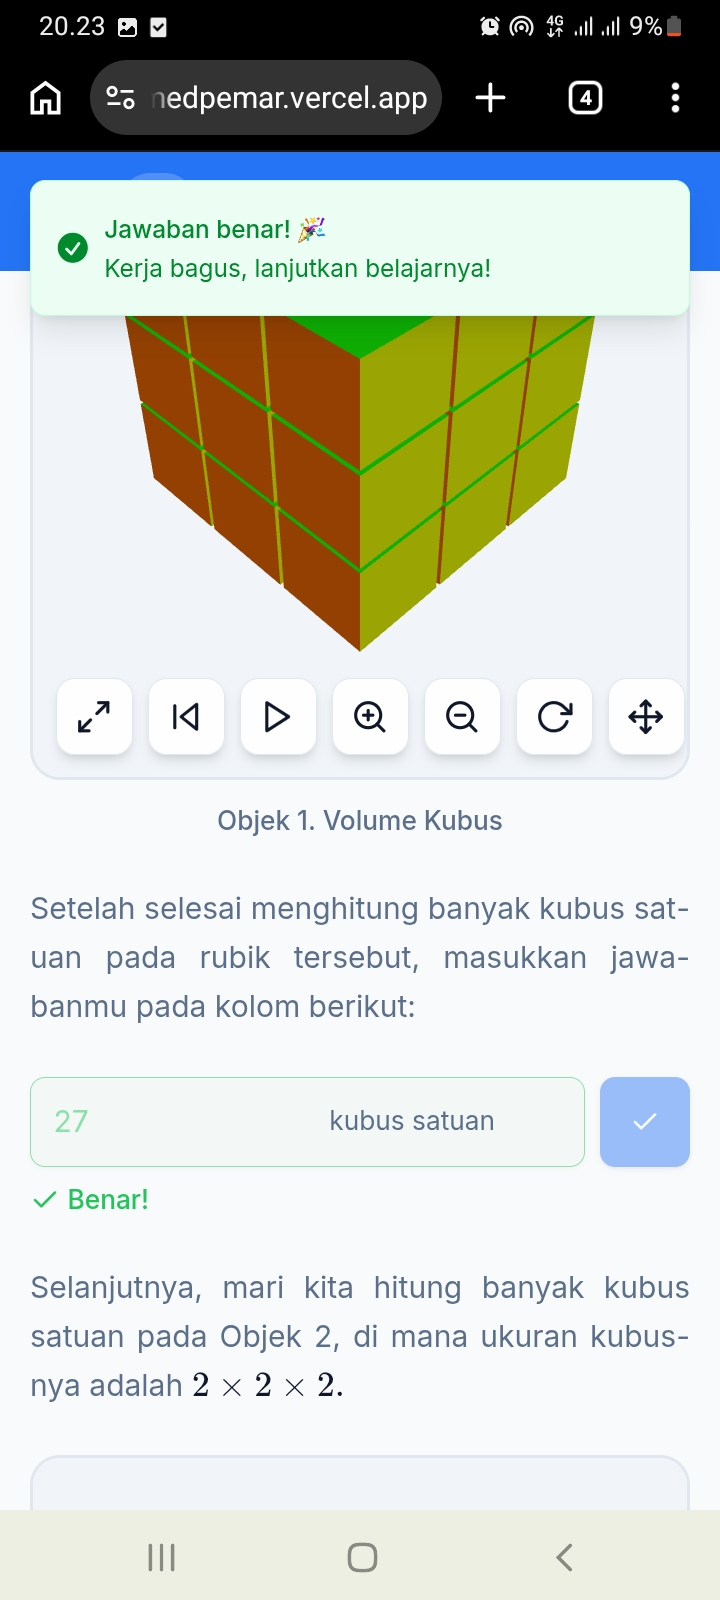
\includegraphics[width=0.25\textwidth]{revisi/Revisimedia2.jpg} &
                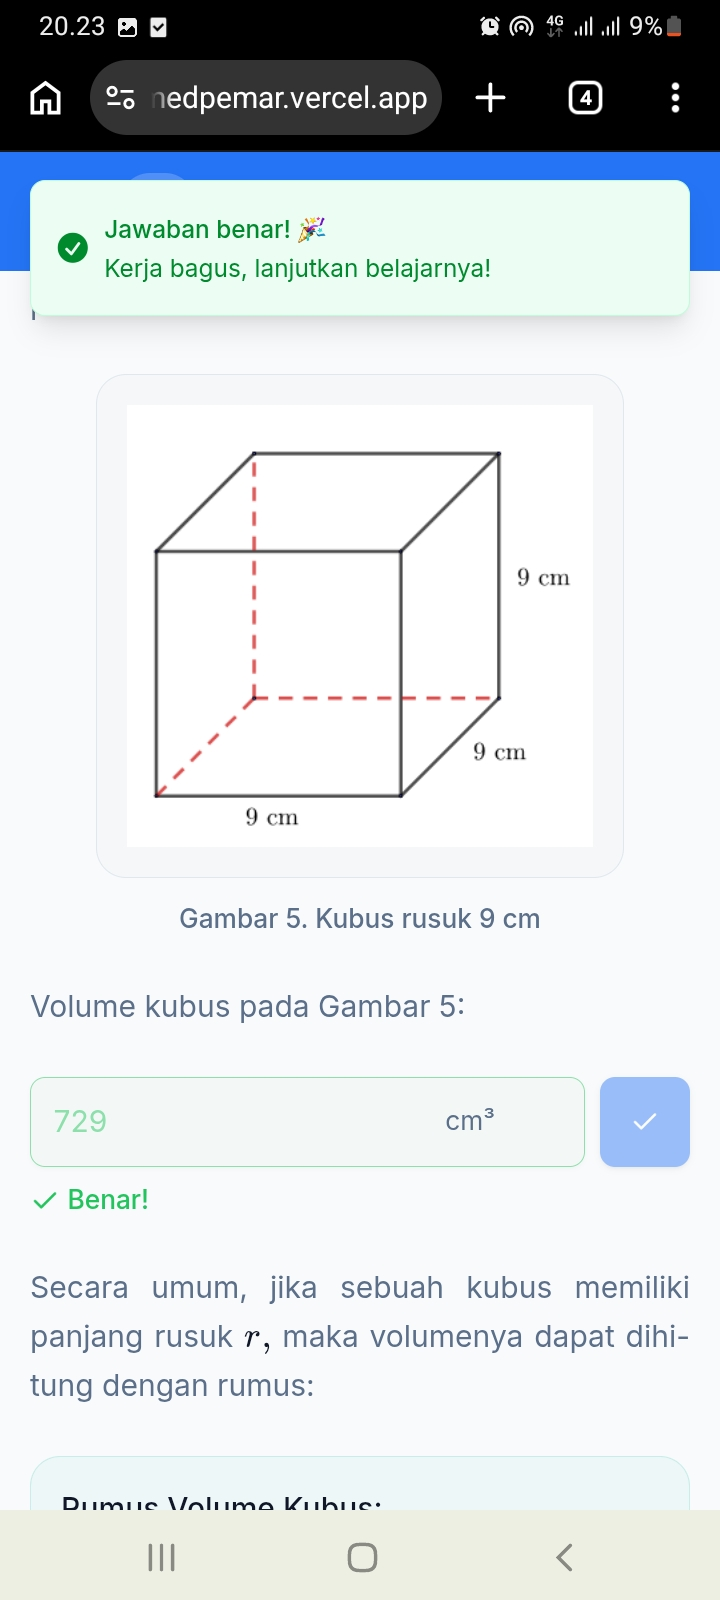
\includegraphics[width=0.25\textwidth]{revisi/Revisimedia.jpg} &
            \end{tabular}
                \caption{Contoh Perbaikan pada Kunci Jawaban}

        \end{figure}

    \end{enumerate}

    \item Revisi Produk Hasil Uji Coba Kelas Kecil\\
    \hspace*{1cm}Setelah melakukan ujicoba kelas kecil, tidak ada revisi yang disarankan oleh peserta didik.
\end{enumerate}

\textbf{D. Kajian Produk Akhir}
\addcontentsline{toc}{section}{D. Kajian Produk Akhir}

\hspace*{1cm}Media pembelajaran yang dikembangkan oleh peneliti disusun dengan isi sebagaimana sebuah website pada umumnya. Dimana media pembelajaran memiliki halaman awal \textit{(Landing Page)}, halaman menu, halaman petunjuk, halaman materi, dan halaman kuis. Beikut adalah penjelasan dan tampilan dari masing-masing halaman tersebut.
\begin{enumerate}
    \item Halaman Awal\\
    \hspace*{1cm}Halaman awal merupakan halaman pertama yang dikunjungi saat siswa mengakses tautan media pembelajaran di https://medpemar.vercel.app. Pada halaman ini siswa akan melihat judul media pembelajaran, penjelasan singkat terkait media, cakupan isi media, dan instansi pembuat media. Berikut tampilan halaman awal pada mode ponsel dan mode layar lebar/komputer.
    \begin{figure}[H]
            \centering
            \begin{tabular}{c c c}
                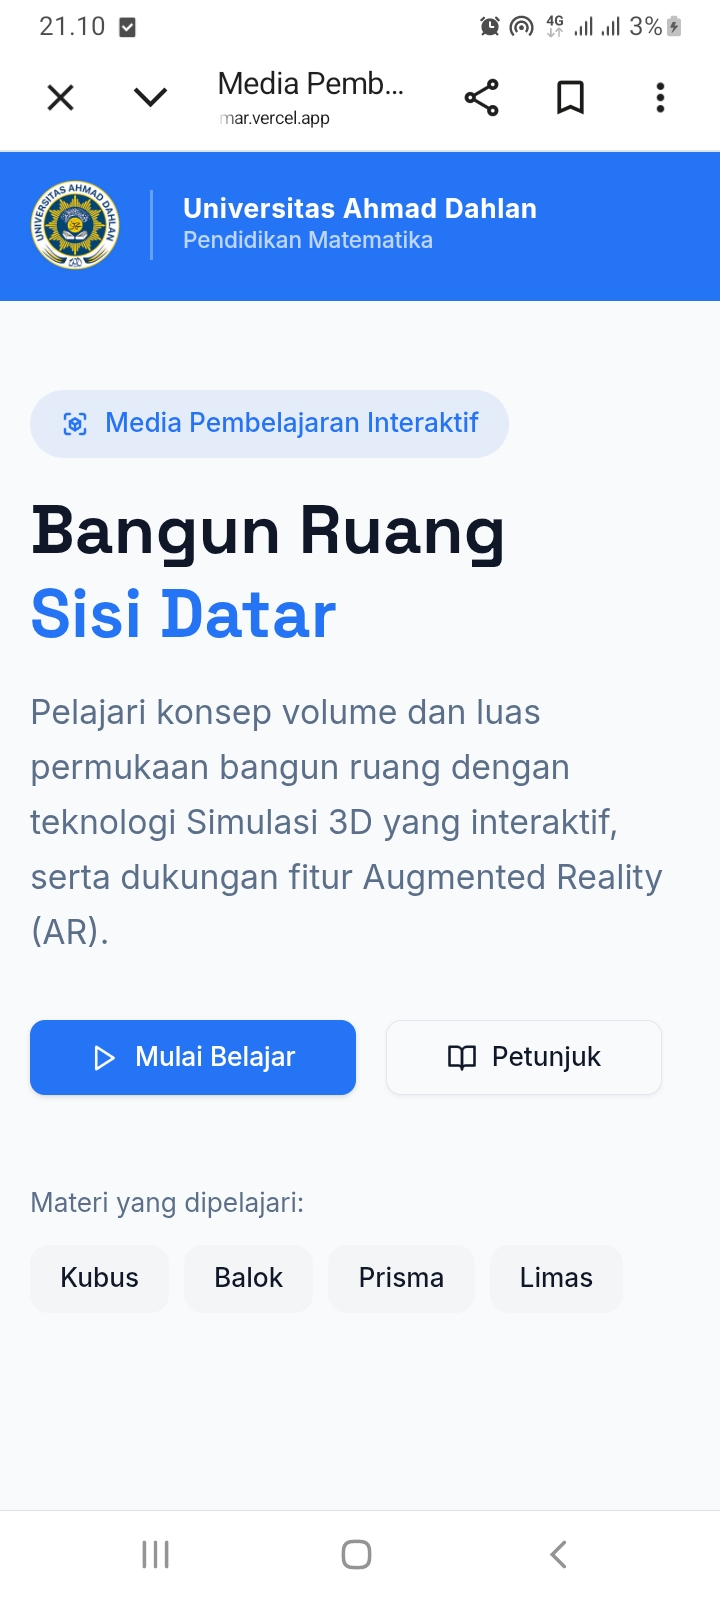
\includegraphics[width=0.25\textwidth]{revisi/Landingpage1.jpg} &
                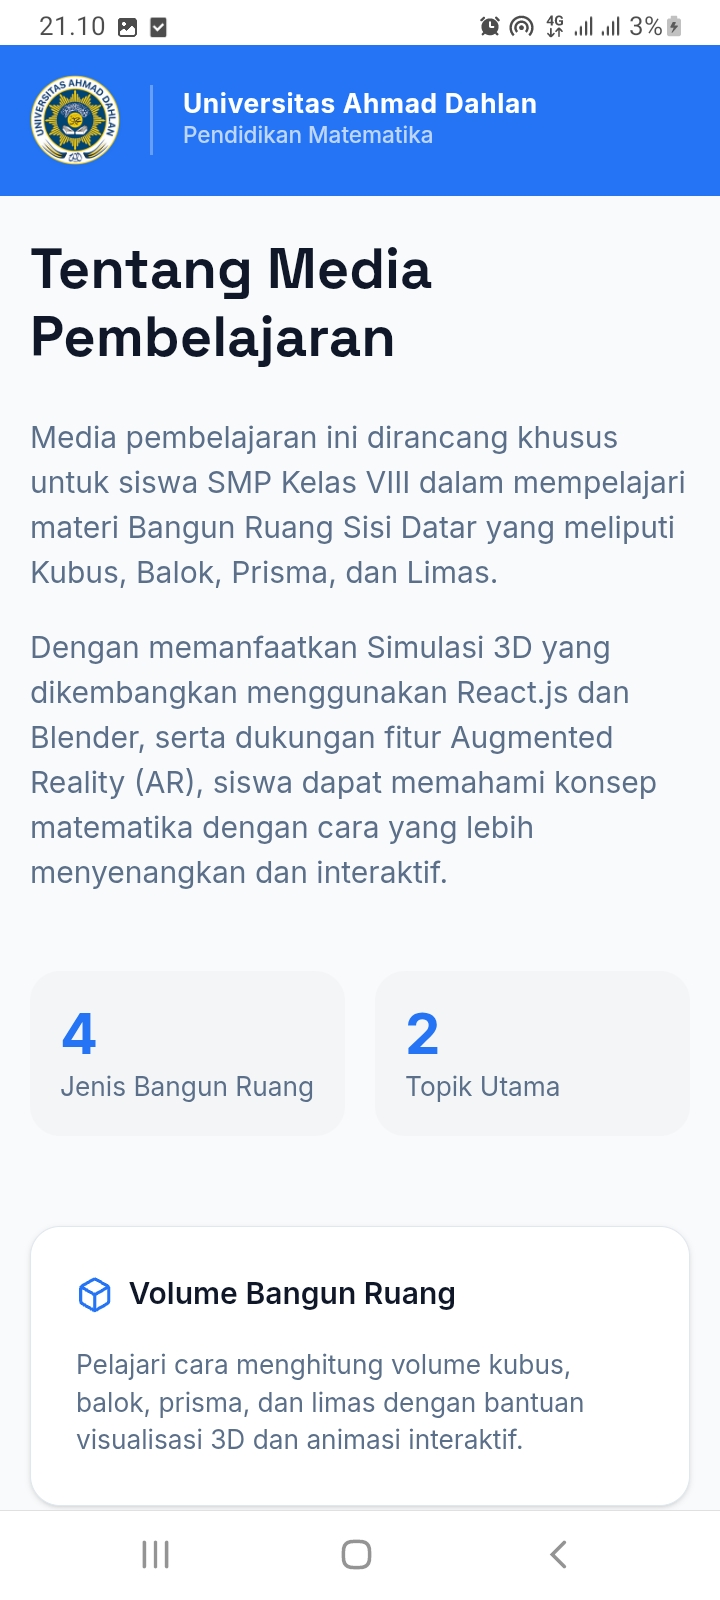
\includegraphics[width=0.25\textwidth]{revisi/Landingpage2.jpg} &
            \end{tabular}
                \caption{Landing Page versi Mobile}

        \end{figure}
        \begin{figure}[H]
            \centering
            \begin{tabular}{c c c}
                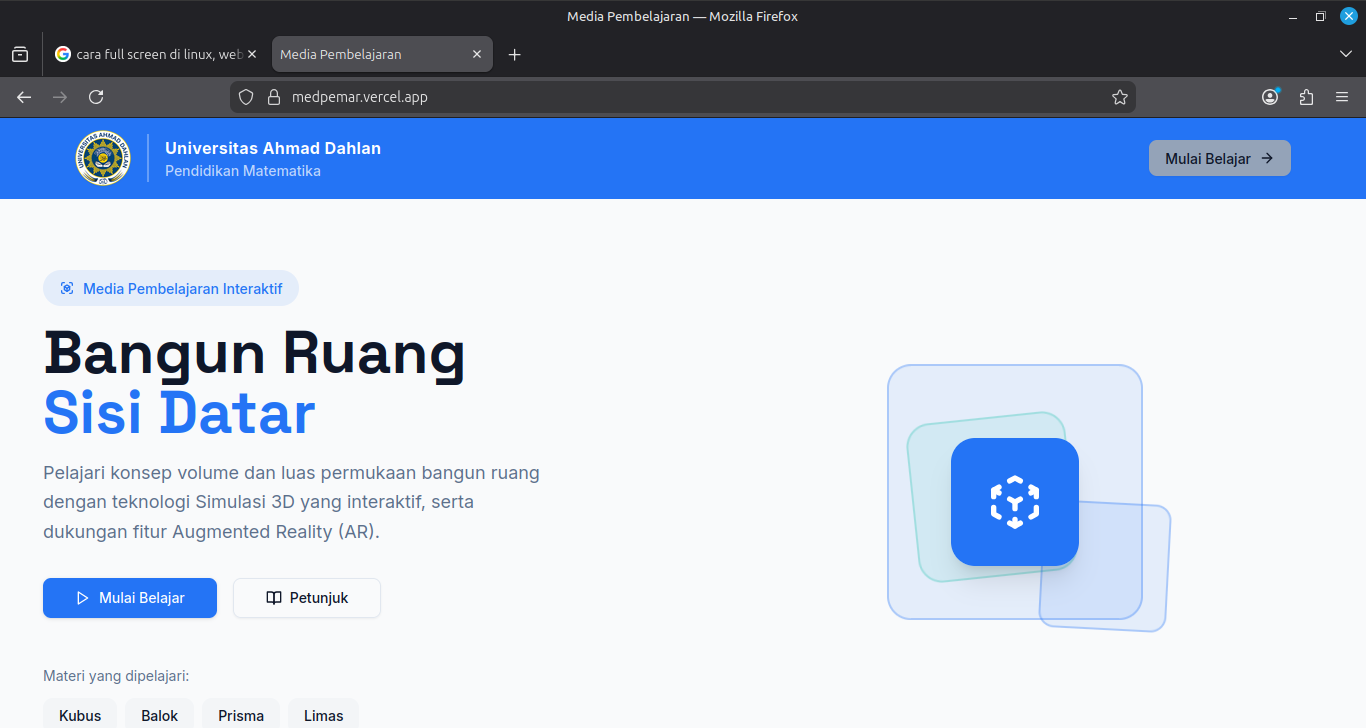
\includegraphics[width=1\textwidth]{revisi/Landingpage3.png} &
            \end{tabular}
                \caption{Landing Page versi Desktop}

        \end{figure}
    \item Halaman Pendahuluan Pembelajaran\\
    \hspace*{1cm}Halaman ini berisi tentang tujuan pembelajaran, capaian pembelajaran, dan indikator pencapaian kompetensi yang akan dipelajari oleh peserta didik.
    \begin{figure}[H]
            \centering
            \begin{tabular}{c c c}
                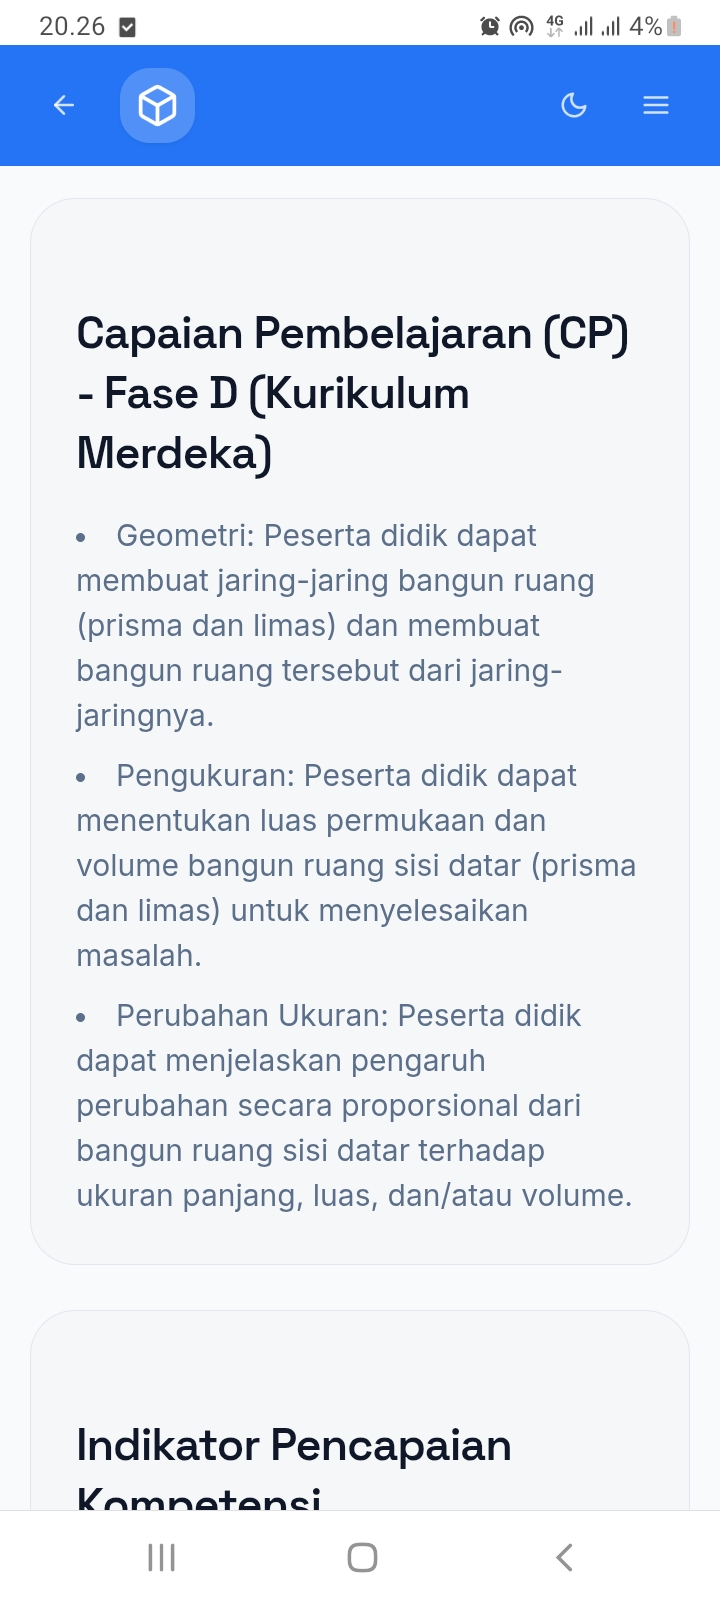
\includegraphics[width=0.3\textwidth]{revisi/sesudah/sesudahG1.jpg} &
                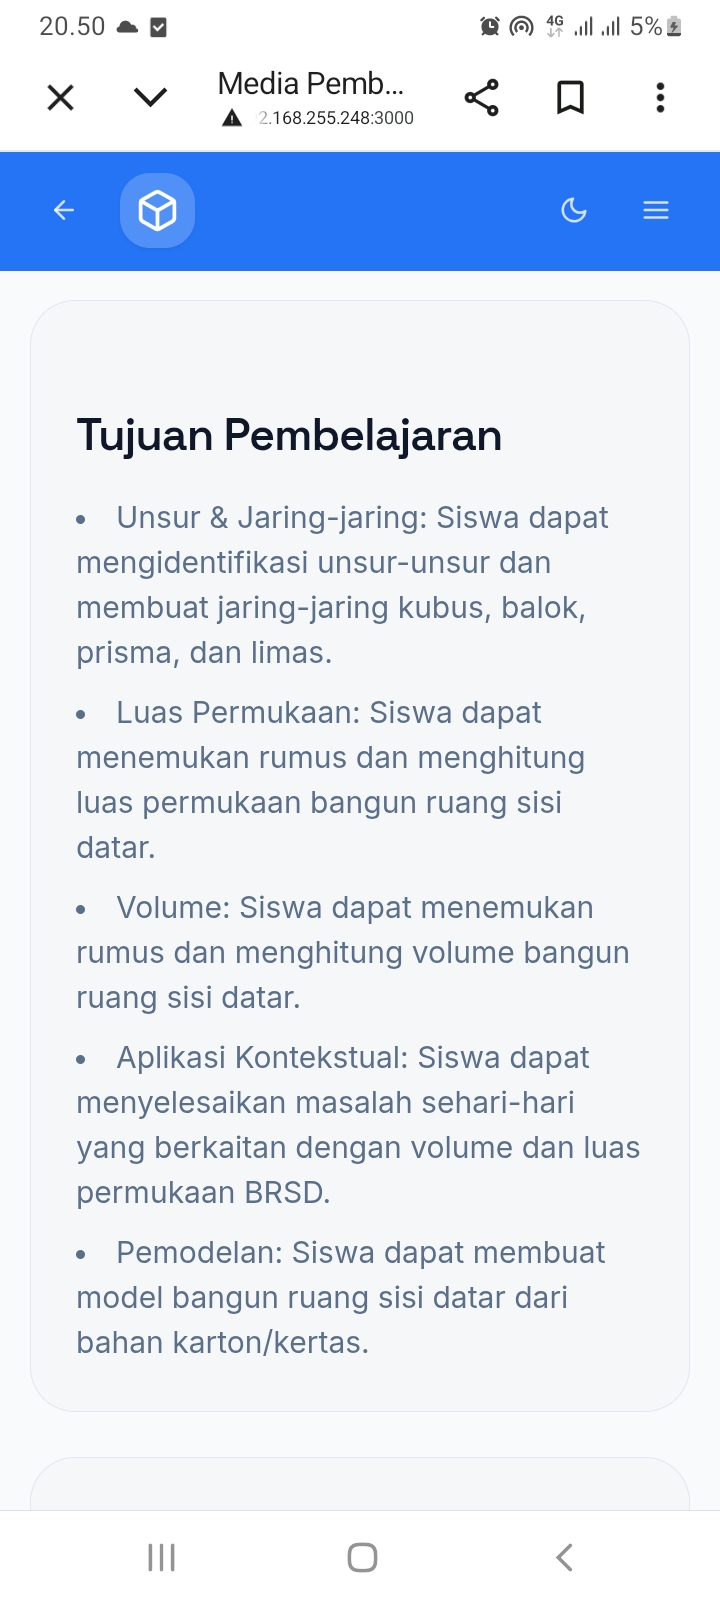
\includegraphics[width=0.3\textwidth]{revisi/sesudah/sesudahG2.jpg} &
                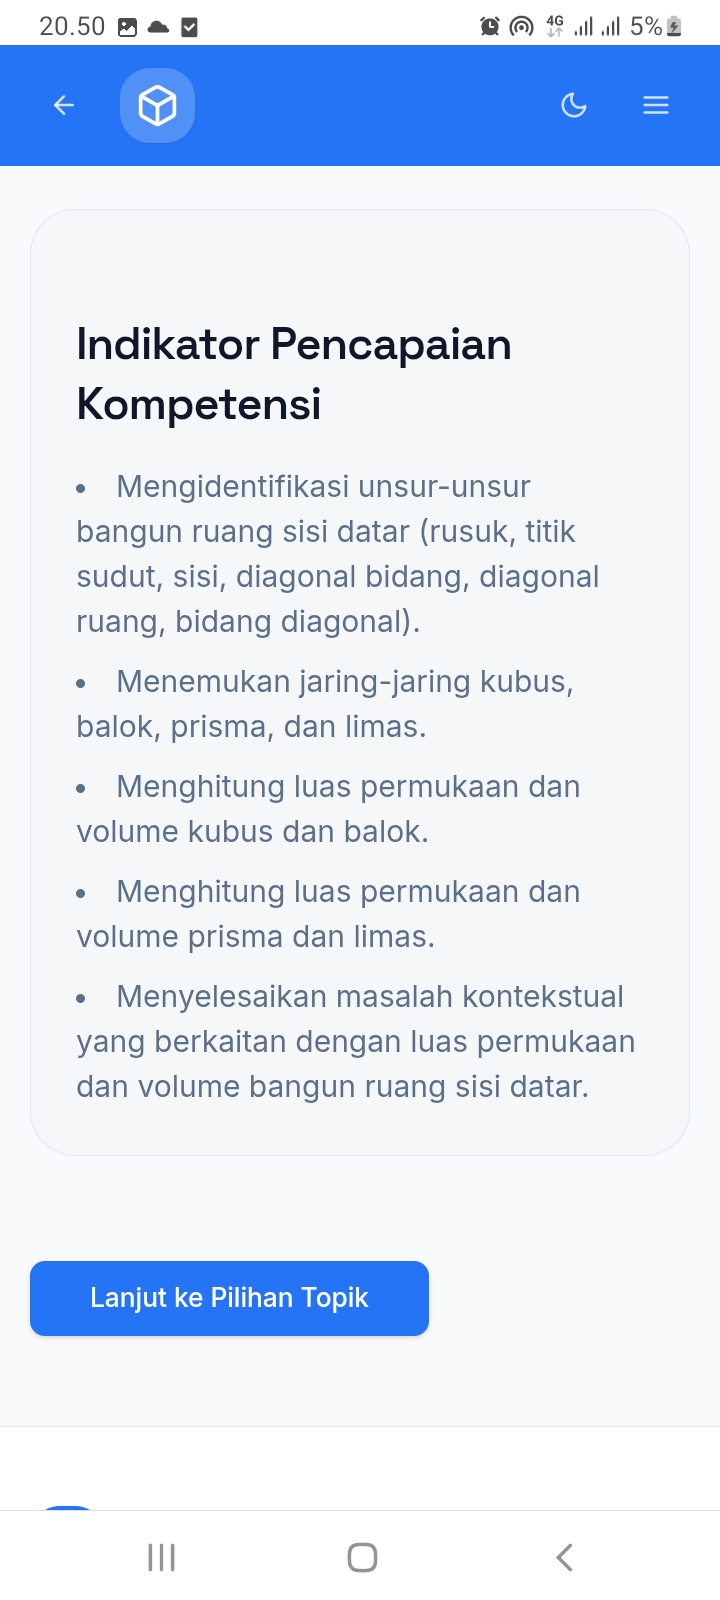
\includegraphics[width=0.3\textwidth]{revisi/sesudah/sesudahG3.jpg} \\
            \end{tabular}
                \caption{Halaman Pendahuluan Pembelajaran}

        \end{figure}
    \item Halaman Menu\\
    \hspace*{1cm}Pada halaman ini berisi pilihan materi yang akan dipelajari siswa, dan juga terdapat pilihan untuk ke halaman latihan soal. Pada halaman ini siswa juga bisa mengunduh barcode yang digunakan untuk menampilkan simulasi 3D.
    \begin{figure}[H]
            \centering
            \begin{tabular}{c c c}
                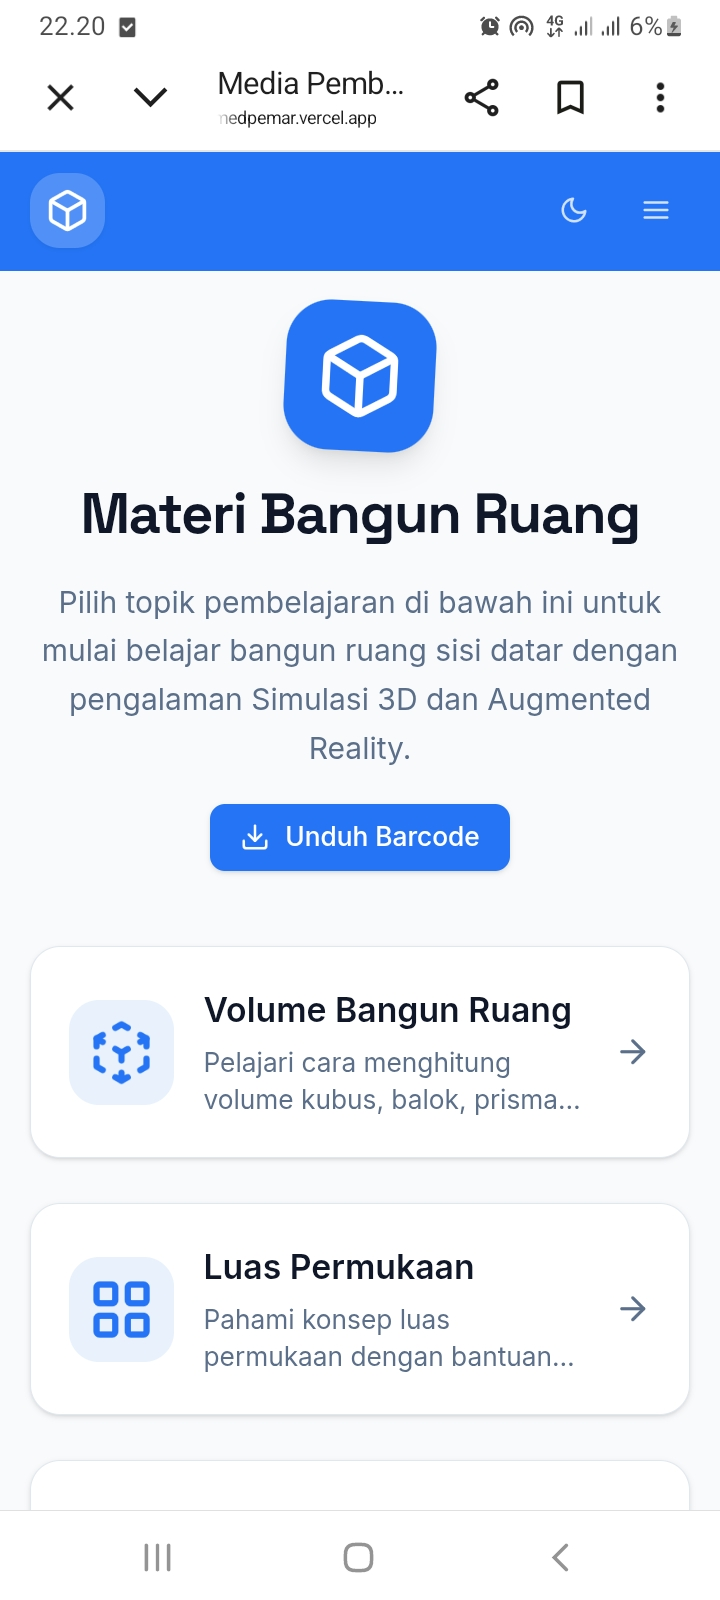
\includegraphics[width=0.3\textwidth]{revisi/Menu.jpg} &
                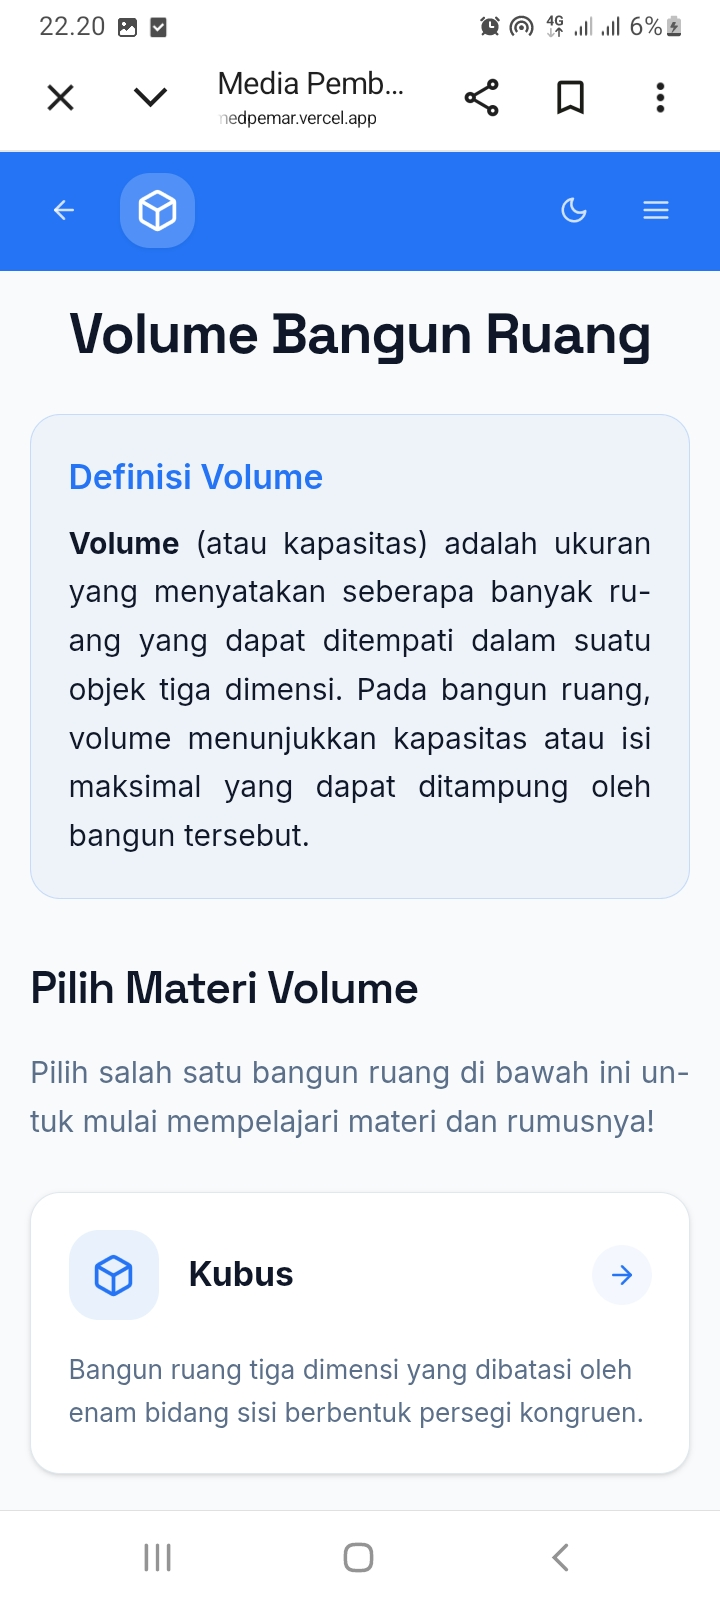
\includegraphics[width=0.3\textwidth]{revisi/Menuvolume.jpg} &
                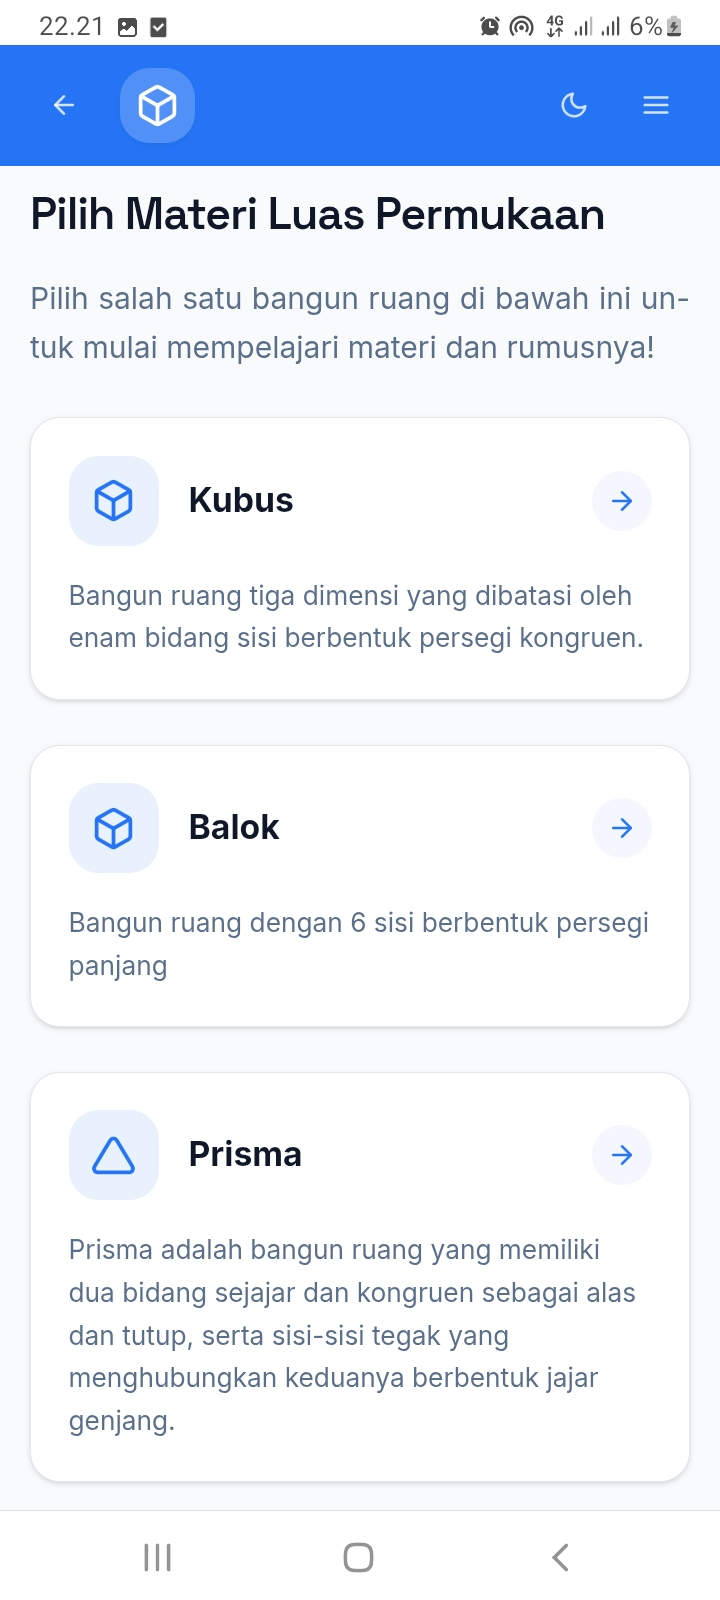
\includegraphics[width=0.3\textwidth]{revisi/Menuluaspermukaan.jpg} \\
            \end{tabular}
                \caption{Halaman Menu}

        \end{figure}

    \item Halaman Materi\\
    \hspace*{1cm}Pada halaman materi, peserta didik akan mempelajari dua topik utama, yaitu volume dan luas permukaan bangun ruang. Peserta didik akan melihat bangun ruang yang disajikan dalam bentuk 3D dan simulasi 3D. Bangun ruang tersebut juga dapat dianimasikan untuk mempermudah pemahaman. Untuk mengevaluasi pemahaman peserta didik, tersedia latihan soal dan pembahasan di akhir setiap bab.
    \begin{figure}[H]
        \centering
        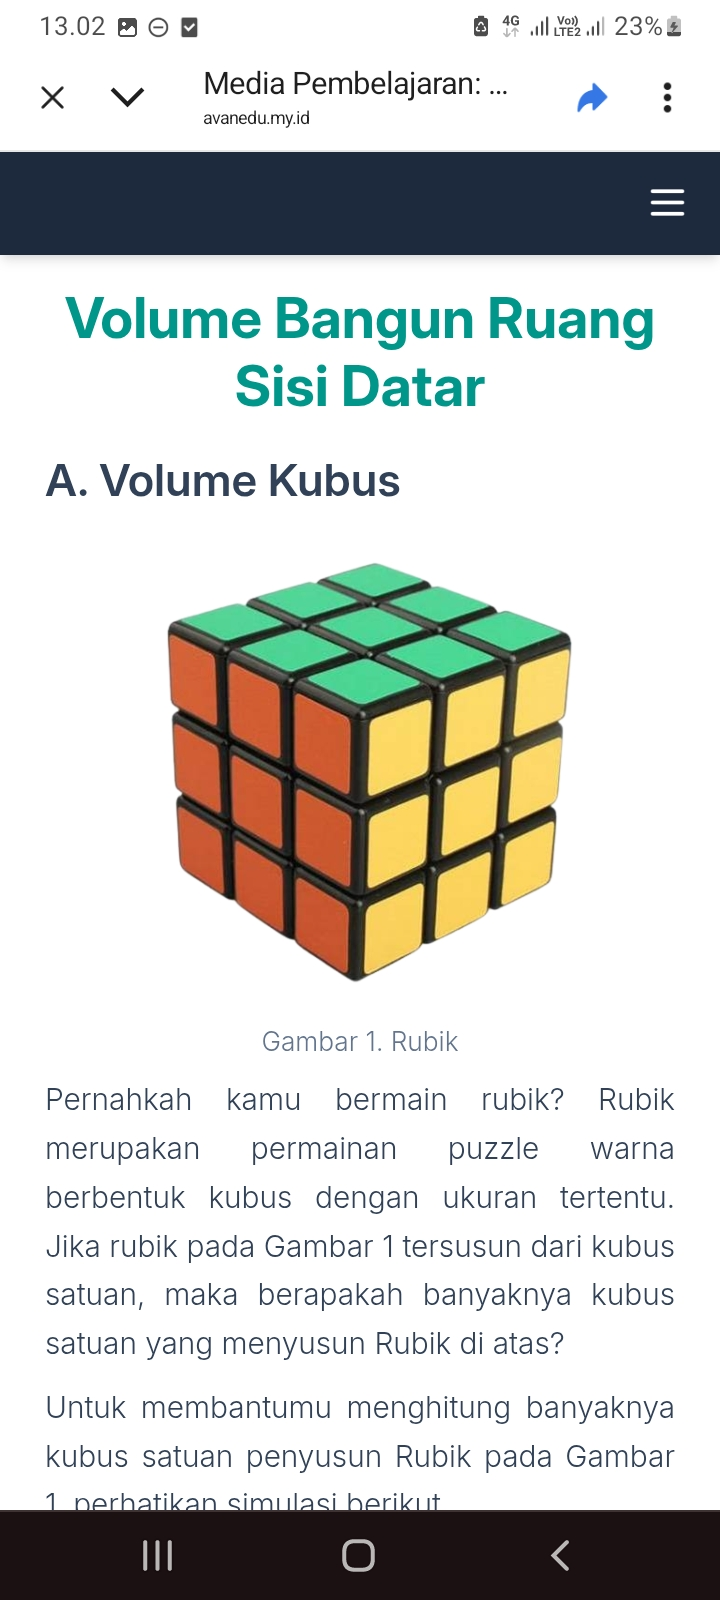
\includegraphics[width=0.2\textwidth]{images/materi1.jpg}
        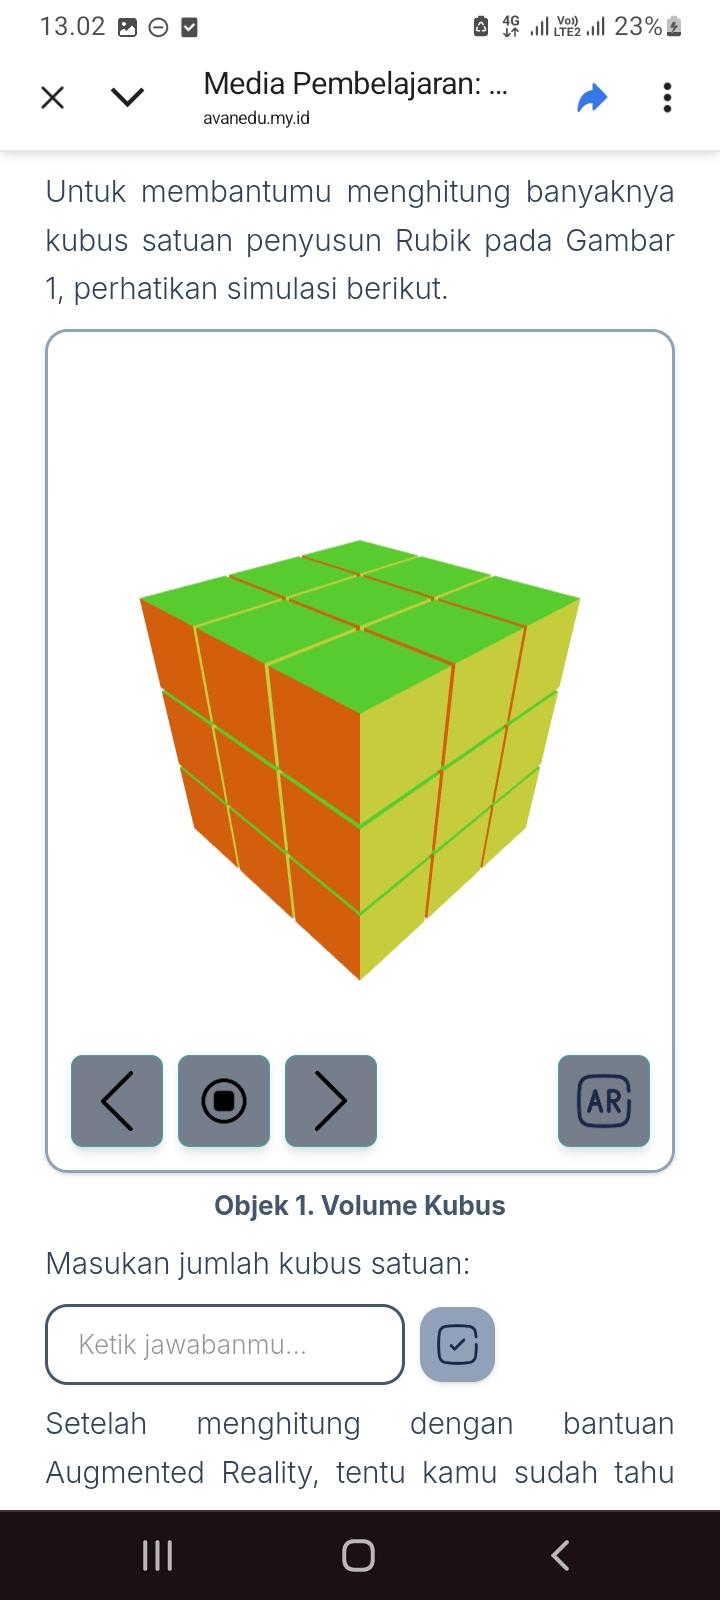
\includegraphics[width=0.2\textwidth]{images/materi2.jpg}
        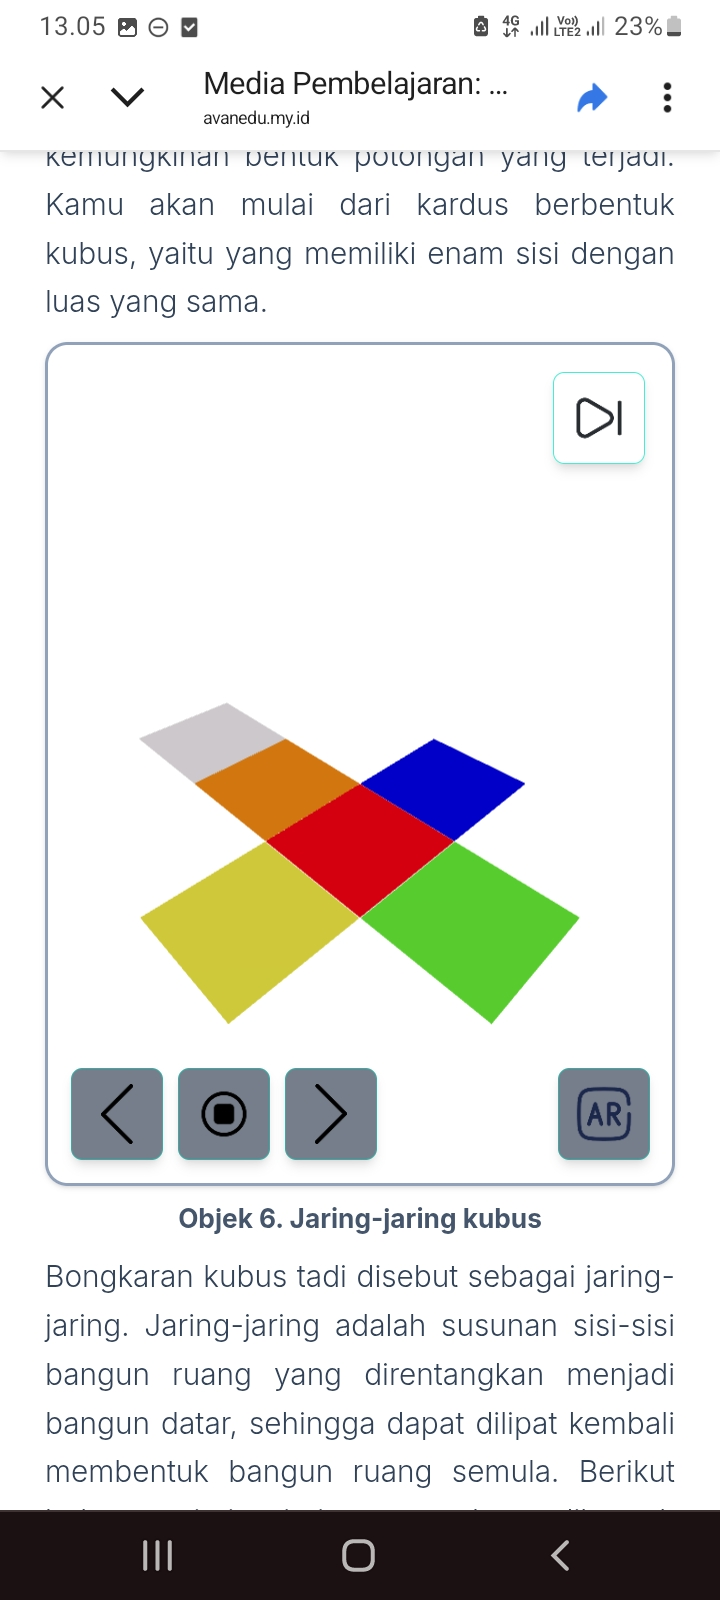
\includegraphics[width=0.2\textwidth]{images/materi3.jpg}
        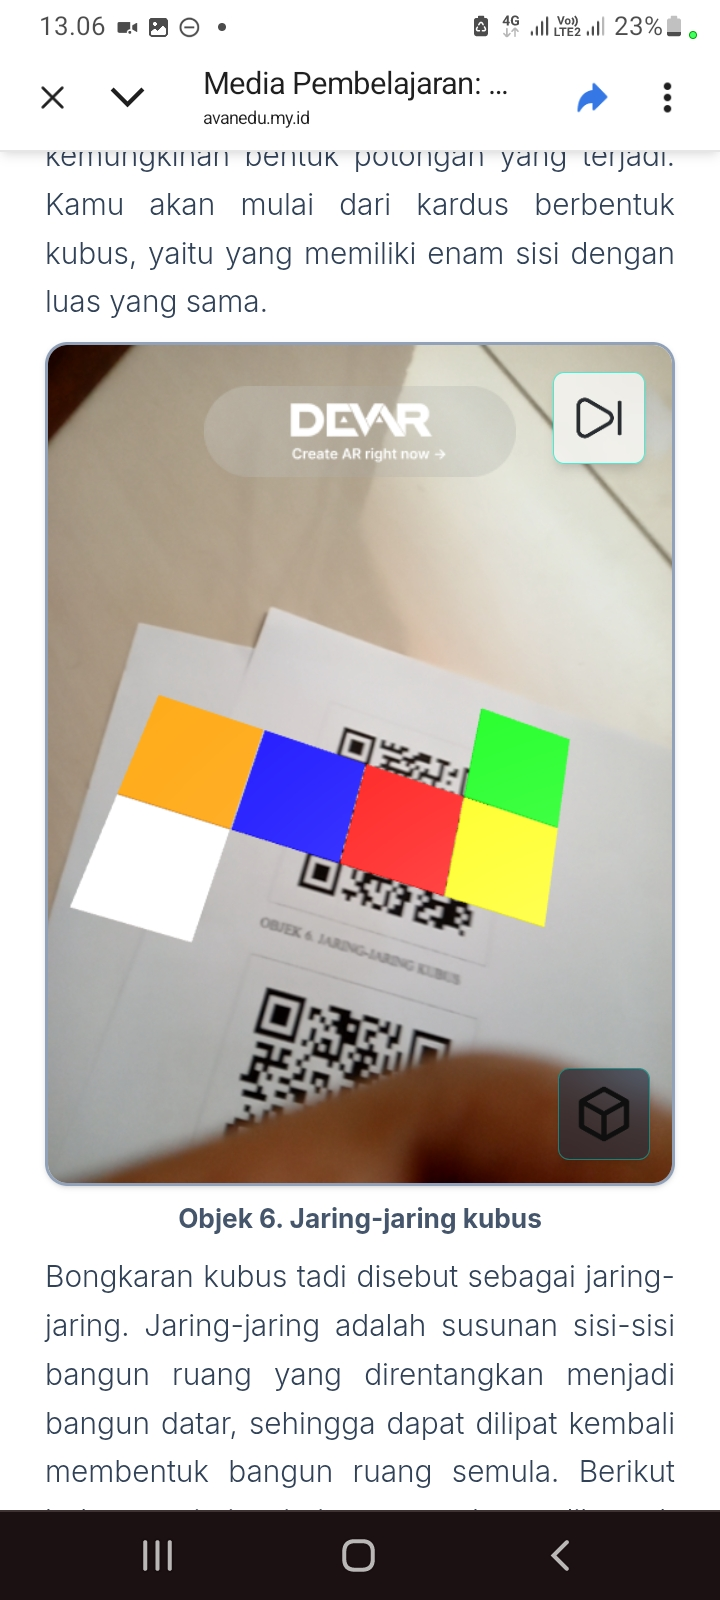
\includegraphics[width=0.2\textwidth]{images/materi4.jpg}
        \caption{Halaman Materi}
        \label{fig:materi}
    \end{figure}

    \item Halaman Kuis\\
    \hspace*{1cm}Pada halaman kuis, disajikan lima soal yang sesuai dengan latihan soal di akhir setiap bab. Terdapat juga penghitung waktu (timer) dengan batas waktu pengerjaan selama 30 menit. Untuk mulai mengerjakan kuis, peserta didik perlu memasukkan kode ujian. Peserta didik dapat menjawab soal dengan mengisi kolom jawaban yang disediakan, serta dapat menyisipkan foto untuk memperkuat jawabannya.
    \begin{figure}[H]
        \centering
        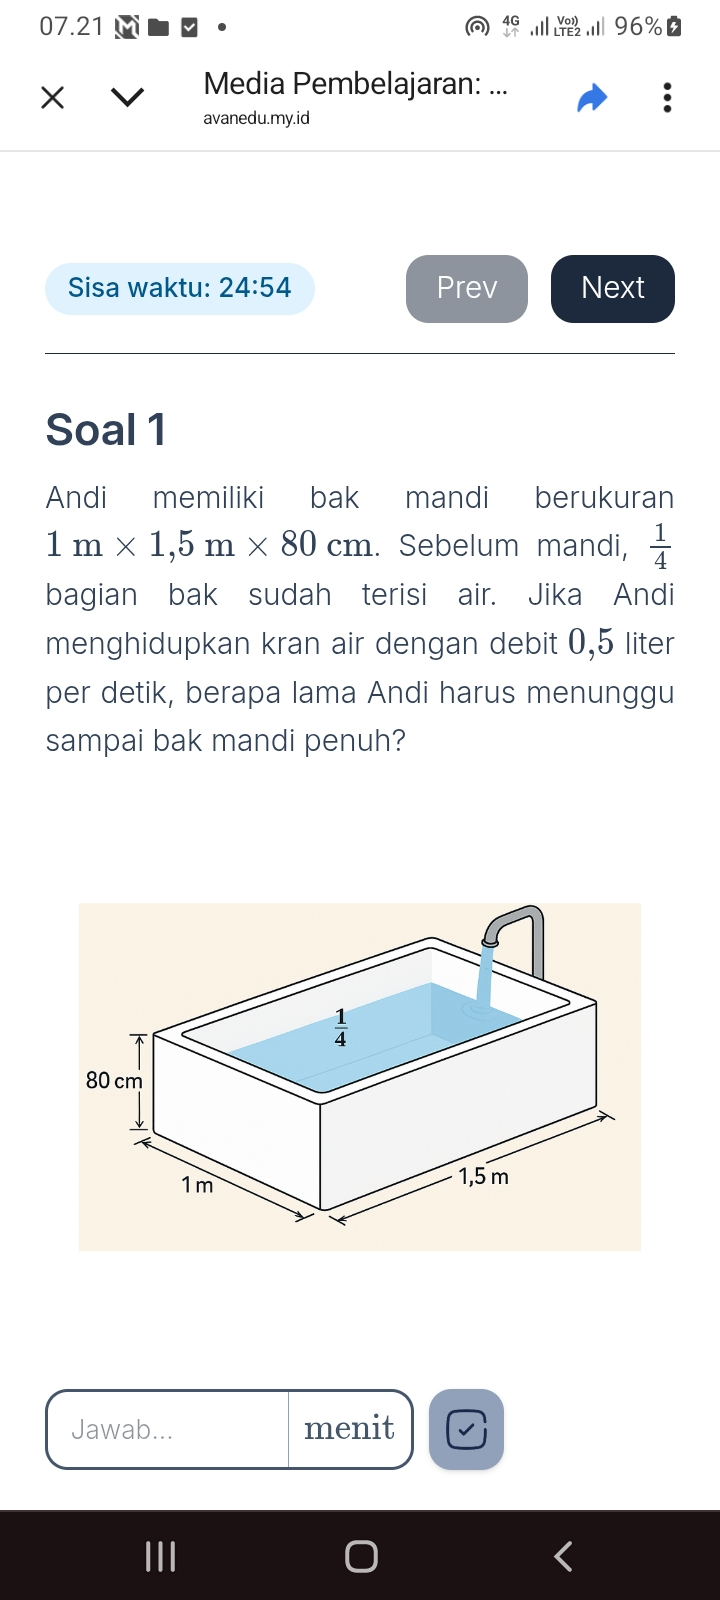
\includegraphics[width=0.25\textwidth]{images/kuis1.jpg}
        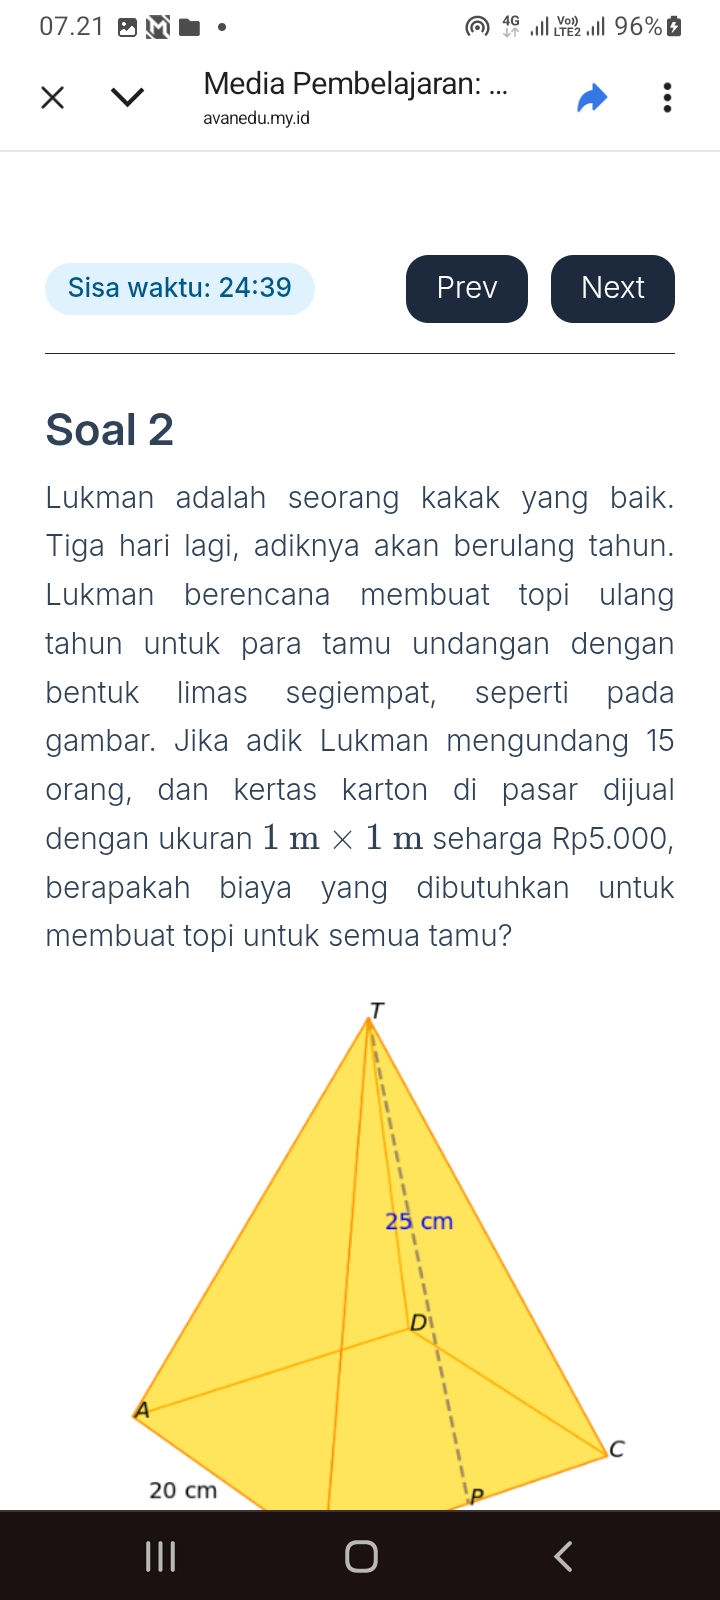
\includegraphics[width=0.25\textwidth]{images/kuis2.jpg}
        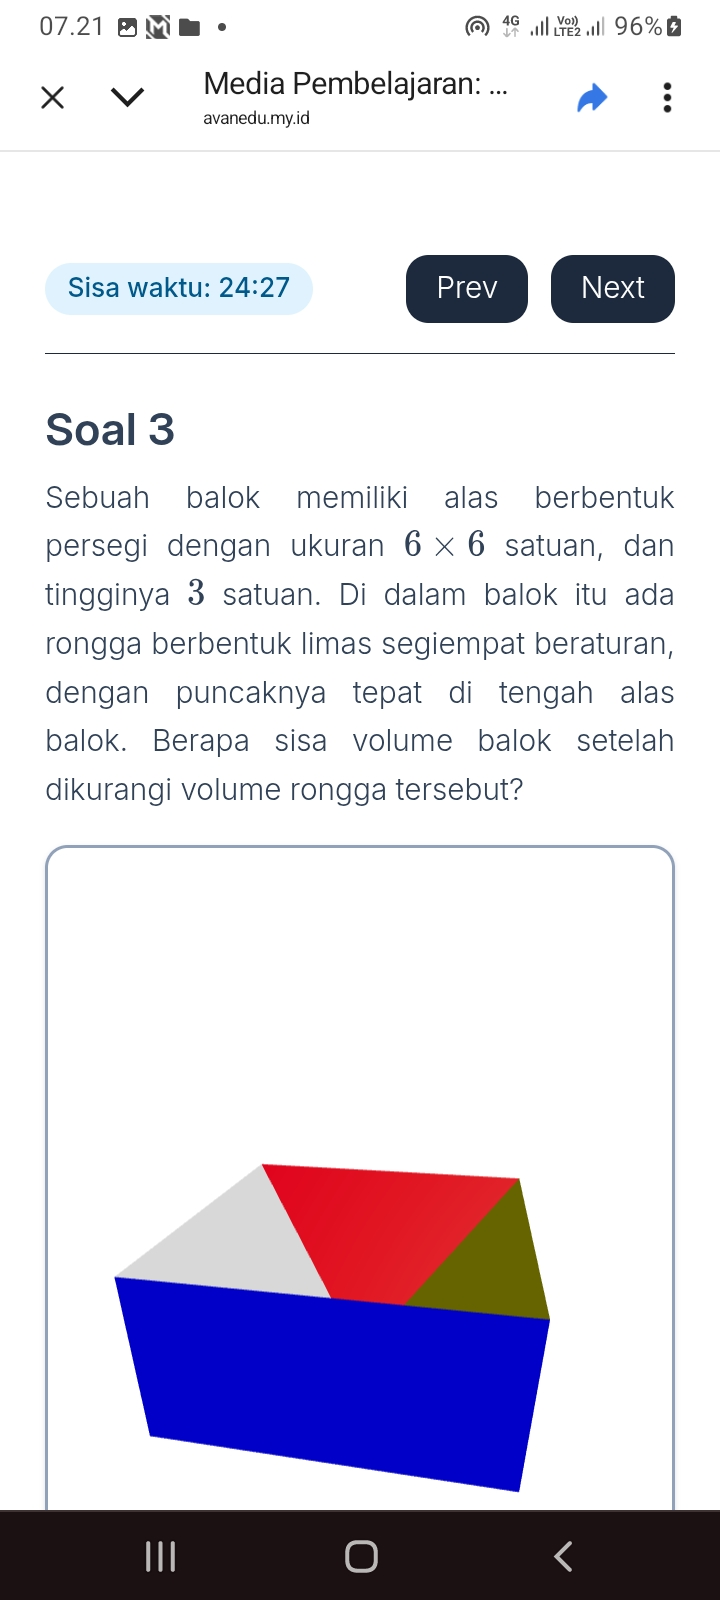
\includegraphics[width=0.25\textwidth]{images/kuis3.jpg}
        \caption{Halaman Kuis}
        \label{fig:kuis}
    \end{figure}

\end{enumerate}